% file: CompPhys.tex
% Computational Physics (notes), in unconventional ``grande'' format; fitting a widescreen format
% 
% github        : ernestyalumni
% gmail         : ernestyalumni 
% linkedin      : ernestyalumni 
% wordpress.com : ernestyalumni
%
% This code is open-source, governed by the Creative Common license.  Use of this code is governed by the Caltech Honor Code: ``No member of the Caltech community shall take unfair advantage of any other member of the Caltech community.'' 

\documentclass[10pt]{amsart}
\pdfoutput=1
%\usepackage{mathtools,amssymb,lipsum,caption}
\usepackage{mathtools,amssymb,caption}


\usepackage{graphicx}
\usepackage{hyperref}
\usepackage[utf8]{inputenc}
\usepackage{listings}
\usepackage[table]{xcolor}
\usepackage{pdfpages}
\usepackage{tikz}
\usetikzlibrary{matrix,arrows}

\usepackage{multicol}

\hypersetup{colorlinks=true,citecolor=[rgb]{0,0.4,0}}

\oddsidemargin=15pt
\evensidemargin=5pt
\hoffset-45pt
\voffset-55pt
\topmargin=-4pt
\headsep=5pt
\textwidth=1120pt
\textheight=595pt
\paperwidth=1200pt
\paperheight=700pt
\footskip=40pt








\newtheorem{theorem}{Theorem}
\newtheorem{corollary}{Corollary}
%\newtheorem*{main}{Main Theorem}
\newtheorem{lemma}{Lemma}
\newtheorem{proposition}{Proposition}

\newtheorem{definition}{Definition}
\newtheorem{remark}{Remark}

\newenvironment{claim}[1]{\par\noindent\underline{Claim:}\space#1}{}
\newenvironment{claimproof}[1]{\par\noindent\underline{Proof:}\space#1}{\hfill $\blacksquare$}

%This defines a new command \questionhead which takes one argument and
%prints out Question #. with some space.
\newcommand{\questionhead}[1]
  {\bigskip\bigskip
   \noindent{\small\bf Question #1.}
   \bigskip}

\newcommand{\problemhead}[1]
  {
   \noindent{\small\bf Problem #1.}
   }

\newcommand{\exercisehead}[1]
  { \smallskip
   \noindent{\small\bf Exercise #1.}
  }

\newcommand{\solutionhead}[1]
  {
   \noindent{\small\bf Solution #1.}
   }


\title{Computational Physics: includes Parallel Computing/Parallel Programming}
\author{Ernest Yeung \href{mailto:ernestyalumni@gmail.com}{ernestyalumni@gmail.com}}
\date{23 mai 2016}
\keywords{Computational Physics, Parallel Computing, Parallel Programming}
\begin{document}

\definecolor{darkgreen}{rgb}{0,0.4,0}
\lstset{language=C++,
  keywordstyle=\color{blue},
  stringstyle=\color{red},
 commentstyle=\color{darkgreen}
 }
%\lstlistoflistings

\maketitle

\tableofcontents


\begin{multicols*}{2}

\begin{abstract}
Everything about Computational Physics, including Parallel computing/ Parallel programming.  
\end{abstract}

\part{Introduction}

\section{Parallel Computing}

\subsection{Udacity Intro to Parallel Programming : Lesson 1 - The GPU Programming Model}

Owens and Luebki pound fists at the end of this video.  $=))))$  \href{https://classroom.udacity.com/courses/cs344/lessons/55120467/concepts/658304810923}{Intro to the class}.

\subsubsection{Running CUDA locally}
Also, \href{https://classroom.udacity.com/courses/cs344/lessons/55120467/concepts/658304810923}{Intro to the class}, in Lesson 1 - The GPU Programming Model, has links to documentation for running CUDA locally; in particular, for Linux: \url{http://docs.nvidia.com/cuda/cuda-getting-started-guide-for-linux/index.html}.  That guide told me to go download the NVIDIA CUDA Toolkit, which is the \href{NVIDIA CUDA Developer Toolkit}{https://developer.nvidia.com/cuda-downloads}.  

For \emph{Fedora}, I chose Installer Type \verb|runfile (local)|.  

Afterwards, installation of CUDA on Fedora 23 workstation had been nontrivial.  Go see either my github repository \href{https://github.com/ernestyalumni/MLgrabbag/blob/master/README.md}{MLgrabbag} (which will be updated) or my \href{https://ernestyalumni.wordpress.com/2016/05/07/fedora-23-workstation-linuxnvidia-geforce-gtx-980-ti-my-experience-log-of-what-i-do-and-find-out/#CUDAinstall}{wordpress blog} (which may not be upgraded frequently).  


$P=VI = I^2R$ heating.

\subsubsection{Definitions of Latency and throughput (or bandwidth)}

cf. 
\href{https://classroom.udacity.com/courses/cs344/lessons/55120467/concepts/669874580923}{Building a Power Efficient Processor}

\href{https://classroom.udacity.com/courses/cs344/lessons/55120467/concepts/667559300923}{Latency vs Bandwidth}

latency $[\text{sec}]$.  From the title ``Latency vs. bandwidth'', I'm thinking that throughput $=$ bandwidth (???).  throughput $ = $ job$/$time (of job).  

Given total task, velocity $v$, \\
total task $/v = $ latency.  throughput $=$ latency$/(\text{jobs per total task})$.  


Also, in \href{https://classroom.udacity.com/courses/cs344/lessons/55120467/concepts/669874580923}{Building a Power Efficient Processor}.  Owens recommends the article David Patterson, ``Latency...''

cf. \href{https://classroom.udacity.com/courses/cs344/lessons/55120467/concepts/671181630923}{GPU from the Point of View of the Developer}

$n_{\text{core}} \equiv $ number of cores \\
$n_{\text{vecop}} \equiv$ ($n_{\text{vecop}}-$wide axial vector operations$/core$ core) \\
$n_{\text{thread}} \equiv $ threads$/$core (hyperthreading)
\[
n_{\text{core}} \cdot n_{\text{vecop}} \cdot n_{\text{thread}}  \text{ parallelism  }
\]

There were various websites that I looked up to try to find out the capabilities of my video card, but so far, I've only found these commands (and I'll print out the resulting output):
{\scriptsize
\begin{lstlisting}
$ lspci -vnn | grep VGA -A 12
03:00.0 VGA compatible controller [0300]: NVIDIA Corporation GM200 [GeForce GTX 980 Ti] [10de:17c8] (rev a1) (prog-if 00 [VGA controller])
	Subsystem: eVga.com. Corp. Device [3842:3994]
	Physical Slot: 4
	Flags: bus master, fast devsel, latency 0, IRQ 50
	Memory at fa000000 (32-bit, non-prefetchable) [size=16M]
	Memory at e0000000 (64-bit, prefetchable) [size=256M]
	Memory at f0000000 (64-bit, prefetchable) [size=32M]
	I/O ports at e000 [size=128]
	[virtual] Expansion ROM at fb000000 [disabled] [size=512K]
	Capabilities: <access denied>
	Kernel driver in use: nvidia
	Kernel modules: nouveau, nvidia

$ lspci | grep VGA -E
03:00.0 VGA compatible controller: NVIDIA Corporation GM200 [GeForce GTX 980 Ti] (rev a1)

$ grep driver /var/log/Xorg.0.log
[    18.074] Kernel command line: BOOT_IMAGE=/vmlinuz-4.2.3-300.fc23.x86_64 root=/dev/mapper/fedora-root ro rd.lvm.lv=fedora/root rd.lvm.lv=fedora/swap rhgb quiet LANG=en_US.UTF-8 nouveau.modeset=0 rd.driver.blacklist=nouveau nomodeset gfxpayload=vga=normal
[    18.087] (WW) Hotplugging is on, devices using drivers 'kbd', 'mouse' or 'vmmouse' will be disabled.
[    18.087] 	X.Org XInput driver : 22.1
[    18.192] (II) Loading /usr/lib64/xorg/modules/drivers/nvidia_drv.so
[    19.088] (II) NVIDIA(GPU-0): Found DRM driver nvidia-drm (20150116)
[    19.102] (II) NVIDIA(0):     ACPI event daemon is available, the NVIDIA X driver will
[    19.174] (II) NVIDIA(0): [DRI2]   VDPAU driver: nvidia
[    19.284] 	ABI class: X.Org XInput driver, version 22.1
...

$ lspci -k | grep -A 8 VGA
03:00.0 VGA compatible controller: NVIDIA Corporation GM200 [GeForce GTX 980 Ti] (rev a1)
	Subsystem: eVga.com. Corp. Device 3994
	Kernel driver in use: nvidia
	Kernel modules: nouveau, nvidia
03:00.1 Audio device: NVIDIA Corporation GM200 High Definition Audio (rev a1)
	Subsystem: eVga.com. Corp. Device 3994
	Kernel driver in use: snd_hda_intel
	Kernel modules: snd_hda_intel
05:00.0 USB controller: VIA Technologies, Inc. VL805 USB 3.0 Host Controller (rev 01)
  \end{lstlisting}
}
\href{https://classroom.udacity.com/courses/cs344/lessons/55120467/concepts/671181640923}{CUDA Program Diagram}

\[
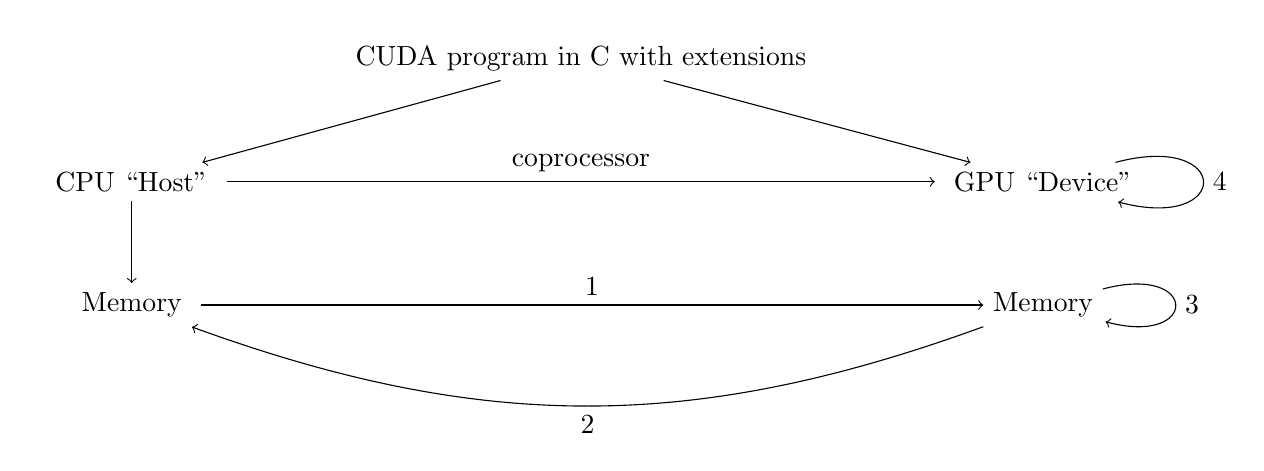
\begin{tikzpicture}
  \matrix (m) [matrix of math nodes, row sep=3em, column sep=4em, minimum width=1em]
  {
    & \text{ CUDA program in C with extensions } &  \\
    \text{ CPU ``Host'' } & & \text{ GPU ``Device'' } \\
    \text{ Memory } & & \text{Memory} \\
};
  \path[->]
  (m-1-2) edge node [above] {} (m-2-1)
  edge node [above] {} (m-2-3)
  (m-2-1) edge node [above] { coprocessor } (m-2-3)
  edge node [above] {} (m-3-1)
  (m-3-1) edge node [above] {$1$} (m-3-3)
  (m-3-3) edge [bend left=20] node [below] {$2$} (m-3-1)
  edge [loop right] node [right] {$3$} (m-3-3)
  (m-2-3) edge [loop right] node [right] {$4$} (m-2-3)
  ;
\end{tikzpicture}
\]
CPU ``host'' is the boss (and issues commands) -Owen.

$\text{Coprocessor} : \text{ CPU ``host'' } \to \text{ GPU ``device'' } $ \\
$\text{Coprocessor} : \text{ CPU process } \mapsto \text{ (co)-process out to GPU } $ \\

With
\begin{enumerate}
  \item[1] data cpu $\to $ gpu
  \item[2] data gpu $\to$ cpu \qquad (initiated by cpu host) \\

$1.,2.,$ uses \verb|cudaMemcpy| 
  \item[3] allocate GPU memory: \verb|cudaMalloc|
  \item[4] launch kernel on GPU
  \end{enumerate}
Remember that for 4., this launching of the kernel, while it's acting on GPU ``device'' onto itself, it's initiated by the boss, the CPU ``host''.

Hence, cf. \href{https://classroom.udacity.com/courses/cs344/lessons/55120467/concepts/670489380923}{Quiz: What Can GPU Do in CUDA}, GPUs can respond to CPU request to receive and send Data CPU $\to $ GPU and Data GPU $\to $ CPU, respectively (1,2, respectively), and compute a kernel launched by the CPU (3).


\href{https://classroom.udacity.com/courses/cs344/lessons/55120467/concepts/670742800923}{A CUDA Program}
A typical GPU program

\begin{itemize}
\item \verb|cudaMalloc| - CPU allocates storage on GPU 
\item \verb|cudaMemcpy| - CPU copies input data from CPU $\to $ GPU 
\item \emph{kernel launch} - CPU launches kernel(s) on GPU to process the data 
\item \verb|cudaMemcpy| - CPU copies results back to CPU from GPU
  \end{itemize}

Owens advises minimizing ``communication'' as much as possible (e.g. the \verb|cudaMemcpy| between CPU and GPU), and do a lot of computation in the CPU and GPU, each separately.

\href{https://classroom.udacity.com/courses/cs344/lessons/55120467/concepts/672300540923}{Defining the GPU Computation}

Owens circled this
{\Large
  \[
  \begin{gathered}
\text{ BIG IDEA } \qquad \, \boxed{ \text{ This is Important } }  \\
\begin{aligned} 
& \text{ Kernels look like serial programs } \\
  & \text{ Write your program as if it will run on \textbf{ one } thread } \\
  & \text{The GPU will run that program on \textbf{ many } threads}
  \end{aligned}
\end{gathered}
\]
}

\href{https://classroom.udacity.com/courses/cs344/lessons/55120467/concepts/670742840923}{Squaring A Number on the CPU}

Note
\begin{enumerate}
\item Only 1 thread of execution: (``thread'' $:=$ one independent path of execution through the code) e.g. the \verb|for| loop
  \item no explicit parallelism; it's serial code e.g. the \verb|for| loop through 64 elements in an array
  \end{enumerate}


\href{https://classroom.udacity.com/courses/cs344/lessons/55120467/concepts/670742870923}{GPU Code A High Level View}

CPU:
\begin{itemize}
  \item Allocate Memory 
  \item Copy Data to/from GPU
    \item Launch Kernel - species degree of parallelism
\end{itemize}

GPU:
\begin{itemize}
\item Express Out $=$ In $\cdot $ In  - says \emph{nothing} about the degree of parallelism
  \end{itemize}

Owens reiterates that in the GPU, everything looks serial, but it's only in the CPU that anything parallel is specified.  

pseudocode: CPU code: square kernel $<<< 64 >>>$ (outArray,inArray)

\href{https://classroom.udacity.com/courses/cs344/lessons/55120467/concepts/670742940923}{Squaring Numbers Using CUDA Part 3}

From the example
\begin{lstlisting}
  // launch the kernel
  square<<<1, ARRAY_SIZE>>>(d_out, d_in)
  \end{lstlisting}
we're introduced to the ``CUDA launch operator'', initiating a kernel of 1 block of 64 elements (\verb|ARRAY_SIZE| is 64) on the GPU.  Remember that \verb|d_| prefix (this is naming comvention) tells us it's on the device, the GPU, solely.  

With CUDA launch operator $\equiv <<<>>>$, then also looking at this explanation on \verb|stackexchange| (so surely others are confused as well, of those who are learning this (cf. \href{http://stackoverflow.com/questions/19240658/cuda-kernel-launch-parameters-explained-right}{CUDA kernel launch parameters explained right?}).  From \href{http://stackoverflow.com/users/1957265/eric}{Eric}'s answer, \\

threads are grouped into blocks.  all the threads will execute the invoked kernel function.

Certainly,
\[
\begin{aligned}
  & <<<>>>:(n_{\text{block}}, n_{\text{threads}})\times \text{kernelfunctions} \mapsto \text{kernelfunction}<<<n_{\text{block}},n_{\text{threads}}>>> \in \text{End}:\text{Dat}_{\text{GPU}} \\ 
  & <<<>>>: \mathbb{N}^+ \times \mathbb{N}^+ \times \text{Mor}_{\text{GPU}} \to \text{End}\text{Dat}_{\text{GPU}}
  \end{aligned}
\]
where I propose that GPU can be modeled as a category containing objects $\text{Dat}_{\text{GPU}}$, the collection of all possible data inputs and outputs into the GPU, and $\text{Mor}_{\text{GPU}}$, the collection of all kernel functions that run (exclusively, and this \emph{must} be the class, as reiterated by Prof. Owen) on the GPU.

Next,
\[
\begin{aligned}
  & \text{kernelfunction}<<<n_{\text{block}},n_{\text{threads}}>>>: \text{din}\mapsto \text{dout} \qquad \, (\text{as given in the ``square'' example, and so I propose}) \\ 
  & \text{kernelfunction}<<<n_{\text{block}},n_{\text{threads}}>>>:(\mathbb{N}^+)^{n_{\text{threads}}} \to (\mathbb{N}^+)^{n_{\text{threads}}}
  \end{aligned}
\]
But keep in mind that $\text{dout}$, $\text{din}$ are pointers in the C program, pointers to the place in the memory.  

\verb|cudaMemcopy| is a functor category, s.t. e.g. $\text{Obj}_{\text{CudaMemcopy}} \ni \text{cudaMemcpyDevicetoHost}$ where
\[
\text{cudaMemcopy}(-,-,n_{\text{thread}},\text{cudaMemcpyDeviceToHost}): \text{Memory}_{\text{GPU}} \to \text{Memory}_{\text{CPU}} \in \text{Hom}(\text{Memory}_{\text{GPU}}, \text{Memory}_{\text{CPU}})
\]

\href{https://classroom.udacity.com/courses/cs344/lessons/55120467/concepts/670742910923}{Squaring Numbers Using CUDA 4}

Note the C language construct \emph{declaration specifier} - denotes that this is a kernel (for the GPU) and not CPU code.  Pointers need to be allocated on the GPU (otherwise your program will crash spectacularly -Prof. Owen).  

\subsubsection{What are C pointers?}

Is $\langle \text{ type } \rangle \, *$, a pointer, then a mapping from the category, namely the objects of types, to a mapping from the specified value type to a memory address?

e.g.
\[
\begin{aligned}
  \langle \, \rangle \, * & : \text{float} \mapsto \text{float} \, * \\ 
  \text{float } \, * & : \text{din} \mapsto \text{ some memory address }
\end{aligned}
\]
and then we pass in mappings, not values, and so we're actually declaring a square \emph{functor}.

What is \verb|threadIdx|?  What is it mathematically?  Consider that $\exists \,$ 3 ``modules'':

\[
\begin{aligned}
  & \text{threadIdx}.x \\
  & \text{threadIdx}.y \\
  & \text{threadIdx}.z 
\end{aligned}
\]
And then the line
\begin{lstlisting}
int idx = threadIdx.x;
  \end{lstlisting}
says that idx is an integer, ``declares'' it to be so, and then assigns idx to $\text{threadIdx}.x$ which surely has to also have the same type, integer.  So (perhaps)
\[
idx \equiv \text{threadIdx}.x \in \mathbb{Z}
\]
is the same thing.

Then suppose threadIdx $\subset \mathbf{\text{FinSet}}$, a subcategory of the category of all (possible) finite sets, s.t. threadIdx has 3 particular morphisms, $x,y,z\in \text{Mor}threadIdx$,
\[
\begin{aligned}
  & x : \text{threadIdx} \mapsto \text{threadIdx}.x \in \text{Obj}_{\mathbf{\text{FinSet}}} \\ 
  & y : \text{threadIdx} \mapsto \text{threadIdx}.x \in \text{Obj}_{\mathbf{\text{FinSet}}} \\ 
  & z : \text{threadIdx} \mapsto \text{threadIdx}.x \in \text{Obj}_{\mathbf{\text{FinSet}}}  
\end{aligned}
\]

\href{https://classroom.udacity.com/courses/cs344/lessons/55120467/concepts/670742980923}{Configuring the Kernel Launch Parameters Part 1}

$n_{\text{blocks}}$, $n_{\text{threads}}$ with $n_{\text{threads}} \geq 1024$ (this maximum constant is GPU dependent).  You should pick the $(n_{\text{blocks}}, n_{\text{threads}})$ that makes sense for your problem, says Prof. Owen.  

\subsubsection{More thoughts on Squaring Numbers Using CPU, and then using CUDA}

Note that this squaring of numbers is really element-wise multiplication of a vector.

I sought an isomorphism between abstract algebra and computer code.

Consider
\[
\begin{aligned}
 &  \mathbb{R}^N \ni x \qquad \, N \in \mathbb{Z}^+ \\ 
 &  \mathbb{R} \ni x[i] \qquad i = 1 \dots N \to i = 0, \dots N-1 
  \end{aligned}
\]
Then the element-wise squaring of numbers is
\[
(x[i])^2 = x[i] \cdot x[i]
\]
In general,
\[
(x[i])^p = \underbrace{x[i]\cdot x[i] \dots x[i]}_{ p \text{ times } }
\]

\subsubsection{Memory layout of blocks and threads}

$\forall \, (n_{\text{blocks}}, n_{\text{threads}}) \in \mathbb{Z} \times \lbrace 1 \dots 1024 \rbrace$, $\lbrace 1 \dots n_{\text{block}} \times \lbrace 1 \dots n_{\text{threads}} \rbrace$ is now an ordered index (with lexicographical ordering).  This is just 1-dimensional (so possibly there's a 1-to-1 mapping to a finite subset of $\mathbb{Z}$).

I propose that ``adding another dimension'' or the 2-dimension, that Prof. Owen mentions is being able to do the Cartesian product, up to 3 Cartesian products, of the block-thread index.  

\href{https://classroom.udacity.com/courses/cs344/lessons/55120467/concepts/668398860923}{Quiz: Configuring the Kernel Launch Parameters 2 }

Most general syntax:

Configuring the kernel launhc
\begin{lstlisting}
  kernel<<<grid of blocks, block of threads >>>(...)

  // for example

  square<<<dim3(bx,by,bz), dim3(tx,ty,tz), shmem>>>(...)
  \end{lstlisting}
where \verb|dim3(tx,ty,tz)| is the grid of blocks $bx\cdot by \cdot bz$ \\
\phantom{ where } \verb|{dim3}(tx,ty,tz)| is the block of threads $tx \cdot ty \cdot tz$ \\
\phantom{ where } \verb|shmem| is the shared memory per block in bytes


\href{https://classroom.udacity.com/courses/cs344/lessons/55120467/concepts/673071460923#}{Quiz: Map}

I wanted to try to mathematically formulate the idea of \verb|map|.

\[
\begin{gathered}
  \verb|MAP(ELEMENTS,FUNCTION)|
  \end{gathered} \Longleftrightarrow
\begin{gathered}
\begin{gathered}
  \text{ given } x \in \mathbb{R}^N \\ 
  x[i] \xrightarrow{ f } f(x[i]) 
\end{gathered} \\
\text{ or } \\ 
\begin{gathered}
  \text{ set of elements (finite, so can be indexed) } \qquad \, \lbrace x_0 , \dots , x_{n-1} \rbrace_{\mathcal{A}} \in \text{Obj}\mathbf{ \text{Fin} } \\
  x_i \xrightarrow{ f } f(x_i) , \qquad \, \forall \, i \in \mathcal{A}
  \end{gathered}
  \end{gathered}
\]

\href{https://classroom.udacity.com/courses/cs344/lessons/55120467/concepts/967066740923}{Problem Set 1}
``Also, the image is represented as an 1D array in the kernel, not a 2D array like I mentioned in the video.''

Here's part of that code for squaring numbers:
\begin{lstlisting}
  __global__ void square(float *d_out, float *d_in) {
    int idx = threadIdx.x;
    float f = d_in[idx];
    d_out[idx] = f*f;
    }
  \end{lstlisting}

\subsubsection{Problem Set 1, Udacity CS344}

Let $\begin{aligned} & \quad \\
  & L_x \equiv \text{ total number of pixels in $x$-direction of image } \in \mathbb{Z}^+ \\
   & L_y \equiv \text{ total number of pixels in $y$-direction of image } \in \mathbb{Z}^+ \end{aligned}$

and so $L_x L_y  = $ total number of pixels in image.

The formula for ensuring that all threads will be computed, given an arbitrary choice of the number of threads in a (single) block, is the following:

\[
\begin{aligned}
  & \frac{L_x + ( M_x - 1) }{ M_x} = N_x \in \mathbb{N} \qquad \, & N_x = \text{ number of (thread) blocks in $x$-direction } \\ 
  & \frac{L_y + ( M_y - 1) }{ M_y} = N_y \in \mathbb{N} \qquad \, & N_y = \text{ number of (thread) blocks in $y$-direction } 
\end{aligned}
\]

Then
\[
(M_x, M_y, 1) \in \mathbb{N}^3  \Longleftrightarrow \verb|dim3|
\]
needs to be determined manually, empirically, and in consideration of the actual GPU hardware architecture (look up number of CUDA cores, and allowed maximum threads), where
\[
\begin{aligned}
  & M_x \equiv \text{ number of threads per block in $x$-direction } \\ 
  & M_y \equiv \text{ number of threads per block in $y$-direction } 
  \end{aligned}
\]

Consider that we want to go from the indices on each thread per block, on each block on the grid, in each of the 2 dimensions, to a global 2-dimensional position, and then ``flatten'' these coordinates to a 1-dimensional array that CUDA C can load onto global memory.  In other words, for

\[
\begin{gathered}
\begin{aligned}  
  & i_x \in \lbrace 0 , \dots , M_x - 1 \rbrace \qquad \, & \Longleftrightarrow \verb| threadIdx.x| \\ 
  & i_y \in \lbrace 0 , \dots , M_y - 1 \rbrace \qquad \, & \Longleftrightarrow \verb| threadIdx.y|
  \end{aligned} \\ 
\begin{aligned}
  & j_x \in \lbrace 0 , \dots , N_x - 1 \rbrace \qquad \, & \Longleftrightarrow \verb| blockIdx.x| \\ 
  & j_y \in \lbrace 0 , \dots , N_y - 1 \rbrace \qquad \, & \Longleftrightarrow \verb| blockIdx.y|
  \end{aligned}
\end{gathered}
\]

and so for
\[
\begin{gathered}
  (k_x,k_y) \\
\begin{aligned}
  & k_X = i_x + j_x M_x \\ 
  & k_y = i_y + j_y M_y
  \end{aligned} 
  \end{gathered}
\]

then we sought the following operations:
\[
\begin{gathered}
  (j_x,j_y)\times (i_x,i_y) \in \lbrace 0 , \dots , N_x - 1 \rbrace \times \lbrace 0 \dots N_y - 1 \rbrace \times \lbrace 0 \dots M_x - 1 \rbrace \times \lbrace 0 \dots M_y - 1 \rbrace \in \verb|dim3| \times \verb|dim3| \\
  \mapsto (k_x,k_y) \in \lbrace 0 \dots L_x -1 \rbrace \times \lbrace 0 \dots L-y - 1 \rbrace \\
  \mapsto k = k_x + L_x k_y \in \lbrace 0 \dots L_x L_y - 1 \rbrace 
  \end{gathered}
\]

\subsubsection{Grid of blocks, block of threads, thread that's indexed; (mathematical) structure of it all}

Let
\[
\begin{gathered}
  \text{grid} = \prod_{I=1}^N (\text{block})^{n_I^{\text{block}}}
\end{gathered}
\]
where $N=1,2,3$ (for CUDA) and by naming convention $\begin{aligned} & \quad \\
  & I = 1 \equiv x \\
  & I = 2 \equiv y \\
  & I = 3 \equiv z \end{aligned}$

Let's try to make it explicitly (as others had difficulty understanding the grid, block, thread model, cf. \href{http://stackoverflow.com/questions/14711668/colored-image-to-greyscale-image-using-cuda-parallel-processing}{colored image to greyscale image using CUDA parallel processing}, \href{http://stackoverflow.com/questions/16619274/cuda-griddim-and-blockdim}{Cuda gridDim and blockDim}) through commutative diagrams and categories (from math):

\[
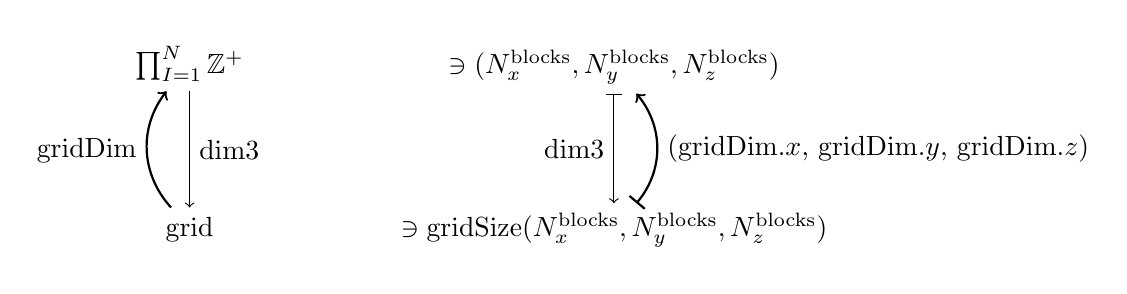
\begin{tikzpicture}
  \matrix (m) [matrix of math nodes, row sep=4em, column sep=5em, minimum width=2em]
  {
\prod_{I=1}^N \mathbb{Z}^+ & \ni (N_x^{\text{blocks}}, N_y^{\text{blocks}} , N_z^{\text{blocks}}) \\
\text{grid} & \ni \text{gridSize}(N_x^{\text{blocks}}, N_y^{\text{blocks}} , N_z^{\text{blocks}} ) \\
};
  \path[->]
  (m-1-1) edge node [right] {$\text{dim}3$} (m-2-1)
  (m-2-1) edge [bend left=40, thick] node [left] {$\text{gridDim}$} (m-1-1)
  ;
  \path[|->]
  (m-1-2) edge node [left] {$\text{dim}3$} (m-2-2)
  (m-2-2) edge [bend right=40, thick] node [right] {$(\text{gridDim}.x$, $\text{gridDim}.y$, $\text{gridDim}.z)$} (m-1-2)
  ;  
\end{tikzpicture}
\]

\[
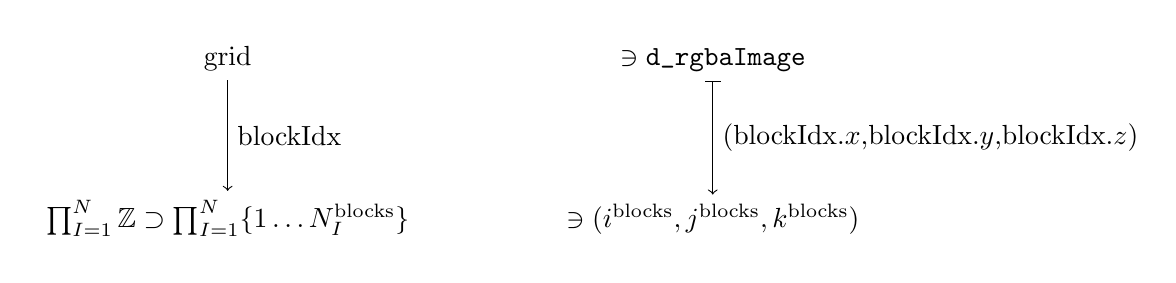
\begin{tikzpicture}
  \matrix (m) [matrix of math nodes, row sep=4em, column sep=5em, minimum width=2em]
  {
    \text{grid} & \ni \verb|d_rgbaImage| \\
    \prod_{I=1}^N \mathbb{Z} \supset \prod_{I=1}^N \lbrace 1 \dots N_I^{\text{blocks}} \rbrace & \ni (i^{\text{blocks}},j^{\text{blocks}}, k^{\text{blocks}} ) \\
};
  \path[->]
  (m-1-1) edge node [right] {$\text{blockIdx}$} (m-2-1)
  ;
  \path[|->]
  (m-1-2) edge node [right] {($\text{blockIdx}.x$,$\text{blockIdx}.y$,$\text{blockIdx}.z$)} (m-2-2)
  ;
  \end{tikzpicture}
\]

and then similar relations (i.e. arrows, i.e. relations) go for a block of threads:

\[
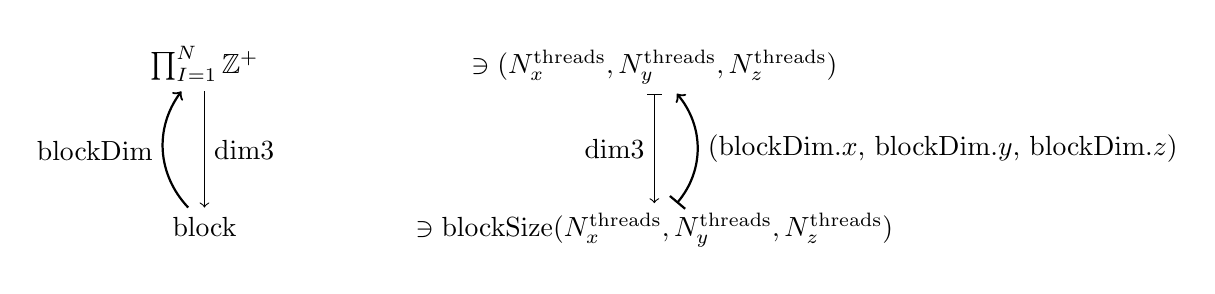
\begin{tikzpicture}
  \matrix (m) [matrix of math nodes, row sep=4em, column sep=5em, minimum width=2em]
  {
\prod_{I=1}^N \mathbb{Z}^+ & \ni (N_x^{\text{threads}}, N_y^{\text{threads}} , N_z^{\text{threads}}) \\
\text{block} & \ni \text{blockSize}(N_x^{\text{threads}}, N_y^{\text{threads}} , N_z^{\text{threads}} ) \\
};
  \path[->]
  (m-1-1) edge node [right] {$\text{dim}3$} (m-2-1)
  (m-2-1) edge [bend left=40, thick] node [left] {$\text{blockDim}$} (m-1-1)
  ;
  \path[|->]
  (m-1-2) edge node [left] {$\text{dim}3$} (m-2-2)
  (m-2-2) edge [bend right=40, thick] node [right] {$(\text{blockDim}.x$, $\text{blockDim}.y$, $\text{blockDim}.z)$} (m-1-2)
  ;  
\end{tikzpicture}
\]

\[
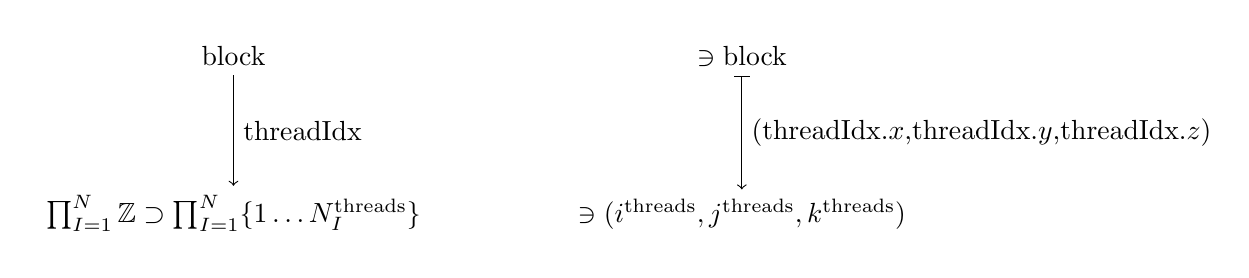
\begin{tikzpicture}
  \matrix (m) [matrix of math nodes, row sep=4em, column sep=5em, minimum width=2em]
  {
    \mathbf{\text{block}} & \ni \text{block} \\
    \prod_{I=1}^N \mathbb{Z} \supset \prod_{I=1}^N \lbrace 1 \dots N_I^{\text{threads}} \rbrace & \ni (i^{\text{threads}},j^{\text{threads}}, k^{\text{threads}} ) \\
};
  \path[->]
  (m-1-1) edge node [right] {$\text{threadIdx}$} (m-2-1)
  ;
  \path[|->]
  (m-1-2) edge node [right] {($\text{threadIdx}.x$,$\text{threadIdx}.y$,$\text{threadIdx}.z$)} (m-2-2)
  ;
  \end{tikzpicture}
\]

\href{https://discussions.udacity.com/t/gridsize-help-assignment-1-pp/124701}{gridsize help assignment 1 Pp} explains how threads per block is variable, and remember how Owens said Luebki says that a GPU doesn't get up for more than a 1000 threads per block.  

\subsubsection{Generalizing the model of an image}

Consider vector space $V$, e.g. $\text{dim}V=4$, vector space $V$ over field $\mathbb{K}$, so $V= \mathbb{K}^{\text{dim}V}$.

Each pixel represented by $\forall \, v \in V$.

Consider an image, or space, $M$.  $\text{dim}M = 2$ (image), $\text{dim}M=3$.  Consider a local chart (that happens to be global in our case):
\[
\begin{aligned}
  & \varphi : M \to \mathbb{Z}^{\text{dim}M} \supset \lbrace 1 \dots N_1 \rbrace \times \lbrace 1 \dots N_2 \rbrace \times \dots \times \lbrace 1 \dots N_{\text{dim}M} \rbrace \\ 
  & \varphi : x \mapsto (x^1(x), x^2(x), \dots , x^{\text{dim}M}(x) )
  \end{aligned}
\]
\[
\begin{tikzpicture}
  \matrix (m) [matrix of math nodes, row sep=4em, column sep=5em, minimum width=2em]
  {
    E & M \times V \\ 
    M &  \\
};
  \path[->]
  (m-1-1) edge node [auto] {$\varphi$} (m-1-2)
          edge node [left] {$\pi$} (m-2-1)
  (m-1-2) edge node [auto] {$$} (m-2-1)
              ;
  \end{tikzpicture}
\qquad \, 
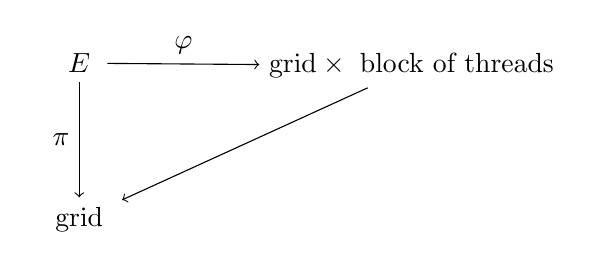
\begin{tikzpicture}
  \matrix (m) [matrix of math nodes, row sep=4em, column sep=5em, minimum width=2em]
  {
    E & \text{grid} \times \text{ block of threads } \\ 
    \text{ grid } & \\
};
  \path[->]
  (m-1-1) edge node [auto] {$\varphi$} (m-1-2)
          edge node [left] {$\pi$} (m-2-1)
  (m-1-2) edge node [auto] {$$} (m-2-1)
              ;
  \end{tikzpicture}
\]

Consider a ``coarsing'' of underlying $M$:
\[
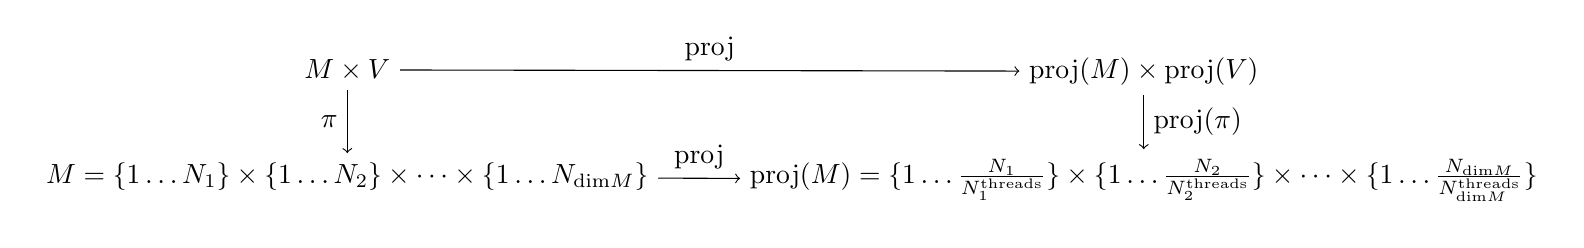
\begin{tikzpicture}
  \matrix (m) [matrix of math nodes, row sep=2em, column sep=3em, minimum width=1em]
  {
    M\times V & \text{proj}(M) \times \text{proj}(V) \\ 
    M = \lbrace 1 \dots N_1 \rbrace \times \lbrace 1 \dots N_2 \rbrace \times \dots \times \lbrace 1 \dots N_{\text{dim}M} \rbrace  & \text{proj}(M)  = \lbrace 1 \dots \frac{N_1}{N_1^{\text{threads}} } \rbrace \times \lbrace 1 \dots \frac{N_2}{N_2^{\text{threads}} } \rbrace \times \dots \times \lbrace 1 \dots \frac{N_{\text{dim}M}}{N_{\text{dim}M}^{\text{threads}} } \rbrace \\  
};
  \path[->]
  (m-1-1) edge node [auto] {$\text{proj}$} (m-1-2)
          edge node [left] {$\pi$} (m-2-1)
  (m-1-2) edge node [auto] {$\text{proj}(\pi)$} (m-2-2)
  (m-2-1) edge node [auto] {$\text{proj}$} (m-2-2)        
          ;
  \end{tikzpicture}
\]
e.g. $\begin{aligned} & \quad \\
  & N_1^{\text{thread}} = 12 \\
  & N_2^{\text{thread}} = 12 \end{aligned}$

Just note that in terms of syntax, you have the ``block'' model, in which you allocate blocks along each dimension.  So in
\[
\begin{aligned}
  & const \; dim3 \; blockSize(n^b_x, n^b_y, n^b_z) \\
  & const \; dim3 \; gridSize(n^{\text{gr}}_x, n^{\text{gr}}_y, n^{\text{gr}}_z)
  \end{aligned}
\]
Then the condition is
$n_x^b/\text{dim}V , n_y^b/\text{dim}V, n_z^b/\text{dim}V \in \mathbb{Z}$ (condition), \qquad \, $(n_x^{\text{gr}}-1)/\text{dim}V , n_y^{\text{gr}}/\text{dim}V, n_z^{\text{gr}}/\text{dim}V \in \mathbb{Z}$

\subsection{Unit 2, Lesson 2 GPU Hardware and Parallel Communication Patterns}

\href{https://classroom.udacity.com/courses/cs344/lessons/77202674/concepts/773931440923}{Transpose Part 1}

Now
\[
\begin{gathered}
  \begin{aligned}
    & \text{Mat}_{\mathbb{F}}(n,n) \xrightarrow{T} \text{Mat}_{\mathbb{F}}(n,n) \\ 
    & A\mapsto A^T \text{ s.t. } (A^T)_{ij} = A_{ji}
    \end{aligned} \\ 
\begin{aligned}
  &  \text{Mat}_{\mathbb{F}} \xrightarrow{T} \mathbb{F}^{n^2} \\
  & A_{ij} \mapsto A_{ij} = A_{in + j }
  \end{aligned}
\end{gathered}
\]
\[
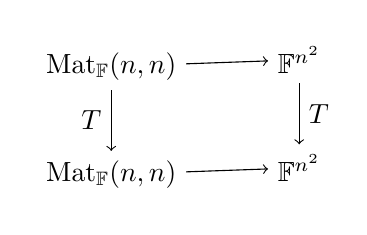
\begin{tikzpicture}
  \matrix (m) [matrix of math nodes, row sep=2em, column sep=3em, minimum width=1em]
  {
    \text{Mat}_{\mathbb{F}}(n,n) & \mathbb{F}^{n^2} \\
    \text{Mat}_{\mathbb{F}}(n,n) & \mathbb{F}^{n^2} \\ 
  };
  \path[->]
  (m-1-1) edge node [auto] {$$} (m-1-2)
          edge node [left] {$T$} (m-2-1)
  (m-1-2) edge node [auto] {$T$} (m-2-2)
  (m-2-1) edge node [auto] {$$} (m-2-2)        
          ;
  \end{tikzpicture} \qquad \, 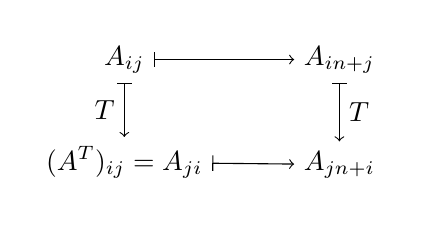
\begin{tikzpicture}
  \matrix (m) [matrix of math nodes, row sep=2em, column sep=3em, minimum width=1em]
  {
A_{ij} & A_{in+j} \\ 
(A^T)_{ij} = A_{ji} & A_{jn+i} \\
  };
  \path[|->]
  (m-1-1) edge node [auto] {$$} (m-1-2)
          edge node [left] {$T$} (m-2-1)
  (m-1-2) edge node [auto] {$T$} (m-2-2)
  (m-2-1) edge node [auto] {$$} (m-2-2)        
          ;
  \end{tikzpicture}
\]

\href{https://classroom.udacity.com/courses/cs344/lessons/77202674/concepts/773153710923}{Transpose Part 2}

Possibly, transpose is a functor.

Consider struct as a category.  In this special case, $\text{Obj}\text{struct} = \lbrace \text{arrays} \rbrace$ (a struct of arrays).  Now this struct already has a hash table for indexing upon declaration (i.e. ``creation''): so this category struct will need to be equipped with a ``diagram'' from the category of indices $J$ to struct: $J\to $ struct.

So possibly
\[
\begin{aligned}
  \text{struct} & \xrightarrow{T} & \text{ array } \\ 
 \text{Obj}\text{Struct} = \lbrace \text{ arrays } \rbrace & \xrightarrow{T} & \text{Obj}\text{array} = \lbrace \text{ struct } \rbrace \\ 
 J\to \text{ struct } & \xrightarrow{T} & J \to \text{ array } 
  \end{aligned}
\]







\href{https://classroom.udacity.com/courses/cs344/lessons/77202674/concepts/787012800923}{Quiz: What Kind Of Communication Pattern}
This quiz made a few points that clarified the characteristics of these so-called communication patterns (amongst the memory?)

\begin{itemize}
  \item map is bijective, and map $:\text{Idx} \to \text{Idx}$
  \item gather - not necessarily surjective
  \item scatter - not necessarily surjective 
  \item stencil - surjective
  \item transpose (see before)
  \end{itemize}




\href{https://classroom.udacity.com/courses/cs344/lessons/77202674/concepts/773153720923}{Parallel Communication Patterns Recap}

\begin{itemize}
\item map - bijective
\item transpose - bijective
\item gather - not necessarily surjective, and is many-to-one (by def.)
\item scatter - one-to-many (by def.) and is not necessarily surjective
\item stencil - several-to-one (not injective, by definition), and is surjective
\item reduce - all-to-one
  \item scan/sort - all-to-all
\end{itemize}

\href{https://classroom.udacity.com/courses/cs344/lessons/77202674/concepts/773153760923}{Programmer View of the GPU}

thread blocks: group of threads that cooperate to solve a (sub)problem

\href{https://classroom.udacity.com/courses/cs344/lessons/77202674/concepts/773153770923}{Thread Blocks And GPU Hardware}

CUDA GPU is a bunch of SMs:

Streaming Multiprocessors (SM)s

SMs have a bunch of simple processors and memory.

Dr. Luebki:
\[
\boxed{ \begin{gathered}
    \text{Let me say that again because it's really important} \\
    \text{GPU is responsible for allocating blocks to SMs}
  \end{gathered}
  }
\]
Programmer only gives GPU a pile of blocks.

\href{https://classroom.udacity.com/courses/cs344/lessons/77202674/concepts/787721730923}{Quiz: What Can The Programmer Specify}

I myself thought this was a revelation and was not intuitive at first:

Given a single kernel that's launched on many thread blocks include $X$, $Y$, the programmer cannot specify the sequence the blocks, e.g. block $X$, block $Y$, run (same time, or run one after the other), and which SM the block will run on (GPU does all this).  

\href{https://classroom.udacity.com/courses/cs344/lessons/77202674/concepts/787981160923}{Quiz: A Thread Block Programming Example}

Open up \verb|hello blockIdx.cu| in Lesson 2 Code Snippets (I got the repository from github, repo name is cs344).

At first, I thought you can do a single file compile and run in Eclipse without creating a new project.  No.  cf. \href{http://stackoverflow.com/questions/17164197/eclipse-creating-projects-every-time-to-run-a-single-file}{Eclipse creating projects every time to run a single file?}.  

%I opened it up in Eclipse with File, Open File (no need to create a new project).

I ended up creating a new CUDA C/C$++$ project from File -> New project, and then chose project type Executable, Empty Project, making sure to include Toolchain CUDA Toolkit (my version is 7.5), and chose an arbitrary project name (I chose cs344single).  Then, as suggested by \href{http://stackoverflow.com/users/3720356/kenny-nguyen}{Kenny Nguyen}, I dragged and dropped files into the folder, from my file directory program.

I ran the program with the ``Play'' triangle button, clicking on the green triangle button, and it ran as expected.  I also turned off Build Automatically by deselecting the option (no checkmark).

\href{https://classroom.udacity.com/courses/cs344/lessons/77202674/concepts/773883100923}{GPU Memory Model}

\[
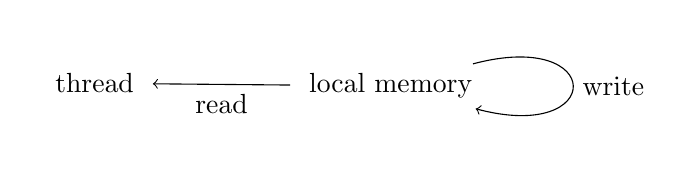
\begin{tikzpicture}
  \matrix (m) [matrix of math nodes, row sep=4em, column sep=5em, minimum width=2em]
  {
\text{ thread } & \text{ local memory } \\
};
  \path[->]
  (m-1-2) edge node [auto] {$\text{read}$} (m-1-1)
  (m-1-2) edge [loop right] node [right] {$\text{write}$} (m-1-2)
  ;
  \end{tikzpicture}
\]

Then consider threadblock $\equiv$  thread block \\
\phantom{Then consider } $\text{Obj}\text{threadblock} \supset \lbrace \text{ threads } \rbrace$ \\
\phantom{Then consider } $\text{FinSet} \xrightarrow{ \text{ threadIdx} } \text{ thread } \in \text{Mor}\text{threadblock}$

\[
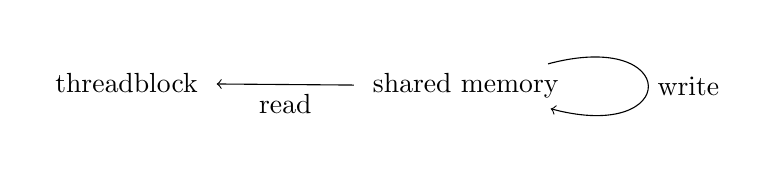
\begin{tikzpicture}
  \matrix (m) [matrix of math nodes, row sep=4em, column sep=5em, minimum width=2em]
  {
\text{ threadblock } & \text{ shared memory } \\
};
  \path[->]
  (m-1-2) edge node [auto] {$\text{read}$} (m-1-1)
  (m-1-2) edge [loop right] node [right] {$\text{write}$} (m-1-2)
  ;
  \end{tikzpicture}
\]
$\forall \, $ thread,
\[
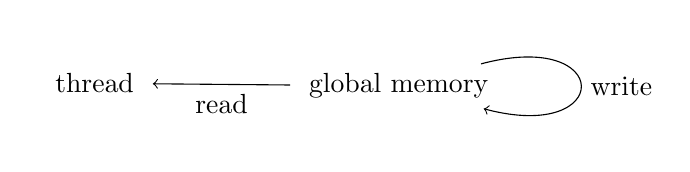
\begin{tikzpicture}
  \matrix (m) [matrix of math nodes, row sep=4em, column sep=5em, minimum width=2em]
  {
\text{ thread } & \text{ global memory } \\
};
  \path[->]
  (m-1-2) edge node [auto] {$\text{read}$} (m-1-1)
  (m-1-2) edge [loop right] node [right] {$\text{write}$} (m-1-2)
  ;
  \end{tikzpicture}
\]

\href{https://classroom.udacity.com/courses/cs344/lessons/77202674/concepts/773883130923}{Synchronization - Barrier}

Danger: what if a thread reads a result before another thread writes it?

Threads need to \emph{synchronize}.

one of the most fundamental problems in parallel computing

\href{https://classroom.udacity.com/courses/cs344/lessons/77202674/concepts/785776150923}{Quiz: The Need For Barriers}

3 barriers were needed (wasn't obvious to me at first).  All threads need to finish the write, or initialization, so it'll need a barrier.

While
\begin{lstlisting}
array[idx] = array[idx+1];
  \end{lstlisting}
is 1 line, it'll actually need 2 barriers; first read.  Then write.

So \emph{actually} we'll need to \emph{rewrite} this code:
\begin{lstlisting}
  int temp = array[idx+1];
  __syncthreads();
  array[idx] = temp;
  __syncthreads();
  \end{lstlisting}

Make sure each \emph{read} and \emph{write} operation is completed.  

kernels have implicit barrier for each.  

\href{https://classroom.udacity.com/courses/cs344/lessons/77202674/concepts/774332060923}{Writing Efficient Programs}

\begin{enumerate}
\item Maximize \emph{arithmetic intensity}
  arithmetic intensity $:= \frac{ \text{ math } }{ \text{ memory }}$
  \end{enumerate}

\href{https://classroom.udacity.com/courses/cs344/lessons/77202674/concepts/774332070923}{video: Minimize Time Spent On Memory}

local memory is fastest; global memory is slower

\[
\text{local} > \text{ shared} >> \text{global} >> \text{CPU}
\]

kernel we know (in the code) is tagged with \verb|__global__|




\subsubsection{Coalesce global memory accesses}

\href{https://classroom.udacity.com/courses/cs344/lessons/77202674/concepts/799933660923}{Coalesce Memory Access}

We saw such access pattern is coalesced; GPU must efficient when threads read or write contiguous memory locations.  


\href{https://classroom.udacity.com/courses/cs344/lessons/77202674/concepts/814086830923}{quiz: A Quiz on Coalescing Memory Access}

Work it out as Dr. Luebki did to figure out if it's coalesced memory access or not.  


\href{https://classroom.udacity.com/courses/cs344/lessons/77202674/concepts/774332150923}{Atomic Memory Operations}

Atomic Memory Operations

atomicadd atomicmin atomicXOR atomicCAS Compare And Swap


\subsubsection{On Problem Set 2}

There is what I call the ``naive global memory'' scheme, that solves the objective of blurring a photo with a local stencil of the values, using only global memory on the GPU.

Given image of size $L_x \times L_y$, i.e. $(L_x,L_y) \in (\mathbb{Z}^+)^2$; image is really a designated or particular mapping $f$,
\[
\begin{aligned}
  & f: \lbrace 0 \dots L_x - 1 \rbrace \times \lbrace 0 \dots L_y - 1 \rbrace \to \lbrace 0 \dots 255 \rbrace^4 \\ 
  & f(x,y) = (f^{(r)}(x,y) , f^{(b)}(x,y), f^{(g)}(x,y), f^{(\alpha)}(x,y) )
\end{aligned}
\]
Consider ``naive global memory scheme'' - establishing the following notation:
\[
\begin{gathered}
  \begin{aligned}
    & i_x \in \lbrace 0 \dots M_x - 1 \rbrace \Longleftrightarrow \verb|threadIdx.x| \\
    & i_y \in \lbrace 0 \dots M_y - 1 \rbrace \Longleftrightarrow \verb|threadIdx.y|  \\
    & j_x \in \lbrace 0 \dots N_x - 1 \rbrace \Longleftrightarrow \verb|blockIdx.x|  \\
    & j_y \in \lbrace 0 \dots N_y - 1 \rbrace \Longleftrightarrow \verb|blockIdx.y|  
  \end{aligned} \\
  \begin{aligned}
    & M_x \in \lbrace 1 \dots 1024 \rbrace \Longleftrightarrow \verb|blockDim.x| \\ 
    & M_y \in \lbrace 1 \dots 1024 \rbrace \Longleftrightarrow \verb|blockDim.y| 
    \end{aligned}
\end{gathered}
\]
with
\[
\begin{aligned}
  & N_x := (L_x + M_x - 1)/M_x \in \mathbb{Z}^+ \\ 
  & N_y := (L_y + M_y - 1)/M_y \in \mathbb{Z}^+ 
  \end{aligned}
\]

There should be a functor called ``flatten'' such that we end up with the image as a 1-dimensional, contiguous array on the global memory of the GPU; so for
\[
k = k_x + k_y L_x \in \lbrace 0 \dots L_x L_y - 1 \rbrace
\]
then
\[
\begin{gathered}
  (k_x,k_y) \Longleftrightarrow (x,y) \in \lbrace 0 \dots L_x -1 \rbrace \times \lbrace 0 \dots L_y - 1 \rbrace \xmapsto{ \text{ flatten }} k \in \lbrace 0 \dots L_xL_y -1 \rbrace \\
  f:\lbrace 0 \dots L_x -1 \rbrace \times \lbrace 0 \dots L_y - 1 \rbrace \xrightarrow{ \text{ flatten }} f: \lbrace 0 \dots L_x L_y - 1 \rbrace \to \lbrace 0 \dots 255 \rbrace^4  \\
  f(x,y) = f(k_x,k_y) \xmapsto{ \text{ flatten } } f(k) 
\end{gathered}
\]

Then there should be a functor called ``separateChannels'' to represent the \verb|__global__| kernel \verb|separateChannels|.
\[
\begin{gathered}
  f: \lbrace 0 \dots L_x L_y - 1 \rbrace \to \lbrace 0 \dots 255 \rbrace^4 \xrightarrow{ \text{ separateChannels } } f^{(c)}:\lbrace 0 \dots L_xL_y -1 \rbrace \to \lbrace 0 \dots 255 \rbrace , \, c = \lbrace r,g,b \rbrace \\ 
 f(k) \xmapsto{ \text{ separateChannels } } f^{(c)}(k)
\end{gathered}
\]

Then consider a ``stencil'' of size \verb|filterWidth| $\times$ \verb|filterWidth| $\Longleftrightarrow W \times W \in (\mathbb{Z}^+)^2$.

Let $(\nu_x,\nu_y) \in \lbrace 0 \dots W-1 \rbrace^2$ and so
\[
\left( \nu_x - \frac{W}{2} , \nu_y - \frac{W}{2} \right) \in \lbrace \frac{-W}{2} , \dots \frac{W}{2} - 1 \rbrace \subset \mathbb{Z}
\]

Now let
\[
\begin{aligned}
  &  k_x^{\text{st}} = k_x  + \nu_x - \frac{W}{2} \Longleftrightarrow \verb|stencilindex_x| \\ 
  & k_y^{\text{st}} = k_y  + \nu_y - \frac{W}{2} \Longleftrightarrow \verb|stencilindex_y| 
\end{aligned}
\]
with $\begin{aligned} & \quad \\
 &  k_x^{\text{st}} \in \lbrace 0 \dots L_x -1 \rbrace \\ 
  &  k_y^{\text{st}} \in \lbrace 0 \dots L_y -1 \rbrace \\
  \end{aligned}$

We also have to apply the flatten functor on the stencil:
\[
\begin{gathered}
  (\nu_x,\nu_y) \in \lbrace 0 \dots W-1\rbrace^2 \xmapsto{ \text{ flatten } } \nu = \nu_x + W \nu_y \in \lbrace 0 \dots W^2 -1 \rbrace
  \end{gathered}
\]

And so the gist of the blurring operation is in this equation:
\begin{equation}
\begin{gathered}
  g^{(c)}(k) = \sum_{\nu_x=0}^{W-1} \sum_{\nu_y =0}^{W-1} c_{\nu = \nu_x + W\nu_y} f^{(c)}(k_x^{\text{st}} + L_x \cdot k_y^{\text{st}} ) \qquad \, \forall \, c = \lbrace r,g,b\rbrace 
  \end{gathered}
  \end{equation}
with $\begin{aligned} & \quad \\
  & k_x^{\text{st}} = k_x^{\text{st}}(\nu_x) := k_x + \nu_x - \frac{W}{2} \\ 
  & k_y^{\text{st}} = k_y^{\text{st}}(\nu_y) := k_y + \nu_y - \frac{W}{2} 
  \end{aligned}$

\subsubsection{Problem Set 2, shared memory ``tiling'' scheme}

I think the \verb|__shared__| memory ``tiling'' scheme is non-trivial due to accounting for the values ``at the edges'' of the thread block, including the ``corners'' the so-called ``halo'' cells.  Storing the value of the ``cells'' or threads within a thread block into shared memory is \emph{relatively} straightforward - it is a 1-to-1 mapping.  But taking care of the corner cases, due to the desired ``stencil'' for blurring, is nontrivial, I think.

Consider my scheme for ``tiling'' using shared memory:

Let
\[
\begin{gathered}
  \begin{aligned}
    & k_x = i_x + j_x M_x \in \lbrace 0 \dots L_x -1 \rbrace \\ 
    & k_y = i_y + j_y M_y \in \lbrace 0 \dots L_y -1 \rbrace 
    \end{aligned} \\
  k_x < L_x \text{ and } k_y < L_y \\
  0 \leq k_x < L_x \text{ and } 0 \leq k_y < L_y \\
  k := k_x + L_x k_y
\end{gathered}
\]
and let
\[
\begin{gathered}
  \begin{aligned}
    & S_x := M_x + 2r \\ 
    & S_y := M_y + 2r \\
    \end{aligned} \\
  \begin{aligned}
    & s_x := i_x + r \\ 
    & s_y := i_y + r
  \end{aligned} \\
  0 \leq s_x < S_x \text{ and } 0 \leq s_y < S_y \\
  s_k := s_x + S_x s_y 
\end{gathered}
\]
where $r$ is the ``radius'' or essentially the stencil size, out in 1-direction.

Loading the regular cells,
\[
s_{\text{in}}[s_k] = f^{(c)}(k)
\]

Loading the halo cells, \\

if ($i_x < r$),

then requiring
\[
\begin{gathered}
  \begin{aligned}
    & 0 \leq s_x -r < S_x \\ 
    & 0 \leq s_y < S_y
  \end{aligned} \quad \quad \,
  \begin{aligned}
    & 0 \leq k_x - r < L_x \\ 
    & 0 \leq k_y < L_y
    \end{aligned} \\
  s_{\text{in}}[s_x-r + S_xs_y] = f^{(c)}[k_x-r + L_x k_y] \\ 
   \begin{aligned}
    & 0 \leq s_x +M_x < S_x \\ 
    & 0 \leq s_y < S_y
  \end{aligned} \quad \quad \,
  \begin{aligned}
    & 0 \leq k_x + M_x < L_x \\ 
    & 0 \leq k_y < L_y
  \end{aligned} \\
  s_{\text{in}}[s_x + M_x + S_xs_y] = f^{(c)}[k_x + M_x + L_xk_y]
\end{gathered}
\]

If ($i_y < r$),

then requiring
\[
\begin{gathered}
  \begin{aligned}
    & 0 \leq s_x  < S_x \\ 
    & 0 \leq s_y -r < S_y
  \end{aligned} \quad \quad \,
  \begin{aligned}
    & 0 \leq k_x  < L_x \\ 
    & 0 \leq k_y -r < L_y
    \end{aligned} \\
  s_{\text{in}}[s_x + S_x(s_y-r)] = f^{(c)}[k_x + L_x (k_y-r)] \\ 
   \begin{aligned}
    & 0 \leq s_x  < S_x \\ 
    & 0 \leq s_y +M_y < S_y
  \end{aligned} \quad \quad \,
  \begin{aligned}
    & 0 \leq k_x  < L_x \\ 
    & 0 \leq k_y +M_y< L_y
  \end{aligned} \\
  s_{\text{in}}[s_x +  S_x(s_y+M_y)] = f^{(c)}[k_x  + L_x(k_y+M_y)]
\end{gathered}
\]

And now the actual stencil calculation:

$\forall \, \nu_y \in \lbrace \nu_y = 0 , 1 \dots W-1 | 0 \leq \nu_y < W \rbrace$, \\
\phantom{ \qquad \, } $k_y^{\text{st}} := s_y + \nu_y - r$ \\
\phantom{ \qquad \, } $\forall \, \nu_x \in \lbrace \nu_x = 0 , 1 \dots W-1 | 0 \leq \nu_x < W \rbrace$, \\
\phantom{ \qquad \qquad \, } $k_x^{\text{st}} := s_x + \nu_x -r $ \\
\phantom{ \qquad \qquad \, } \verb|inputvalue| $=s_{\text{in}}[k^{\text{st}}_x + S_x k_y^{\text{st}}]$ with $\begin{aligned} & \quad \\
  & 0 \leq k_x^{\text{st}} < S_x \\ 
  & 0 \leq k_y^{\text{st}} < S_y  \end{aligned}$ \\
\phantom{ \qquad \qquad \, } \verb|filtervalue| $ = c(\nu_x + W\nu_y)$  \\
\phantom{ \qquad \qquad \, } \verb|value| $+=$ \verb|filtervalue| $\cdot$ \verb|inputvalue|,

i.e.
\[
g^{(c)}(k) = \sum_{\nu_y=0}^{W-1} \sum_{\nu_x =0}^{W-1} c_{\nu = \nu_x + W \nu_y} s_{\text{in}}[k_x^{\text{st}} + k_y^{\text{st}}S_x]
\]


Unfortunately, the (literal) corner cases aren't accounted for correctly, (when $i_x < r$ \emph{and } $i_y<r$), as can be seen by the difference image and output image when it's run.

\href{https://discussions.udacity.com/users/Samuel271828}{Samuel Lin or Samuel271828} had both an elegant and \emph{correct} implementation.  It's also in \href{https://github.com/samuellin3310}{Samuel Lin or samuellin3310's github repositories}, in \href{https://github.com/samuellin3310/ro-to-Parallel-Programming_set2/blob/master/student_fuction_improved_share.cu}{student fuction improved share.cu (sic)}.  

%\href{https://github.com/samuellin3310/ro-to-Parallel-Programming_set2/blob/master/student_fuction\improved\share.cu}{}.  

Here it is, mathematically:

\hrulefill

Let
\[
\begin{gathered}
  s_{\text{in}} \in \mathbb{R}^{(M_x + 2r)(M_y + 2r) } \\
  \begin{aligned}
    & k_x = i_x + j_x M_x \in \mathbb{Z} \\ 
    & k_y = i_y + j_y M_y \in \mathbb{Z}  
    \end{aligned} \\
  k_x < L_x \text{ and } k_y < L_y \\
  0 \leq k_x < L_x \text{ and } 0 \leq k_y < L_y \\
  k := k_x + L_x k_y
\end{gathered}
\]

Then,

$\forall \, i \in \lbrace i = i_x -r, i_x - r +M_x, i_x -r + 2M_x, \dots | i_x - r \leq i < M_x + r \rbrace$, \\
\phantom{ \qquad \, } $\forall \, j \in \lbrace j =i_y - r , i_y - r + M_y, i_y -r + 2M_y \dots | i_y - r \leq j < M_y + r \rbrace$,
\[
\begin{gathered}
  \begin{aligned}
    & l_x := i + M_x j_x \in \mathbb{Z} \text{ with (enforcing) } 0 \leq l_x < L_x \\ 
    & l_y := i + M_y j_y \in \mathbb{Z} \text{ with (enforcing) } 0 \leq l_y < L_y \\ 
    & s_{\text{in}}[i+r + (j+r)(M_x + 2r) ] = f^{(c)}(l_x + l_yL_x)
    \end{aligned}
\end{gathered}
\]
Enforce $k_x <L_x$ and $k_y <L_y$, otherwise nothing happens.  

And now the actual stencil calculation:

$\forall \, \nu_y \in \lbrace \nu_y = 0 , 1 \dots W-1 | 0 \leq \nu_y < W \rbrace$, \\
\phantom{ \qquad \, } $k_y^{\text{st}} := s_y + \nu_y - r$ \\
\phantom{ \qquad \, } $\forall \, \nu_x \in \lbrace \nu_x = 0 , 1 \dots W-1 | 0 \leq \nu_x < W \rbrace$, \\
\phantom{ \qquad \qquad \, } $k_x^{\text{st}} := s_x + \nu_x -r $ \\
\phantom{ \qquad \qquad \, } \verb|inputvalue| $=s_{\text{in}}[k^{\text{st}}_x + S_x k_y^{\text{st}}]$ with $\begin{aligned} & \quad \\
  & 0 \leq k_x^{\text{st}} < S_x \\ 
  & 0 \leq k_y^{\text{st}} < S_y  \end{aligned}$ \\
\phantom{ \qquad \qquad \, } \verb|filtervalue| $ = c(\nu_x + W\nu_y)$  \\
\phantom{ \qquad \qquad \, } \verb|value| $+=$ \verb|filtervalue| $\cdot$ \verb|inputvalue|,

i.e.
\[
g^{(c)}(k) = \sum_{\nu_y=0}^{W-1} \sum_{\nu_x =0}^{W-1} c_{\nu = \nu_x + W \nu_y} s_{\text{in}}[k_x^{\text{st}} + k_y^{\text{st}}S_x]
\]

\hrulefill

It may be non-intuitive, as was in my case, from my personal experience, to have to move the requirement that $k_x < L_x$, and $k_y <L_y$, i.e. the line

\begin{lstlisting}
  if ( k_x >= numCols || k_y >= numRows ) {
    return; }
  \end{lstlisting}
\emph{after} loading all the values from global memory into shared memory, and not in the beginning of the kernel.  This can be proven, in general.  And again, shout-outs (i.e. credit should go) to \href{https://discussions.udacity.com/users/Samuel271828}{Samuel Lin or Samuel271828} for the clarifying discussion \href{https://discussions.udacity.com/t/any-one-completed-problem-set-2-using-shared-memory/158442/6}{here}.

For simplicity, consider the 1-dimensional case, e.g. a 1-dimensional pixelated image, represented by a 1-dimensional array.  The discussion below can easily be generalized to $n$-dimensions.

Recall that
\[
k_x := i_x + M_x j_x 
\]
for
\[
\begin{aligned}
  & i_x \in \lbrace 0 \dots M_x - 1 \rbrace \\ 
  & j_x \in \lbrace 0 \dots N_x - 1 \rbrace
\end{aligned}
\]
for
\[
\begin{aligned}
& i_x \Longleftrightarrow \verb|threadIdx.x| \\ 
& j_x \Longleftrightarrow \verb|blockIdx.x| \\ 
& M_x \Longleftrightarrow \verb|blockDim.x|
\end{aligned}
\]
with $N_x$ determined by a formula immediately below.  

Then
\[
k_x \in \lbrace 0 \dots N_xM_x -1 \rbrace
\]
with $N_x$ being determined by
\[
N_x := \frac{ L_x + M_x - 1 }{ M_x} \in \mathbb{Z}
\]
By integer division, this formula for $N_x$ guarantees that the number of blocks in the grid is the lowest number that would guarantee that \emph{all} the needed grid points are computed, i.e. $N_x$ is the lowest number such that there are enough (i.e. minimal number of) threads that'll compute all the needed grid points, or pixels, or computations, etc., by how integer division works.  Note that
\[
\begin{gathered}
  L_x \Longleftrightarrow \verb|numCols| \text{ and so }
  N_x \Longleftrightarrow \verb|gridDim.x|
\end{gathered}
\]
Now
\[
N_xM_x \geq L_x
\]
meaning, that we could have the case where the very last (thread) block would have more threads than is needed to compute all the pixels.  

e.g.\[
\begin{aligned}
  & L_x = 127 \\ 
  & M_x = 128 \, ( \text{ so } N_x = 1 ) \\ 
  & k_x = i_x + 128 \cdot 0 = i_x \\ 
  & k_x = 127 
  \end{aligned}
\]
and so $k_x \geq L_x$, namely $127 \geq 127$.  If we had, in the beginning, the line that returns nothing for the condition $k_x \geq L_x$, we won't be including this case.  

Now recall the \href{https://github.com/ernestyalumni/cs344/blob/master/Problem%20Sets/Problem%20Set%202/student_func.cu}{shared memory tiling scheme}, but in 1-dimension (for the purposes of this present discussion):
\[
\forall \, \lbrace i \in i_x - r, i_x - r + M_x , i_x -r + 2M_x, \dots | i_x - r \leq i < M_x + r \rbrace
\]
so $- r \leq i < M_x + r$.

Then
\[
l_x := i + M_xj_x 
\]
and
\[
s_{\text{in}}[i+r] = f^{(c)}(l_x)
\]

e.g.
\[
\begin{aligned}
  & r= \verb|filterWidth|/2 = 9/2 = 4 \\
  & i_x = 127 \\ 
  & i = 127 -4 = 123 = l_x \\
  & s_{\text{in}}[127] = f^{(c)}(123)
\end{aligned}
\]
$k_x=127 = L_x$ so $k_x \geq L_x$

So in this very insightful example, we've seen that for $k_x = 127$, it loads the regular value at index $l_x = 123$ into the appropriate slot in the shared memory, namely $s_{\text{in}}[127]$ correctly, and yet if we placed the code line in question that tests $k_x$ against $L_x$ in the wrong order, this step would've been excluded!  

How can we see this in general?

Consider now that $l_x = i+M_xj_x = i_x +M_xj_x -r = k_x -r$.

Also
\[
i+r = i_x - r+r = i_x
\]
Now then
\[
s_{\text{in}}[i_x] = f^{(c)}(l_x) = f^{(c)}(k_x -r)
\]
while $N_xM_x - r \geq L_x $ or $N_xM_x-r < L_x$.  It's this ambiguity that forces the check of $k_x \geq L_x$ to be moved to after loading all values into shared memory.  The $l_x \leq L_x$ check guarantees both that we aren't going ``outside'' the array indices in global memory \emph{and} that we're ``clamping'' down on the absolute boundary value if we reach the absolute boundary or ``end'' of the array.

My big takeaway is that doing the shared memory tiling scheme is much more nuanced and deserves more inspection that the relatively straightforward ``naive'' global memory scheme.  

\subsection{Unit 3, Lesson 3 Fundamental GPU Algorithms (Reduce, Scan, Histogram; Udacity cs344)}

More on Udacity forums, in particular, forum for cs344: \href{https://discussions.udacity.com/t/please-elaborate-the-micro-optimization-techniques-discussed-by-the-instructor/123454}{Please elaborate the micro-optimization techniques discussed by the instructor}

cf. \href{https://classroom.udacity.com/courses/cs344/lessons/86719951/concepts/875579020923#}{Reduce Part 2}

\subsubsection*{Reduce: Inputs}

\begin{enumerate}
\item Set of elements.

  Assume they are in an array.
\item reduction \underline{operator}
  \begin{enumerate}
    \item binary 
    \item associative
    \end{enumerate}
  \end{enumerate}

e.g. of binary operators, cf. \href{https://classroom.udacity.com/courses/cs344/lessons/86719951/concepts/878363880923#}{Binary and Associative Operators}
\begin{itemize}
  \item multiply $*$ 
  \item min
  \item logical or ($a \parallel b$)
    \item bitwise and $(a\& b)$
  \end{itemize}

Indeed, let $f$ represent the input:
\[
\begin{aligned}
  & f \in K^N ; \qquad \, N \in \mathbb{Z}^+ \\ 
  & f(i) \in K ; \qquad \, i \in \lbrace 0 ,1 \dots , N-1 \rbrace
\end{aligned}
\]

\href{https://classroom.udacity.com/courses/cs344/lessons/86719951/concepts/876789040923#}{Serial Implementation of Reduce}

\[
\begin{gathered}
  S = 0, \\ 
  \forall \, i \in \lbrace 0 , 1 , \dots N-1 \rbrace \\
  S += f(i) 
\end{gathered} \Longleftrightarrow S = \sum_{i=0}^{N-1} f(i)
\]


\href{https://classroom.udacity.com/courses/cs344/lessons/86719951/concepts/877097870923}{Step Complexity of Parallel Reduce}

\begin{tabular}{ l | c }
  N & steps \\ \hline
  2 & 1 \\
  4 & 2 \\
  8 & 3 \\
  $2^n$ & n
  \end{tabular}

The answer is $\log_2N =n$.  Let's prove this with induction.

Consider $N=2^{n+1}$, number of things to compute.

$\frac{N}{2} = 2^n$.  After 1 step (of binary operations), there are $2^n$ things left to compute.

By induction step, $n$ steps are required.
\[
\log_2N = \log_22^{n+1} = n+1
\]
Done.

\href{https://classroom.udacity.com/courses/cs344/lessons/86719951/concepts/877097880923#}{Reduction Using Global and Shared Memory}

For a good explanation of \emph{bitwise left shift} and \emph{bitwise right shift} operators (and also for assignment), see \href{http://stackoverflow.com/questions/6385792/what-does-a-bitwise-shift-left-or-right-do-and-what-is-it-used-for}{What does a bitwise shift (left or right) do and what is it used for?}.  Also, a good implementation that converts from integers to bitwise representation is given in \href{http://stackoverflow.com/questions/2686542/converting-integer-to-a-bit-representation}{Converting integer to a bit representation}

Keep in mind these are called \emph{bitwise shift} operations (so we could look them up by this name).

\subsubsection*{Left shift}

\[
\begin{gathered}
  \verb| x << y | \Longleftrightarrow x \cdot 2^y 
  \end{gathered}
\]

\subsubsection*{Right shift}

\[
\begin{gathered}
  \verb| x >> y | \Longleftrightarrow x / 2^y 
  \end{gathered}
\]

cf. \href{https://github.com/udacity/cs344/blob/master/Lesson Code Snippets/Lesson 3 Code Snippets/reduce.cu}{reduce.cu of Lesson 3 Code Snippet for Udacity cs344}

%\verb|reduce.cu|

\subsubsection*{global memory reduce}

$M_x \in \mathbb{Z}^+$, e.g. $M_x = 1024$

$k_x := i_x + M_x j_x \in \mathbb{Z}^+$ \\
$t_{id} := i_x \in \lbrace 0 \dots M_x-1\rbrace \subset \mathbb{Z}^+$

$\forall \, s \in \lbrace \frac{M_x}{2}, \frac{M_x}{2^2}, \frac{M_x}{2^3}, \dots \rbrace $, 

If $t_{id} < s$,
\[
\begin{gathered}
d_{in}[k_x] += d_{in}[k_x + s]
\end{gathered} \Longleftrightarrow d_{\text{out}}[j_x] = \sum_{ \substack{ t_{\text{id}} < s \\ s \in \lbrace \frac{M_x}{2}, \frac{M_x}{2^2}, \frac{M_x}{2^3} , \dots \rbrace } } d_{\text{in}}[k_x + s] + d_{\text{in}}[k_x]
\]
Finally,
\[
d_{\text{out}}[j_x] = d_{\text{in}}[k_x]
\]

\subsubsection*{shared memory reduce }

$k_x := i_x + M_x j_x \in \mathbb{Z}^+$ \\
$t_{id} := i_x \in \lbrace 0 \dots M_x-1\rbrace \subset \mathbb{Z}^+$

Load values into shared memory:

\[
\begin{aligned} 
  & s_{\text{data}}[i_x] = d_{\text{in}}[k_x]  \text{ where }  s_{\text{data}}  \in \mathbb{R}^{M_x} 
 \end{aligned}
\]

$\forall \, s \in \lbrace \frac{M_x}{2}, \frac{M_x}{2^2}, \frac{M_x}{2^3}, \dots \rbrace $, 

If $t_{id} < s$,
\[
\begin{gathered}
s_{\text{data}}[t_{\text{id}}] += s_{\text{data}}[t_{\text{id}} + s]
\end{gathered} \Longleftrightarrow d_{\text{out}}[j_x] = \sum_{ \substack{ t_{\text{id}} < s \\ s \in \lbrace \frac{M_x}{2}, \frac{M_x}{2^2}, \frac{M_x}{2^3} , \dots \rbrace } } s_{\text{data}}[t_{\text{id}} + s] + s_{\text{data}}[t_{\text{id}}]
\]
Finally,
\[
d_{\text{out}}[j_x] = s_{\text{data}}[0]
\]


\href{https://classroom.udacity.com/courses/cs344/lessons/86719951/concepts/873907110923#}{Scan}

\href{https://classroom.udacity.com/courses/cs344/lessons/86719951/concepts/877097890923#}{Inputs to Scan}

\subsubsection*{Inputs to scan}

Like reduce,
\begin{itemize}
  \item input array, $\begin{aligned} & f \in K^N \, \qquad \, N \in \mathbb{Z}^+ \\ & f(i) \in K \, \qquad \, i \in \lbrace 0 \dots , N-1 \rbrace \end{aligned}$
  \item binary associative operator
  \end{itemize}
new feature (not in reduce),
\begin{itemize}
  \item identity element $[I \, \text{op} \, a = a \, ]$  
  \end{itemize}


cf. \href{https://classroom.udacity.com/courses/cs344/lessons/86719951/concepts/878394960923}{What Scan Actually Does}

\[
f\in K^N \xmapsto{ \text{ scan } } g \in K^N
\]

inclusive scan

\[
g(i) = \bigoplus_{j=0}^i f(j)
\]

exclusive scan

\[
g(i) = \begin{cases} \bigoplus_{j=0}^{i-1}f(j) & \text{ if } i \geq 1 \\
  1 & \text{ if } i = 0 \end{cases}
\]

These definitions are worth repeating:

\begin{definition}[Scan]
  Given
  \begin{itemize}
  \item \emph{input array} $f\in K^N$, i.e.
    \[
\begin{aligned}
  & f \in K^N \qquad \, & N \in \mathbb{Z}^+ \\ 
  & f[i] \in K \qquad \, & i \in \lbrace 0 , \dots , N-1 \rbrace
\end{aligned}
    \]
with $K$ equipped with a 
\item \emph{binary associative operator} \\
\item \emph{identity element} [$I$ op $a=a$]
    \end{itemize}
  Then for
  \begin{equation}
    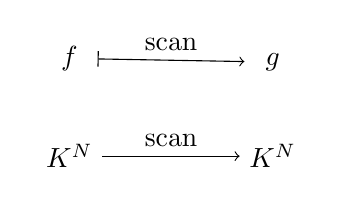
\begin{tikzpicture}
  \matrix (m) [matrix of math nodes, row sep=2em, column sep=5em, minimum width=2em]
  {
    f & g \\
    K^N & K^N \\
};
  \path[|->]
  (m-1-1) edge node [auto] {$\text{scan}$} (m-1-2);
\path[->]
  (m-2-1) edge node [auto] {$\text{scan}$} (m-2-2)
  ;
  \end{tikzpicture}
    \end{equation}
  with
  \textbf{inclusive scan} defined as
  \begin{equation}
\boxed{ g(i) = \bigoplus_{j=0}^i f(j) }
    \end{equation}
  and \textbf{exclusive scan} defined as 
  \begin{equation}
    \boxed{
      g(i) = \begin{cases} \bigoplus_{j=0}^{i-1}f(j) & \text{ if } i \geq 1 \\
        1 & \text{ if } i = 0 \end{cases}
    }
    \end{equation}
  
  \end{definition}



cf. \href{https://classroom.udacity.com/courses/cs344/lessons/86719951/concepts/880351220923#}{Hillis Steele Scan}

\subsubsection*{Hillis/Steele inclusive scan}

Let $\begin{aligned} & \quad \\
  & f \in K^N \, \qquad \, N \in \mathbb{Z}^+ \\
  & f(j) \in K \, \qquad \, j \in \lbrace 0 \dots N-1 \rbrace \end{aligned}$

Consider step $i=0$.

For $g_i \in K^N$, $\forall \, i\in \lbrace 0 , \dots , \log_2{N}-1 \rbrace$, 

Doing the first 3 steps,
\[
\begin{aligned}
  & g_0(j) = \begin{cases} f(j) + f(j-2^0) & \text{ if } j \geq 1 \\
    f(j) & \text{ if } j < 1 \end{cases} \\
  & g_1(j) = \begin{cases} g_0(j) + g_0(j-2^1) & \text{ if } j \geq 2^1 \\
    g_0(j) & \text{ if } j < 2^1 \end{cases} \\
  & g_2(j) = \begin{cases} g_1(j) + g_1(j-2^2) & \text{ if } j \geq 2^2 \\
    g_1(j) & \text{ if } j < 2^2 \end{cases} \\
\end{aligned}
\]
Thus
\[
   g_i(j) = \begin{cases} g_{i-1}(j) + g_{i-1}(j-2^i) & \text{ if } j \geq 2^i \\
    g_{i-1}(j) & \text{ if } j < 2^i \end{cases} \\
\]

Now do the following induction cases:
\[
\begin{aligned}
  & g_{\log_2{N}}(0) = f(0) \\ 
  & g_{\log_2{N}}(1) = g_0(1) = f(1) + f(0) \\
  & g_{\log_2{N}}(2) = g_1(2) = g_0(2) + g_0(0) = f(2)+f(1) + f(0) \\
  & g_{\log_2{N}}(3) = g_1(3) = g_0(3) + g_0(1) = f(3)+f(2)+f(1)+f(0)  \\
\end{aligned}
\]
So generalize to the induction case:
\[
g_{ \log_2{N} }(j) = \bigoplus_{i=0}^j f(i)
\]
Then one would check the induction step for a number of cases, whether $j$ was greater or smaller or equal to $2^{ \log_2{N}}$.  

To summarize for the Hillis/Steele inclusive scan,
\begin{equation}
  \boxed{ \begin{gathered}
      \forall \, i \in \lbrace 0 ,1 , \dots , \log_2{N} | 2^i < N \rbrace \\ 
      g_{i-1}(j) = f(j) \qquad \, \forall \, j \in \lbrace 0 \dots N-1 \rbrace \\
      g_i(j) = \begin{cases}
        g_{i-1}(j) + g_{i-1}(j-2^i) & \text{ if } j \geq 2^i \\
        g_{i-1}(j) & \text{ if } j < 2^i \end{cases}
      \end{gathered}
  }
  \end{equation}
i.e.
\begin{equation}
  \boxed{ \begin{gathered}
      \forall \, i \in \lbrace 0 ,1 , \dots , \lfloor \log_2{N} \rfloor | 2^i < N \rbrace \\ 
      g_{-1}(j) = f(j) \qquad \, \forall \, j \in \lbrace 0 \dots N-1 \rbrace \\
      g_i(j) = \begin{cases}
        g_{i-1}(j) + g_{i-1}(j-2^i) & \text{ if } j \geq 2^i \\
        g_{i-1}(j) & \text{ if } j < 2^i \end{cases}
      \end{gathered}
  }
  \end{equation}


Implementation is CUDA C/C++:  consider $k_x:= i_x + M_xj_x \in \lbrace 0,1, \dots , L_x\rbrace$, $L_x \in \mathbb{Z}^+$, with the formula
\[
N_x := \frac{L_x + M_x-1}{M_x}
\]
that'll give us \verb|blockDim.x|.

$\forall \, i \in \lbrace 0 ,1\dots \log_2{k_x} \rbrace$ (or $k_x <2^i$),
\[
g_i(k_x) = g_{i-1}(k_x) + g_{i-1}(k_x-2^i)  
\]


For \emph{(inclusive) scan},

step : $O(\log{ n } )$ \\
work : $O(n^2)$ \\

For \emph{ Hillis/Steele },

step : $O(\log{ n } )$ \\
work : $O(n \log{n} )$ \\

(more step efficient)

For \emph{B}

cf. \href{https://classroom.udacity.com/courses/cs344/lessons/86719951/concepts/880351210923#}{Inclusive Scan Revisited}, \href{https://classroom.udacity.com/courses/cs344/lessons/86719951/concepts/873907230923#}{Hillis Steele vs Blelloch Scan},\href{https://classroom.udacity.com/courses/cs344/lessons/86719951/concepts/880351220923#}{Hillis Steele Scan},


\subsection{Blelloch scan}
cf. \href{https://classroom.udacity.com/courses/cs344/lessons/86719951/concepts/880351240923#}{Blelloch Scan}

\subsubsection{Blelloch scan, reduce, 1st part, up sweep } 

My development: consider the most basic cases.  So for $f\in K^N$,
\[
\begin{gathered}
  \begin{gathered}
    i \in \lbrace 0 , 1 , \dots N -1 \rbrace   \\
    2j, \qquad \, j \in \lbrace 1 , 2 , \dots, \lfloor N/2 \rfloor  \rbrace  \\
    i = 2j - 1  \\
    2^2 j - 1 , \qquad \, j\in \lbrace 1 ,2, \dots , \lfloor N/2^2 \rfloor \rbrace \\
    2^3j -1 , \qquad \, j \in \lbrace 1  , 2 , \dots , \lfloor N/2^3 \rfloor \rbrace 
    \end{gathered}
\qquad \quad \, \begin{gathered}
  N = 8 \qquad \, i \in \lbrace 0 , 1 , \dots, 8  - 1 = 7 \rbrace  \\
  2j \in \lbrace 2 ,4 , 6 , 8 \rbrace, \, j \in \lbrace 1,2,3,4 \rbrace \\ 
  i = 2j - 1 \in \lbrace 1,3,5,7 \rbrace \\
  j \in \lbrace 1 , 2 \rbrace , \qquad \, i \in \lbrace 3 , 7 \rbrace \\
  j\in \lbrace 1 \rbrace , \qquad \, i \in \lbrace 7 \rbrace
  \end{gathered}
\end{gathered}
\]

Then $\forall \, k = \lbrace 1, 2, \dots , \lfloor \log_2{ N} \rfloor \rbrace$,
\[
\begin{aligned}
  & k =1 , \qquad \, f_{\text{out}}[i] = \begin{cases} f[i] + f[i-1] & \text{ if } i = 2j - 1 , \, j \in \lbrace 1,2, \dots \lfloor N/2 \rfloor \rbrace \\
    f[i] & \text{ otherwise } \end{cases} \\
    & k =2 , \qquad \, f_{\text{out}}[i] = \begin{cases} f[i] + f[i-2^{(k-1)}] & \text{ if } i = 2^2j - 1 , \, j \in \lbrace 1,2, \dots \lfloor N/2^2 \rfloor \rbrace \\
    f[i] & \text{ otherwise } \end{cases} \\ 
  & k \phantom{=1}  , \qquad \, f_{\text{out}}[i] = \begin{cases} f[i] + f[i-2^{(k-1)}] & \text{ if } i = 2^kj - 1 , \, j \in \lbrace 1,2, \dots \lfloor N/2^k \rfloor \rbrace \\
    f[i] & \text{ otherwise } \end{cases}
\end{aligned}
\]

Thus
\begin{definition}[Blelloch scan: 1st part that's reduce, i.e. up sweep]
  \[
\forall \, k \in \lbrace 1, 2, \dots \lfloor \log_2{N} \rfloor \rbrace
\]
\begin{equation}
  f_{\text{out}}[i] = \begin{cases} f[i] + f[i-2^{(k-1)}] & \text{ if } i = 2^kj - 1 , \, j \in \lbrace 1,2, \dots \lfloor N/2^k \rfloor \rbrace \\
    f[i] & \text{ otherwise } \end{cases}
  \end{equation}
for
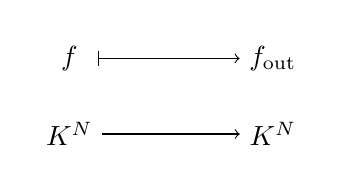
\begin{tikzpicture}
  \matrix (m) [matrix of math nodes, row sep=1.2em, column sep=5em, minimum width=2em]
  {
    f & f_{\text{out}} \\
    K^N & K^N \\
};
  \path[|->]
  (m-1-1) edge node [auto] {$\text{}$} (m-1-2);
\path[->]
  (m-2-1) edge node [auto] {$\text{}$} (m-2-2)
  ;
  \end{tikzpicture}
  \end{definition}

\subsubsection{Blelloch scan, down sweep part}

Now consider the down sweep.  First, importantly, set the ``last'' element in the array, entry number $\lfloor \log_2{N} \rfloor$, $N$ being the length of the array, to the identity element of $K$.  

I'll present the first few induction steps explicitly, and the general form can be guessed from there.


\[
\forall \, k \in \lbrace \lfloor \log_2N \rfloor , \lfloor \log_2N \rfloor -1, \dots , 2, 1 \rbrace
\]
If $i = 2^kj - 1$, \, $j\in \lbrace 1,2, \dots , \lfloor N/2^k \rfloor \rbrace$, for e.g. $k = \lfloor \log_2N \rfloor$,
\[
\begin{aligned}
  & f_{\text{out}}[i-2^{(k-1)}] = f[i] \\ 
  & f_{\text{out}}[i] = f[i] + f[i-2^{(k-1)} ]
  \end{aligned}
\]
For $k = \lfloor \log_2 N \rfloor -1$, e.g. $k=3-1=2$, then for this exmaple, \\
e.g. $i=2^kj-1 = 4j-1$; $j\in \lbrace 1,2 \rbrace$, $i\in \lbrace 3,7\rbrace$,
\[
\begin{aligned}
  & f_{\text{out}}[i] = f[i] + f[i-2] \\ 
  & f_{\text{out}}[i-2] = f[i]
\end{aligned}
\]

Thus, in general,
\begin{definition}[Blelloch scan: down sweep step]
\[
\forall \, k \in \lbrace \lfloor \log_2N \rfloor , \lfloor \log_2N \rfloor -1, \dots , 2, 1 \rbrace
\]
\begin{equation}
\begin{cases}
\begin{aligned} &   f_{\text{out}}[i] := f[i] + f[i-2^{(k-1)}] \\ 
  & f_{\text{out}}[i-2^{(k-1)}] := f[i] \end{aligned} & \text{ if } i = 2^kj-1 \text{ and } j \in \lbrace 1,2, \dots , \lfloor N/2^k \rfloor \rbrace \\
f_{\text{out}}[i] := f[i]  & \text{ otherwise}
  \end{cases}
\end{equation}
\end{definition}







cf.  \href{https://classroom.udacity.com/courses/cs344/lessons/86719951/concepts/907138050923#}{Problem Set 3} 

\subsubsection*{Histogram Equalization}

\begin{enumerate}
\item Map
\item Reduce
\item Scatter
\item Scan
  \end{enumerate}


\subsection{Reduce, Parallel Reduction}

I will expound upon the excellent article from Mark Harris, ``Optimizing Parallel Reduction in CUDA''.  cf. \href{http://developer.download.nvidia.com/compute/cuda/1.1-Beta/x86_website/projects/reduction/doc/reduction.pdf}{\emph{Optimizing Parallel Reduction in CUDA}, Mark Harris} : \url{http://developer.download.nvidia.com/compute/cuda/1.1-Beta/x86_website/projects/reduction/doc/reduction.pdf}


\subsection{Unit 4}

\subsection{Unit 5}

\subsubsection{Occupancy}

cf. \href{https://classroom.udacity.com/courses/cs344/lessons/109244577/concepts/1118375690923#}{Occupancy Part 1}

Each SM (streaming multi-processor) has a limited number of
\begin{itemize}
\item thread blocks (so there's a maximum number of thread blocks, e.g. 8)
\item threads (so there's a maximum number of threads, e.g. 1536-2048)
\item registers for all threads (every thread takes a certain number of registers, and there's a maximum number of registers for all the threads, e.g. 65536)
\item bytes of shared memory
  \end{itemize}

cf. \href{https://classroom.udacity.com/courses/cs344/lessons/109244577/concepts/1110067030923}{Quiz: Occupancy Part 2}

Compile and run \verb|deviceQuery_simplified.cpp| (can be found in Lesson 5 Code Snippets).

Look at

\begin{itemize}
\item Total amount of shared memory per block
\item Maximum number of threads per multiprocessor  
\item Maximum number of threads per block  
\end{itemize}
  
For Luebke's laptop, it's 49152 bytes, 2048, 1024 respectively, and 65536 total registers available per block.  

\subsubsection{Thread Divergence}

cf. \href{https://classroom.udacity.com/courses/cs344/lessons/109244577/concepts/1109210790923#}{Quiz: Swith Statements and Thread Divergence}

Threads in warp is 32 (check hardware, usually this is the case for modern GPUs).  Only 32 threads in a warp, i.e. $2^5$.

CUDA assigns thread IDs to warps:

\begin{itemize}
\item $x$ varies fastest
\item $y$ varies slower
\item $z$ varies slowest
\end{itemize}
warp assignment, consider $(M_x,M_y,M_z) \equiv $ number of threads in a single thread block, in each dimensional direction.

Consider
\[
\begin{aligned}
  & i_x \in \lbrace 0 , \dots , M_x - 1 \rbrace \\ 
  & i_y \in \lbrace 0 , \dots , M_y - 1 \rbrace
  \end{aligned}
\]

If $M_x/2^5 \in \mathbb{Z}^+$, i.e. $M_x/2^5\geq 1$, then threads in $x$-direction are in warps that branch (go to same case in if-else, or switch, case statement in kernel) to same case.

\subsubsection{Problem Set 5}

2. One Basic Strategy

A. Sort the Data, into bins, sort the input data, into coarse bins

B. use threads, compute local histogram, use each thread block, to compute local histogram

c. concatenate

e.g.

Consider

$J = $ total number of coarse bins, $J\in \mathbb{Z}^+$.

$j\in \lbrace 0 \dots J-1 \rbrace$, e.g. $J=10$.

$K = $ total number of bins,

$k\in \lbrace 0 \dots K-1 \rbrace$,  e.g. $K = 100$

The condition is that $J< K$

For each thread block,

\subsubsection{Parallel radix sort}

cf. look at, in the directory 
\url{http://www.compsci.hunter.cuny.edu/~sweiss/course_materials/csci360/lecture_notes/}
for the parallel radix sort implementation called \verb|radix_sort_cuda.cc|.

Let $M_x \in \mathbb{Z}^+$ represent
\begin{equation}
  M_x \leftrightarrow \verb|blockDim.x |
\end{equation}

\begin{equation}
  j_x \in \lbrace 0 , 1 , \dots M_x -1 \rbrace \leftrightarrow \verb| blockIdx.x |
\end{equation}

$\forall \, j_x \in \lbrace 0 , 1 \dots , M_x - 1\rbrace $, $j_x $ denote which thread block we are in.

$j_x$ also corresponds to the so-called coarse bin id.  


\subsection{Lesson 6.1 - Parallel Computing Patterns Part A}

\subsubsection{parallel All Pairs $N$-body}

cf. \href{https://classroom.udacity.com/courses/cs344/lessons/116611037/concepts/1198442170923#}{Quiz: All Pairs $N$-Body}

From Arnold, Kozlov, Neishtadt, and Khukhro (2006) \cite{AKNK2006}, given $N$-bodies $\lbrace 1,2 \dots N\rbrace \subset \mathbb{Z}^+$.
\[
(\mathbf{r}_1, M_1), (\mathbf{r}_2, M_2), \dots (\mathbf{r}_N, M_N) \qquad \, \mathbf{r}_i \in \mathbb{R}^d
\]
With the force acting upon the $i$th body (``destination'') due to the $j$th body (``source''), $\mathbf{F}_{ij}$,
\begin{equation}
  \mathbf{F}_{ij} = - \frac{\gamma M_i M_j}{ |\mathbf{r}_{ij} |^3 } \mathbf{r}_{ij} \qquad \, \text{ with } \mathbf{r}_{ij} := \mathbf{r}_j - \mathbf{r}_i
\end{equation}
$N(N-1)$ are the number of (unordered) pairs, for
\begin{equation}
\mathbf{F}_i = \sum_{i\neq j} \mathbf{F}_{ij}
\end{equation}
with $\mathbf{F}_i$ denoting the force acting upon $i$th body, $N-1$ computations
\begin{equation}
\mathbf{F}_i =\sum_{i\neq j} \frac{- \gamma M_i M_j }{ |\mathbf{r}_{ij} |^3 } \mathbf{r}_{ij} = -\gamma M_i \sum_{i\neq j} \frac{ M_j}{ |\mathbf{r}_{ij} |^3 } \mathbf{r}_{ij}
\end{equation}

Consider another pairwise computation:
\begin{equation}
  W(\lambda) = \sum_{i=1}^m \lambda_i - \frac{1}{2} \sum_{i,j=1}^m y^{(i)} y^{(j)} \lambda_i\lambda_j K(X^{(i)}, X^{(j)})
\end{equation}
Define, for (writing) convenience,$f_1(\lambda) = -\frac{1}{2} \sum_{i,j=1}^m y^{(i)} y^{(j)} \lambda_i\lambda_j K(X^{(i)}, X^{(j)})$.  









cf. \href{https://classroom.udacity.com/courses/cs344/lessons/116611037/concepts/1198442170923#}{Quiz: How To Implement Dense $N$-Body as Simply As Possible}

For a single body, say $I$th body $(\mathbf{r}_I, M_I)$, consider $\mathbf{F}_i =\sum_{i\neq j} \mathbf{F}_{ij} \qquad \, \forall \, i = 1, \dots N$.  \\
$j=I$ once, $\forall \, i = 1, \dots N$ and $i\neq I$ ($I$th body as a ``source'') $N-1$ times.  \\
$i=I$ once, in $\mathbf{F}_I=\sum_{i\neq j} \mathbf{F}_{Ij}$, we'll need $(\mathbf{r}_I, M_I)$, to calculate $\mathbf{F}_{Ij}$, $N-1$ times.

If all $N^2$ force computations, go to global memory, the number of times we'd fetch each element, as a function of $N$ is $\boxed{ 2(N-1) }$.  

cf. \href{https://classroom.udacity.com/courses/cs344/lessons/116611037/concepts/1198442190923#}{Quiz: Dividing $N$ by $N$ Matrix Into Tiles}  

Consider $N\times N$ matrix $A$, $A\in \text{Mat}_{\mathbb{K}}(N_x,N_y)$.

Consider dividing it by tiles, calculate each tile, a tile of $P_x \times P_y$.

So there are $\frac{N_xN_y}{P_xP_y}$ tiles overall.

For this particular problem, and in general, a problem involving pairwise \emph{combination} out of a given set, say $N$ bodies, consider $N^2$ possible pairs total.  Then this all $N$-body algorithm idea is to transform all these combinations $N^2$, into a matrix, and so $N_x=N_y=N$, $P_x=P_y=P$.

\begin{equation}
\begin{gathered}
  \mathbf{F}_i = \sum_{i\neq j}^N \mathbf{F}_{ij} = \sum_{t=0}^{\frac{N}{P}-1} \sum_{ \substack{ j=0 \\ Pt+j\neq i  }  }^{P-1} \mathbf{F}_{i(Pt+j)} \equiv \sum_{t=0}^{\frac{N}{P}-1} \mathbf{F}_i^{(t)}
  \end{gathered}
\end{equation}
$2P$ fetches per tile, instead of $2P^2$, if $\forall \, $ tile, store the $P$ elements into shared memory.

cf. \href{https://classroom.udacity.com/courses/cs344/lessons/116611037/concepts/1168851160923}{Using on $P$ threads}

Consider this computation:
\begin{equation}
  \mathbf{F}_i^{(t)} = \sum_{ \substack{ j=0 \\ pt+j\neq i } }^{P-1} \mathbf{F}_{i(Pt+j)} \qquad \, i=0\dots N-1, t=0,1,\dots \frac{N}{P}-1
\end{equation}
For
\[
i \Longleftrightarrow i_x + M_x j_x, \qquad \, \begin{aligned}
  & i_x \equiv \verb|threadIdx.x| \in \lbrace 0 ,1 \dots M_x- 1 \rbrace \\
  & j_x \equiv \verb|blockIdx.x| \in \lbrace 0 ,1 ,\dots N/M_x-1 \rbrace \\
  & M_x = P \end{aligned}
\]
So $\forall \, (i_x,j_x)$, $(i_x,j_x)$ representing a single thread, this single thread will be responsible for computing
\[
\mathbf{F}_i^{(t)} =\sum_{j=0}^{P-1} \mathbf{F}_{i(Pt+j)}
\]
, as opposed to only computing $\mathbf{F}_{i(Pt+j)}$ only.  


The pseudocode that Owens gives in \href{https://classroom.udacity.com/courses/cs344/lessons/116611037/concepts/1168851160923}{Using On P Threads, Lesson 6.1} is the following:

\begin{lstlisting}
  __device__ float3
  tile_calculation(Params myParams, float3 force) {
    int i;
    extern __shared__ Params[] sourceParams;
    for (i=0; i<blockDim.x; i++) {
      force += bodyBodyInteraction(myParams, sourceParams[i]);
    }
    return force;
  }
  \end{lstlisting}


  
\subsection{Final for Udacity cs344}

\subsubsection{Quiz: Final - Question 7}

cf. \url{https://classroom.udacity.com/courses/cs344/lessons/2133758814/concepts/1421890260923#}

Second question:

What is the ratio (expressed as a percentage) between kernel that uses more memory bandwidth and the kernel that uses less?

For both parts of this question, here's how to approach it.

Consider a stencil of radius $\text{RAD} \equiv R = 2$.  So the filter-width in 1-dimension for this 2-dimensional stencil is
\[
\text{filterwidth} \equiv W  = 2 \cdot \text{RAD}  +1 = 5
\]
$W^2$ multiples, and $W^2-1$ adds.

$\forall \, k \in K$, a (single) pixel of greyscale image, $k\in \lbrace 0 , 1, \dots N-1 \rbrace$, \\

Consider the threads per block configuration (i.e. a single thread block).

Let $M \equiv M_x M_y = 1024$ in both, either, case, i.e. totla number of threads per block is 1024.

Consider $\begin{aligned} & \quad \\
  & (M_x,M_y) = (1024, 1) \text{ vs. } \\ 
  & (M_x,M_y) = (32, 32) \text{ vs. } \end{aligned}$,  \\
Correspoding to
\[
\verb|dim3| M_i(M_x,M_y)
\]
for
\[
\text{smooth} \verb| <<<  , M_i >>> |( \verb|v_new|, v) ;
\]

The big idea is that we have a tile of input data we want to load into 2-dimensional shared memory.  It is of size
\begin{equation}
  (M_x + 2R) (M_y + 2R)
\end{equation}
Compare this quantity to when $(M_x,M_y) = (1024,1)$ vs. when it's $(32,32)$.
\[
\begin{gathered}
  (1024 +4 )(1+4) / (32 +4)*(32 +4) = \boxed{ 3.966 }
  \end{gathered}
\]
This is the ratio between the kernel with more memory bandwidth and the kernel with less memory bandwidth.  

Note, in the Udacity forum, \href{https://discussions.udacity.com/t/final-updated-questions-7-8/88801/2}{Final: Updated Questions 7 \& 8}, jlmayfield gave the hint to consider those stencil halo cells or what I call the radius $R$ of the stencil, as this stencil is $5x5$.    

\subsubsection{Quiz: Final - Question 8}

cf. \href{https://classroom.udacity.com/courses/cs344/lessons/2133758814/concepts/1421890280923}{Quiz:Final - Question 8}

$32 \times 32 $ block, but consider
\begin{itemize}
\item 4x storage per SM
\item 4x registers
\item 4x shared memory
  \end{itemize}
now 64 x 64 since, in each dimension, 2x the global memory available ($2\times 2 = 4$).  

Express, in decimals, what the speedup is on this new GPU.

Here's how I approached this problem:  

so in a single thread block, we can have a much larger tile with inputted data to reside in shared memory and so we can process a much larger tile of inputted data in a single thread block:
\begin{equation}
\begin{gathered}
  (M_x + 2R)(M_y + 2R) = ( 64 + 2*2)*(64 + 2*2) = 4624
\end{gathered}
\end{equation}
instead of when $(M_x,M_y)=(32,32)$.

Not only that 4x of shared memory, 4x storage per SM, but also \emph{4x registers}.  More registers for the threads, more a thread can be doing something and not have to wait for another thread (or even to hop on to another thread if the thread itself doesn't have enough registers).  More throughput, by 4x.

\begin{equation}
\begin{gathered}
  (64 + 2R)(64 + 2R) * 4 /   (32 + 2R)(32 + 2R) = \boxed{ 14.27 \text{ or } 14.0 }
  \end{gathered}
  \end{equation}


There was confusion about Final - Question 8 in the Udacity Forums: \href{https://discussions.udacity.com/t/final-question-8/46261}{Final - Question 8}

\subsubsection{Quiz: Final - Question 9}

cf. \url{https://classroom.udacity.com/courses/cs344/lessons/2133758814/concepts/1389566540923}

If I want to run the maximum number of threads possible that are all resident on an SM (streaming multiprocessor) at the same time, each thread must use no more than, \emph{how many}, registers?

\begin{equation}
\boxed{ 32  \text{ registers } }
  \end{equation}





This is obtained by looking at \url{http://en.wikipedia.org/wiki/CUDA} (this was given) and look for
\begin{itemize}
\item ``Maximum number of resident threads per multiprocessor'': 2048 for Compute ability (version) 3.5.
\item 
  \end{itemize}

\href{https://discussions.udacity.com/t/final-exam-question-9-confusion/88637}{Final Exam Question 9 confusion}

\url{https://discussions.udacity.com/t/final-exam-question-9-confusion/88637}


\subsubsection{Quiz: Final - Question 11}

Maximum number of blocks resident on the same SM, what is the maximum number of threads $/$ block that we can have?

This is obtained by looking at \url{http://en.wikipedia.org/wiki/CUDA} (this was given) and look for
\begin{itemize}
\item ``Maximum number of resident blocks per multiprocessor'': 16 for Compute ability (version) 3.5.
\item ``Maximum number of resident threads per multiprocessor'': 2048 for Compute ability (version) 3.5.
  \end{itemize}

The answer is
\begin{equation}
\begin{gathered}
\boxed{ 2048 / 16 = 128 }
  \end{gathered}
  \end{equation}
Since we take max. number of resident threads per SM, 2048, but the condition is using the max. number of resident blocks per SM, so, divide by 16.  

\subsubsection{Quiz: Final - Question 12; Fast ``compact'' primitive}

Consider the \emph{Fast `` compact'' primitive}.

\begin{enumerate}
\item sum up the no. of ``T'' flags
\end{enumerate}
e.g. warp of size 4 (only to make it easy to understand), (4 warps of 4 flags each), e.g.
\[
TFTF / FTFT / TTTT / tfff
\]

\begin{enumerate}
\item \[
2 / 2 / 4 / 1 
  \]
  \end{enumerate}

Let warp size $W=2^n$; $n\in \mathbb{Z}^+$, e.g. $n=5$ for $W=32$.

Given shared memory $s\in (\mathbb{Z}^+)^W$,
\[
\forall \, i \in \lbrace W/2, W/4 , \dots | i > 0 \rbrace
\]
For given \verb|ARRAY_SIZE = 32 = | $M_x$ so $M_x =W$ (thread block size is equal to warp size in this case).

Keep in mind, even in a \verb|__device__| function, we've got \textbf{access} to
\[
\begin{gathered}
  i_x \equiv \verb|threadIdx.x| \in \lbrace 0 , 1\dots, M_x - 1\rbrace
\end{gathered}
\]
(and so on).

$i_x < i$, i.e. $\forall \, i_x < i$ and $i_x \in \lbrace 0 , 1\dots M_x - 1\rbrace$

\[
s[i_x] = s[i_x] + s[i_x + i]
\]
e.g. $i=W/2$
\[
i_x \in \lbrace 0 ,1 \dots, \frac{W}{2} - 1\rbrace
\]
$i = W/4$
\[
i_x \in \lbrace 0,1 \dots \frac{W}{4} -1 \rbrace
\]

\[
s[i_x] = s[i_x] + s[i_x+1] \Longrightarrow \begin{aligned}
& s[0] = s[0] + s[\frac{W}{2} ] + s[0 + \frac{W}{4} ] \\ 
  & \vdots \\
  & s[\frac{W}{4} -1 ] = s[ \frac{W}{4}-1] + s[\frac{3W}{4} - 1] + s[\frac{W}{2} -1]
  \end{aligned}
\]
So by induction, for $i=1$, $i_x=0$.
\[
s[0] = \sum_{j=0}^{W-1} s[j]
\]
which is the desired result (!!!).

Code answer uploaded here: \href{https://github.com/ernestyalumni/cs344/blob/master/Final/Q12warpreduce_shared.cu}{Q12warpreduce shared.cu} or here \href{https://github.com/ernestyalumni/cs344/blob/master/Final/warpreduce/part_a/warpreduce.cu}{warpreduce.cu}





\section{Pointers in C; Pointers in C categorified (interpreted in Category Theory)}

Suppose $v\in \text{ObjData}$, category of data \textbf{Data}, \\
\phantom{ Suppose} e.g. $v\in \text{Int} \in \text{Obj}\mathbf{\text{Type}}$, category of types $\mathbf{\text{Type}}$.

\[
\begin{aligned}
  & \text{Data}  \xrightarrow{ \& } \text{Memory}  \\
  & v \overset{\&}{\mapsto} \& v 
\end{aligned}
\]
with address $\& v \in $ Memory.

With \\
\phantom{With } assignment $pv = \& v$,
\[
\begin{aligned}
  & pv \in \text{Obj}\text{pointer}, \, \text{ category of pointers, pointer} \\ 
  & pv \in \text{Memory} \qquad \, (\text{i.e. not $pv \in \text{Dat}$, i.e. $pv \notin \text{Dat}$})
\end{aligned}
\]

\[
\text{ pointer } \ni pv \overset{ * }{ \mapsto } *pv \in \text{Dat}
\]

\[
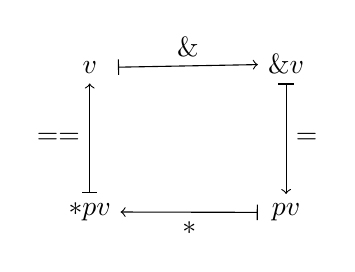
\begin{tikzpicture}
  \matrix (m) [matrix of math nodes, row sep=4em, column sep=5em, minimum width=2em]
  {
    v & \& v \\
    *pv & pv \\
};
  \path[|->]
  (m-1-1) edge node [auto] {$\&$} (m-1-2)
  (m-1-2) edge node [right] {$=$} (m-2-2)
  (m-2-2) edge node [auto] {$*$} (m-2-1)
  (m-2-1) edge node [left] {$==$} (m-1-1)
  ;
  \end{tikzpicture}
\qquad \, 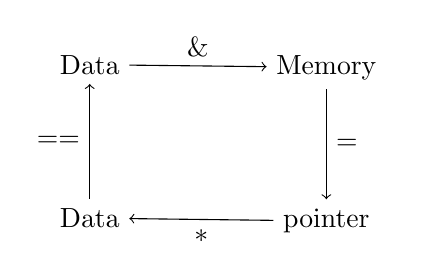
\begin{tikzpicture}
  \matrix (m) [matrix of math nodes, row sep=4em, column sep=5em, minimum width=2em]
  {
    \text{Data} & \text{Memory} \\
    \text{Data} & \text{pointer} \\
};
  \path[->]
  (m-1-1) edge node [auto] {$\&$} (m-1-2)
  (m-1-2) edge node [right] {$=$} (m-2-2)
  (m-2-2) edge node [auto] {$*$} (m-2-1)
  (m-2-1) edge node [left] {$==$} (m-1-1)
  ;
  \end{tikzpicture}
\]

Examples.  Consider \verb|passfunction.c| in Fitzpatrick \cite{Fitz}.

Consider the type \verb|double|, \verb|double| $\in \text{Obj}\text{Types}$.  \\
\phantom{ Consider } $\text{fun1, fun2} \in \text{Mor}\text{Types} \qquad \, \text{ namely }$ \\
\phantom{ Consider } $\text{fun1, fun2} \in \text{Hom}(\text{double},\text{double}) \equiv \text{Hom}_{\text{Types}}(\text{double},\text{double})$

Recall that
\[
\begin{aligned}
  & \text{ pointer } \xrightarrow{ * } \text{ Dat } \\ 
  & \text{ pointer } \xrightarrow{ \& } \text{ Memory }
\end{aligned}
\]
$*, \&$ are functors with domain on the category pointer.

Pointers to functions is the ``extension'' of functor $*$ to the codomain of $\text{Mor}\text{Types}$:

\[
\begin{aligned}
  & \text{ pointer} & \xrightarrow{ * } \text{Mor}\text{Types} \\ 
  & \text{ fun1 } & \overset{*}{ \mapsto } *\text{fun}1 \in \text{Hom}_{\text{Types}}(\text{double},\text{double})
  \end{aligned}
\]

\[
 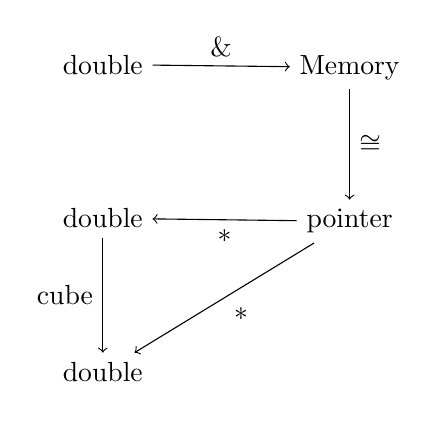
\begin{tikzpicture}
  \matrix (m) [matrix of math nodes, row sep=4em, column sep=5em, minimum width=2em]
  {
    \text{double} & \text{Memory} \\
    \text{double} & \text{pointer} \\
    \text{double} & \\ 
  };
  \path[->]
  (m-1-1) edge node [auto] {$\&$} (m-1-2)
  (m-1-2) edge node [right] {$\cong$} (m-2-2)
  (m-2-2) edge node [auto] {$*$} (m-2-1)
  edge node [auto] {$*$} (m-3-1)
  (m-2-1) edge node [left] {$\text{cube}$} (m-3-1)
  ;
 \end{tikzpicture} \qquad \qquad \,
  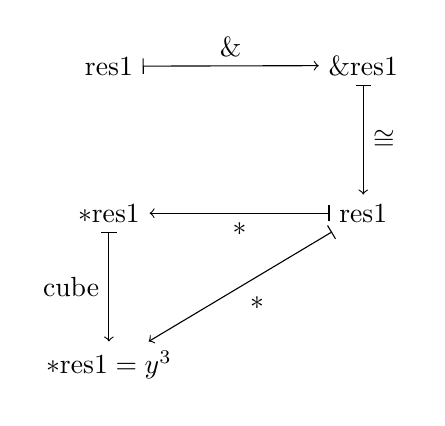
\begin{tikzpicture}
  \matrix (m) [matrix of math nodes, row sep=4em, column sep=5em, minimum width=2em]
  {
    \text{res1} & \&\text{res1} \\
    *\text{res1} & \text{res1} \\
    *\text{res1} = y^3 & \\ 
  };
  \path[|->]
  (m-1-1) edge node [auto] {$\&$} (m-1-2)
  (m-1-2) edge node [right] {$\cong$} (m-2-2)
  (m-2-2) edge node [auto] {$*$} (m-2-1)
  edge node [auto] {$*$} (m-3-1)
  (m-2-1) edge node [left] {$\text{cube}$} (m-3-1)
  ;
  \end{tikzpicture}
\]

It's unclear to me how \verb|void cube| can be represented in terms of category theory, as surely it cannot be represented as a mapping (it acts upon a functor, namely the $*$ functor for pointers).  It doesn't return a value, and so one cannot be confident to say there's explicitly a domain and codomain, or range for that matter.

But what is going on is that
\[
\begin{gathered}
  \text{ pointer }, \text{ double } , \text{ pointer } \xrightarrow{ \text{ cube } } \text{ pointer }, \text{ pointer } \\ 
  \text{fun}1, x , \text{res}1 \overset{\text{cube}}{\mapsto} \text{fun}1, \text{res}1
\end{gathered}
\]
s.t. $*\text{res}1 = y^3=(*\text{fun}1(x))^3$


So I'll speculate that in this case, \verb|cube| is a functor, and in particular, is acting on $*$, the so-called deferencing operator:
\[
\begin{gathered}
  \text{ pointer } \xrightarrow{ * } \text{float} \in \text{Data} \\
  \text{ res}1 \overset{*}{\mapsto} *\text{res}1
\end{gathered} \xrightarrow{ \text{ cube } } \begin{gathered}
  \text{ pointer } \xrightarrow{ \text{cube}(*) } \text{float} \in \text{Data} \\
  \text{ res}1 \overset{\text{cube}(*)}{\mapsto} \text{cube}(*\text{res}1)=y^3
\end{gathered}
\]

cf.  Arrays, from Fitzpatrick \cite{Fitz}

\[
\text{Types} \xrightarrow{ \text{ declaration } } \text{arrays}
\]
If $x\in \text{Obj}\text{arrays}$,
\[
\& x[0] \in \text{Memory} \xrightarrow{ == } x \in \text{ pointer } (\text{to 1st element of array})
\]


cf. Section 2.13 Character Strings from Fitzpatrick \cite{Fitz}

\begin{lstlisting}
  char word[20] = ``four''
  char *word = ``four''
\end{lstlisting}

cf. C$++$ extensions for C according to Fitzpatrick \cite{Fitz}
\begin{itemize}
\item simplified syntax to pass by reference pointers into functions
\item inline functions
\item variable size arrays \begin{lstlisting}
  int n;
  double x[n];
  \end{lstlisting}
\item complex number class
\end{itemize}



\section{Summary of Udacity cs344 concepts}

\subsection{Histogram}

Consider given input values (of observations).  \\
For $n$ observations, \\
For $i\in \lbrace 1,2, \dots n \rbrace \subset \mathbb{Z}^+$, $\equiv i \lbrace 0 , 1, \dots n-1 \rbrace \subset \mathbb{Z}^+$.

Consider $x[i] \in B\subset \mathbb{K}$, so $x\in B^n \subset \mathbb{K}^n$.

e.g. $\mathbb{K} = \mathbb{R}$, $B$ is a subset that we can make $K$ bins out of, i.e.
\[
B = \prod_{j=1}^K B_j \equiv \prod_{j=0}^{K-1}B_j
\]

e.g. $B$ is bounded interval of $\mathbb{R}$, i.e. $\begin{aligned} & \quad \\
  & \max{ B} < \infty \\
  & \min{ B } > -\infty \end{aligned}$

Then the \emph{histogram} $H$ is mapping from bins to \emph{number} of observations, i.e.
\begin{equation}
  \begin{aligned}
    & H:\lbrace 1 , 2, \dots K \rbrace \to \mathbb{N}^K \\ 
    & H(j) \in \mathbb{N} = \lbrace 0,1, \dots \rbrace
    \end{aligned}
  \end{equation}
s.t.
\begin{equation}
  \boxed{ n  = \sum_{j=1}^K H(j) }
\end{equation}
with $n$ being the total number of observations.

In the implementation of $x:\lbrace 1 , 2, \dots n \rbrace \to B \subset \mathbb{K}$,

this was simplified to
\[
x:\lbrace 1 , 2, \dots n \rbrace \to \lbrace 1,2, \dots K \rbrace \subset \mathbb{Z}
\]
meaning each observation value is \emph{itself} which bin the observation belongs to.

Otherwise, a separate ``binning'' operation is needed:
\begin{equation}
  \begin{aligned}
    & x: \lbrace 1 , 2, \dots n \rbrace \to & B \subset \mathbb{K} \to & \lbrace 1,2, \dots K \rbrace \\ 
    & i \mapsto & x[i]  \mapsto & \text{ if } B_{j-1} \leq x[i] < B_j , \text{ then return $j$ }
    \end{aligned}
  \end{equation}

\subsubsection{Histogram implementations; histogram references}

\href{https://github.com/ernestyalumni/cs344/tree/master/Problem%20Sets/Problem%20Set%205/histogram}{ernestyalumni/cs344/Problem Sets/Problem Set 5/histogram/}

  \url{https://github.com/ernestyalumni/cs344/tree/master/Problem%20Sets/Problem%20Set%205/histogram}




\part{Notes on \text{Professional CUDA C Programming}, Cheng, Grossman, McKercher}
cf. Cheng, Grossman, and McKercher (2014) \cite{CGM2014}
\section{CUDA Execution Model}
cf. Ch. 3.  CUDA Execution Model 

When kernel grid is launched, thread blocks of that kernel grid are distributed among available SMs for execution.  Once scheduled on SM, threads of a thread block execute concurrently only on that assigned SM.  

CUDA employs \emph{Single Instruction Multiple Thread (SIMT)} architecture to manage and execute threads in groups of 32 called \emph{warps}.  

All threads in warp execute same instruction at the same time.  Each thread has its own instruction address counter and register state, and carries out the current instruction on its own data.  Each SM partitions the thread blocks assigned to it into 32-thread warps that it then schedules for execution on available hardware resources.  

SIMT allows multiple threads in same warp to execute independently.  Even though all threads in a warps start together at the same program address, it's possible for individual threads to have different behavior.  


\subsubsection{GPU Core Versus CPU Core}  

\begin{itemize}
	\item CPU core, relatively heavy-weight, is designed for very complex control logic, optimizing latency $T$, namely $T(1)$, with $n_{\text{ops}}=1$.  
	\item GPU core, relatively light-weight, optimized for data-parallel tasks with simpler control logic, optimizing for throughput   
\end{itemize}
cf. pp. 8 of Cheng, Grossman, and McKercher (2014) \cite{CGM2014}

\emph{GPU capability}, described by 
\begin{itemize}
	\item number of CUDA cores  
	\item Memory size
\end{itemize}

\emph{GPU performance}, describe by 
\begin{itemize}
	\item \emph{Peak computational performance} $:=$ how many single-precision or double-precision floating point calculations that can be processed per second.  (gflops (billion floating-point operations per second) or tflops (trillion floating-point calculations per second)).  
	\begin{itemize}
		\item EY : 20170911 Peak computational performance $=$ (compute) throughput (???)
	\end{itemize}
	\item \textbf{Memory bandwidth} $:=$ ratio at which data can be read from or stored to memory; gigabytes per second, GB/s
\end{itemize}
cf. pp. 8 of Cheng, Grossman, and McKercher (2014) \cite{CGM2014}

CUDA kernels have no support for \emph{static} variables.  



cf. pp. 38 of Cheng, Grossman, and McKercher (2014) \cite{CGM2014}



\subsection{Understanding the Nature of Warp Execution; Warps and Thread Blocks}  

Once a thread block is scheduled to an SM, threads in thread block are further partitioned into warps.  A warp consists of 32 consecutive threads and all threads in a warp are executed in SIMT, i.e. all threads execute same instruction, and each thread carries out operation on its own private data.  

\subsubsection{Warp Divergence }
For example, consider the following statement:  
\begin{lstlisting}  
if (cond) {
...   
} else {
...
}
\end{lstlisting}

Suppose for 16 threads in a warp executing this code, \verb|cond| is \verb|true|, but for other 16 \verb|cond| is \verb|false|.  Then half of the warp will need to execute the instructions in the \verb|if| block, and the other half will need to execute the instructions in the \verb|else| block.  Threads in the same warp executing different instructions is referred to as \textbf{warp divergence.} 

If threads of a warp diverge, the warp serially executes each branch path, disabling threads that do not take that path.  

e.g. All threads within a warp must take both branches of the \verb|if ... then| statement.  If condition is \verb|true| for a thread, it executes the \verb|if| clause; otherwise, the thread stalls while waiting for that execution to complete.  




\section{Streams and Concurrency}  
cf. Ch. 6 Streams and Concurrency of  Chen, Grossman, and McKercher (2014) \cite{CGM2014}
\subsubsection{Introducing Streams and Events}
\begin{itemize}
	\item Functions in the CUDA API with \emph{synchronous behavior} block the host thread until they complete.  
	\item Functions in the CUDA API with \emph{asynchronous behavior} return control to host immediately after being called.  
\end{itemize}  
\subsubsection{CUDA Streams}
\begin{itemize}
	\item \emph{NULL stream}, default stream the kernel launches, implicitly declared, and data transfers use if you don't explicitly specify a stream.  
	\item \emph{non-null streams} explicitly created and managed; if you want to overlap different CUDA operations, you must use non-null streams.  
\end{itemize}
Consider 
\begin{lstlisting}
cudaMemcpy(...,cudaMemcpyHostToDevice);|
kernel<<<grid,block>>>(...);
cudaMemcpy(..., cudaMemcpyDeviceToHost);|
\end{lstlisting}
From device perspective, all 3 operations are issued to default stream, and executed in order they were issued.  Device has no awareness any other host operations performed.  
From host perspective, each data transfer is synchronous and forces idle host time while waiting for them to complete.  The kernel launch is \emph{asynchronous}, so host application almost immediately resumes execution afterwards.  
When performing an asynchronous data trasfer, you must use pinned (or non-pageable) host memory.  Pinned memory can be allocated using either \verb|cudaMallocHost| or \verb|cudaHostAlloc|:  
\begin{lstlisting}
cudaError_t cudaMallocHost(void **ptr, size_t size);
cudaError_t cudaHostAlloc(void **pHost, size_t size,unsigned int flags);
\end{lstlisting}
\part{More Parallel Computing}
\section{Matrix Multiplication, tiled, with shared memory}
Consider matrix multiplication:  
\[
\begin{aligned}
& A \in \text{Mat}_{\mathbb{K}}(N_i^A, N_j^A)  \\ 
& B \in \text{Mat}_{\mathbb{K}}(N_i^B, N_j^B)  \\
& C \in \text{Mat}_{\mathbb{K}}(N_i^C, N_j^C)  
\end{aligned}
\]
$AB=C$, 
\[
\begin{aligned}
& N_i^A = N_i^C \equiv N^A \\ 
& N_j^A = N_i^B \equiv N^B \\ 
& N_j^C = N_j^B \equiv N^C 
\end{aligned}
\]
\[
C_{ij} = A_{ik}B_{kj} = \sum_{k=1}^N A_{ik} B_{kj} \qquad \, \forall \, \begin{aligned} & \quad \\ 
& i=1,2,\dots N^A \\
& j = 1,2,\dots N^C \end{aligned}
\]
Consider, given \emph{block size} $M\in \mathbb{Z}^+$, 
\[
\begin{aligned}
& j_y = 0,1,\dots \frac{N^A}{M} - 1 \equiv \verb|blockIdx.y| =: j_I \\
& j_x = 0,1,\dots \frac{N^C}{M} -1 \equiv \verb|blockIdx.x| =: j_J 
\end{aligned}
\]
Given $A \in \text{Mat}(N_i^A, N_j^A)$, given $(i,j) \in (\mathbb{Z}^+)^2$, 
As C++ works also with pointers as C, "point" the first element of our $A_{\text{sub}} \in \text{Mat}_{\mathbb{K}}(M,M)$ submatrix that we want, to where we "start from" in the "source" matrix $A$, which is at $A_{iM,jM}$:
\[
\begin{gathered}
A_{\text{sub}}(0,0):=A(iM,jM) 
\end{gathered}
\]
and so this means that i.e. we had supposed $\begin{aligned} & \quad \\
& i=0,1,\dots \frac{N_i^A}{M} - 1 \\
& j=0,1\dots \frac{N_j^A}{M}-1 \end{aligned}$.  
So consider 
\[
\begin{aligned}
& i = i_y +j_IM = 0,1,\dots N^A -1 \\ 
& j = i_x + j_JM = 0,1,\dots N^C - 1 
\end{aligned}
\]
and so the crucial step is seen as 
\[
\begin{gathered}
C_{ij} = \sum_{k=0}^{N^B-1} A_{ik} B_{kj} = \sum_{j_K=0}^{\frac{N^B}{M}-1} \sum_{k=0}^{M-1} A_{i(k+j_KM)}B_{(k+j_KM), j}
\end{gathered}
\]
I originally implemented matrix multiplication based on the CUDA C Programming Guide here at \href{https://github.com/ernestyalumni/CompPhys/blob/master/moreCUDA/matmultShare.cu}{github : ernestyalumni/CompPhys/moreCUDA/matmultShare.cu}
Indeed, the idea from the CUDA C Programming Guide is essentially the above - I will reiterate again, since it was important in P\"oppl's presentation for TUM in HPC - Algorithms and Applications (cf. \href{http://www5.in.tum.de/lehre/vorlesungen/hpc/WS16/tutorial/cuda_p2.pdf}{Introduction to CUDA}): given
\[
\begin{aligned}
& A \in \text{Mat}_{\mathbb{R}}(N_i^A,N_j^A) \\ 
& B \in \text{Mat}_{\mathbb{R}}(N_i^B,N_j^B) \\
& C \in \text{Mat}_{\mathbb{R}}(N_i^C,N_j^C) 
\end{aligned}
\]
Necessarily, for 
\begin{equation}
\begin{gathered}
AB=C \\
A_{ik}B_{kj} =C_{ij}  \qquad \, \begin{aligned} & \qquad \\ 
& \forall \, i = 1,2\dots N_i^A \\ 
& \forall \, j = 1,2,\dots N_j^B \end{aligned}
\end{gathered}
\end{equation}
we have to have 
\[
\begin{gathered}
N_i^C = N_i^A \\
N_j^C = N_j^B \\
N_j^A = N^B_i
\end{gathered}
\]
We sought thread warp coalescing, in conjunction with the so-called "row-major ordering" (also known as "row-major", "order") in the $x$-direction of thread block.  Keep that in mind for the grid, block thread(s) assignment strategy.  
\subsubsection{Grid, block thread(s) assignment strategy for Matrix multiplication} 
Consider $N_j^B \times N_i^A$ calculations, i.e. $(j,i) \in \lbrace 0,1\dots N_j^B - 1\rbrace \times \lbrace 0 ,1\dots N_i^A -1\rbrace \subset (\mathbb{Z}^+)^2 $.  
For (thread block) size $M\times M \equiv \verb|dim3 dimBlock(M,M)|$.  
Then, the number of thread blocks along each dim. of the grid would be $\frac{N_j^B+M-1}{M} = \lfloor \frac{N_j^B}{M} \rfloor , \, \frac{N_i^A + M-1}{M} = \lfloor \frac{N_i^A}{M} \rfloor $  
Nevertheless, the whole concept of tiling, tiling pattern with shared memory, is encapsulated in this equation:
\begin{equation}
\begin{gathered}
C_{ij} = \sum_{k=0}^{N^B-1} A_{ik} B_{kj} = \sum_{j_K=0}^{\frac{N^B}{M}-1} \sum_{k=0}^{M-1} A_{i(k+j_KM)}B_{(k+j_KM), j}
\end{gathered}
\end{equation}
\section{Dense Linear Algebra}
cf. \href{https://www5.in.tum.de/lehre/vorlesungen/hpc/WS16/tutorial/sparse_02.pdf}{Dense Linear Algebra, HPC - Algorithms and Applications, Alexander P\"oppl, TUM}
Bader, P\"{o}ppl, and Khakhutskyy \cite{BaPK2016}




\part{C++ and Computational Physics}

cf. 2.1.1 Scientific hello world from Hjorth-Jensen (2015) \cite{Hjor2015}

in C, 
\begin{lstlisting}
  int main (int argc, char* argv[])
\end{lstlisting}
\verb|argc| stands for number of command-line arguments \\
\verb|argv| is vector of strings containing the command-line arguments with \\
\phantom{argv} \verb|argv[0]| containing name of program \\
\phantom{argv} \verb|argv[1] , argv[2], ... | are command-line args, i.e. the number of lines of input to the program

``To obtain an executable file for a C++ program'' (i.e. compile (???)), 
\begin{lstlisting}
  gcc -c -Wall myprogram.c
  gcc -o myprogram myprogram.o
\end{lstlisting}
\verb|-Wall| means warning is issued in case of non-standard language \\
\verb|-c| means compilation only \\
\verb|-o| links produced object file \verb|myprogram.o| and produces executable \verb|myprogram|

\subsubsection{Create \verb|makefile|}

\begin{lstlisting}
  # General makefile for c - choose PROG =  name of given program
  
  # Here we define compiler option, libraries and the target
  CC= c++ -Wall
  PROG= myprogram

  # Here we make the executable file
  ${PROG} :          ${PROG}.o
                     ${CC} ${PROG}.o -o ${PROG}

  # whereas here we create the object file

  #{PROG}.o :        ${PROG}.cpp
                     ${CC} -c ${PROG}.cpp
\end{lstlisting}

Here's what worked for me:
\begin{lstlisting}
CC= g++ -Wall
PROG= program1

# Here we make the executable file
${PROG} :          ${PROG}.o
        ${CC} ${PROG}.o -o ${PROG}

# whereas here we create the object file

${PROG}.o :        ${PROG}.cpp
        ${CC} -c ${PROG}.cpp

# EY : 20160602notice the different suffixes, and we see the pattern for the syntax

# (note: the <tab> in the command line is necessary formake towork)
# target: dependency1 dependency2 ...
#         <tab> command
\end{lstlisting}


cf. 2.3.2 Machine numbers of Hjorth-Jensen (2015) \cite{Hjor2015}


cf. 2.5.2 Pointers and arrays in C++ of Hjorth-Jensen (2015) \cite{Hjor2015}

Initialization (diagram):
\[
  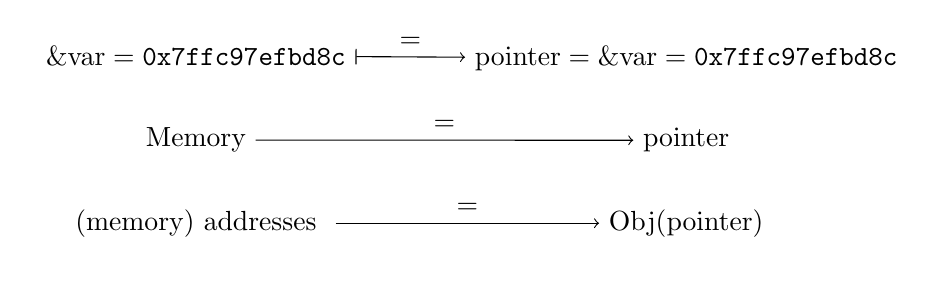
\begin{tikzpicture}
  \matrix (m) [matrix of math nodes, row sep=1.4em, column sep=4em, minimum width=1em]
  {
    \& \text{var} = \verb|0x7ffc97efbd8c| & \text{pointer} = \& \text{var} = \verb|0x7ffc97efbd8c| \\
     \text{Memory} & \text{pointer} \\
    \text{ (memory) addresses } & \text{Obj}(\text{pointer}) \\
  };
  \path[|->]
  (m-1-1) edge node [auto] {$=$} (m-1-2)
  ;
  \path[->]
  (m-2-1) edge node [auto] {$=$} (m-2-2)
  (m-3-1) edge node [auto] {$=$} (m-3-2)
  ;
  \end{tikzpicture}
\]

Referencing and deferencing operations on pointers to variables
\[
\begin{aligned}
  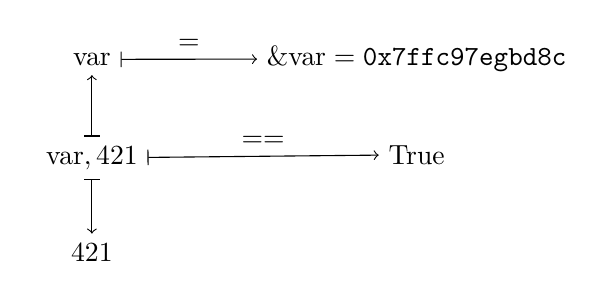
\begin{tikzpicture}
  \matrix (m) [matrix of math nodes, row sep=2em, column sep=4em, minimum width=1em]
  {
    \text{var} & \& \text{var} = \verb|0x7ffc97egbd8c| \\
    \text{var}, 421 & \text{True} \\
    421 &  \\
  };
  \path[|->]
  (m-1-1) edge node [auto] {$=$} (m-1-2)
  (m-2-1) edge node [auto] {$$} (m-1-1)
  edge node [auto] {$==$} (m-2-2)
  edge node [auto] {$$} (m-3-1)
  ;
  \end{tikzpicture}
    & 
  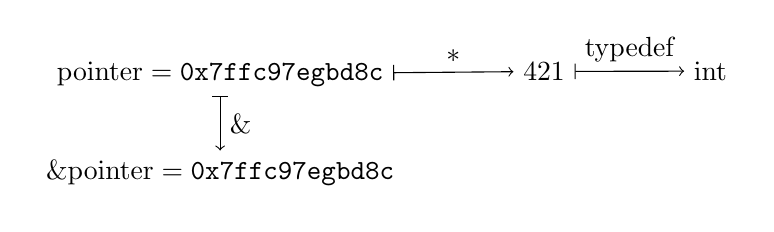
\begin{tikzpicture}
 \matrix (m) [matrix of math nodes, row sep=2em, column sep=4em, minimum width=1em]
  {
    \text{pointer} = \verb|0x7ffc97egbd8c| & 421 & \text{int} \\
    \& \text{pointer} = \verb|0x7ffc97egbd8c| & & \\ 
  };
  \path[|->]
  (m-1-1) edge node [auto] {$*$} (m-1-2)
  edge node [auto] {\&} (m-2-1)
  (m-1-2) edge node [auto] {\text{typedef}} (m-1-3)
;  
  \end{tikzpicture}   \\
    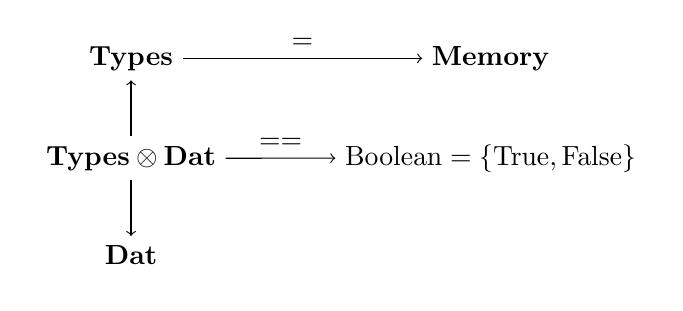
\begin{tikzpicture}
  \matrix (m) [matrix of math nodes, row sep=2em, column sep=4em, minimum width=1em]
  {
    \textbf{Types} &  \textbf{Memory}  \\
    \textbf{Types} \otimes \mathbf{\textbf{Dat}} & \text{Boolean} = \lbrace \text{True}, \text{False} \rbrace  \\
    \mathbf{\textbf{Dat}} &  \\
  };
  \path[->]
  (m-1-1) edge node [auto] {$=$} (m-1-2)
  (m-2-1) edge node [auto] {$$} (m-1-1)
  edge node [auto] {$==$} (m-2-2)
  edge node [auto] {$$} (m-3-1)
  ;
  \end{tikzpicture}
    & 
  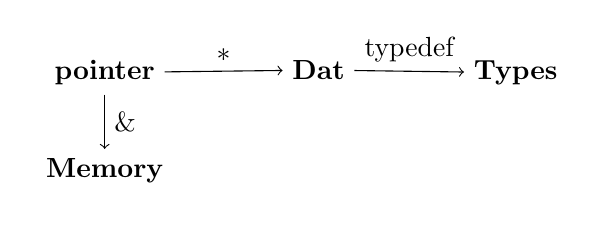
\begin{tikzpicture}
 \matrix (m) [matrix of math nodes, row sep=2em, column sep=4em, minimum width=1em]
  {
    \textbf{pointer}  & \mathbf{\textbf{Dat}} & \mathbf{\textbf{Types}} \\
    \mathbf{\textbf{Memory}} & & \\ 
  };
  \path[->]
  (m-1-1) edge node [auto] {$*$} (m-1-2)
  edge node [auto] {\&} (m-2-1)
  (m-1-2) edge node [auto] {\text{typedef}} (m-1-3)
;  
  \end{tikzpicture}   
  \end{aligned}
\]

\subsection{Numerical differentiation and interpolation (in C++)}

cf. Chapter 3 ``Numerical differentiation and interpolation'' of Hjorth-Jensen (2015) \cite{Hjor2015}.

This is how I understand it.

Consider the Taylor expansion for $f(x) \in C^{\infty}(\mathbb{R})$:
\[
f(x) = f(x_0)  + \sum_{j=1}^{\infty} \frac{ f^{(j)}(x_0)}{j!} h^j 
\]
For $x = x_0 \pm h$,
\[
\begin{gathered}
  f(x) = f(x_0 \pm h ) = f(x_0) + \sum_{j=1}^{\infty} \frac{ f^{(2j)}(x_0) }{(2j)!} h^{2j} \pm \sum_{j=1}^{\infty} \frac{ f^{(2j-1)}(x_0) }{(2j-1)!} h^{2j-1}
\end{gathered}
\]
Then
\[
\begin{gathered}
  f(x_0 + 2^kh) - f(x_0 - 2^kh) = 2\sum_{j=1}^{\infty} \frac{ f^{(2j-1)}}{(2j-1)!}(x_0) 2^{k(2j-1)} h^{2j-1} = \\
  = 2\left[ f^{(1)}(x_0) 2^k h + \sum_{j=2}^{\infty} \frac{ f^{(2j-1)}(x_0)}{ (2j-1)!} 2^{k(2j-1)} h^{2j-1} \right] =  \\
  = 2 \left[ f^{(1)}(x_0) 2^k h + \frac{ f^{(3)}(x_0)}{3!} 2^{k(3)} h^3 + \sum_{j=3}^{\infty} \frac{ f^{(2j-1)}(x_0) }{(2j-1)!} 2^{k(2j-1) } h^{2j-1} \right]
\end{gathered}
\]

So for $k=1$,
\[
f(x_0 + h ) - f(x_0 - h ) = 2 \left[ f^{(1)}(x_0)h + \sum_{j=1}^{\infty} \frac{ f^{(2j+1)}(x_0) }{ (2j+1)!} h^{2j+1} \right]
\]

Now
\[
\begin{gathered}
  f(x_0 + 2^kh) + f(x_0 - 2^kh) - 2f(x_0) = \\
  = 2 \sum_{j=1}^{\infty} \frac{ f^{(2j)}(x_0) }{(2j)!} 2^{2jk} h^{2j} = \\
  = 2 \left[ \frac{ f^{(2)}(x_0)}{2} 2^{2k} h^2 + \sum_{j=2}^{\infty} \frac{ f^{(2j)}(x_0) }{ (2j)!} 2^{2jk} h^{2j} \right] = \\
  = 2 \left[ \frac{ f^{(2)}(x_0) }{2} 2^{2k} h^2 + \frac{ f^{(4)}(x_0)}{4!} 2^{4k} h^4 + \sum_{j=3}^{\infty} \frac{ f^{(2j)}(x_0) }{ (2j)!} 2^{2jk} h^{2j} \right]
  \end{gathered}
\]
Thus for the case of $k=1$,
\[
f(x_0 + h )  + f(x_0 - h) - 2f(x_0) = f^{(2)}(x_0)h^2 + 2 \sum_{j=2}^{\infty} \frac{ f^{(2j)}(x_0)}{(2j)!} h^{2j}
\]
\[
\begin{aligned}
  & \frac{ f(x_0 +h) - f(x_0-h) }{ 2h} = f^{(1)}(x_0) + \sum_{j=1}^{\infty} \frac{ f^{(2j+1)}(x_0) }{(2j+1)!}h^{2j} \\ 
  & \frac{ f(x_0 + h) + f(x_0 - h) - 2f(x_0) }{h^2} = f^{(2)}(x_0) + 2\sum_{j=2}^{\infty} \frac{ f^{(2(j+1) ) }(x_0)}{(2(j+1))!} h^{2j}
  \end{aligned}
\]

A pattern now emerges on how to include more calculations at points $x_0, x_0 \pm 2^kh$ so to obtain better accuracy $O(h^l)$.  For instance,

Given 5 pts. $\lbrace x_0, x_0 \pm h, x_0 \pm 2h \rbrace$,
\[
\begin{gathered}
  f(x_0 + 2h) - f(x_0 -2h) = 2[ f^{(1)}(x_0) 2^1h + \frac{ f^{(3)}(x_0)}{3!} 2^3 h^3 + O(h^5) ] \\ 
  f(x_0+ h) - f(x_0 - h) = 2[ f^{(1)}(x_0) h + \frac{ f^{(3)}(x_0)}{3!} h^3 + O(h^5)] \\
  \Longrightarrow f'(x_0) = \frac{ f(x_0 - 2h) - 8f(x_0-h ) + 8f(x_0 + h) - f(x_0 + 2h) }{ 12h } + O(h^4)
\end{gathered}
\]

Hjorth-Jensen (2015) \cite{Hjor2015} argues, on pp. 46-47, that the additional evaluations are time consuming, to obtain further accuracy, so it's a balance.

To summarize, for $O(h^2)$ accuracy,
\[
\begin{aligned}
  & \frac{ f(x_0 + h) - f(x_0-h) }{2h} = f^{(1)}(x_0) + \sum_{j=1}^{\infty} \frac{ f^{(2j+1)}(x_0 )}{(2j+1)!} h^{2j} & \qquad \, O(h^2) \\ 
  & \frac{ f(x_0 + h) + f(x_0 -h) - 2f(x_0) }{h^2} = f^{(2)}(x_0) + 2\sum_{j=1}^{\infty} \frac{ f^{(2j+2)}(x_0) }{ (2j+2)!} h^{2j} & \qquad \, O(h^2)
  \end{aligned}
\]

\section{Interpolation}

cf. 3.2 Numerical Interpolation and Extrapolation of Hjorth-Jensen (2015) \cite{Hjor2015}

Given $N+1$ pts. $\begin{aligned} & \quad \\
  y_0 & = f(x_0) \\
  y_1 & = f(x_1) \\
  & \vdots \\
  y_N & = f(x_N) \end{aligned}$, $x_i$'s distinct (none of $x_i$ values equal)

We want a polynomial of degree $n$ s.t. $p(x)  \in \mathbb{R}[x]$

\[
p(x_i) = f(x_i) = y_i \qquad \, i = 0,1\dots N
\]

\[
p(x) = a_0 + a_1(x-x_0) + \dots + a_i \prod_{j=0}^{i-1}(x-x_j) + \dots + a_N(x-x_0) \dots (x-x_{N-1}) = a_0 + \sum_{i=1}^N a_i \prod_{j=0}^{i-1}(x-x_j)
\]
\[
\begin{aligned}
  & a_0 = f(x_0) \\ 
  & a_0 + a_1(x_1-x_0) = f(x_1) \\
  & \vdots \\
  & a_0 + \sum_{i=1}^k a_i \prod_{j=0}^{i-1} (x_k - x_j) = f(x_k)
  \end{aligned}
\]

Hjorth-Jensen (2015) \cite{Hjor2015} mentions this Lagrange interpolation formula (I haven't found a good proof for it).  
\begin{equation}
\boxed{ p_N(x) = \sum_{i=0}^N \prod_{k\neq i} \frac{ x-x_k}{x_i - x_k} y_i  }
\end{equation}

\section{Classes (C++)}

cf. \href{http://stackoverflow.com/questions/6377786/c-operator-overloading-in-expression}{C++ Operator Overloading in expression}

Take a look at this link: \href{http://stackoverflow.com/questions/6377786/c-operator-overloading-in-expression}{C++ Operator Overloading in expression}.  This point isn't emphasized enough, as in Hjorth-Jensen (2015) \cite{Hjor2015}.  This makes doing something like
\[
d = a*c + d/b
\]
work the way we expect.  Kudos to user \href{http://stackoverflow.com/users/252000/fredoverflow}{fredoverflow} for his answer:

``The expression \verb|(e_x*u_c)| is an rvalue, and references to non-const won't bind to rvalues.

Also, member functions should be marked \verb|const| as well.''  

\subsection{What are lvalues and rvalues in C and C++?}

\href{http://thbecker.net/articles/rvalue_references/section_01.html}{C++ Rvalue References Explained}

Original definition of \emph{lvalues} and \emph{rvalues} from \emph{C}: \\
\emph{lvalue} - expression $e$ that may appear on the left or on the right hand side of an assignment \\
\emph{rvalue} - expression that can only appear on right hand side of assignment $=$.

Examples:

\begin{lstlisting}
  int a = 42;
  int b = 43;

  // a and b are both l-values
  a = b; // ok
  b = a; // ok
  a = a * b; // ok

  // a * b is an rvalue:
  int c = a * b; // ok, rvalue on right hand side of assignment
  a * b = 42; // error, rvalue on left hand side of assignment
  
  \end{lstlisting}

In \emph{C++}, this is still useful as a first, intuitive approach, but \\
\emph{lvalue} - expression that refers to a memory location and allows us to take the address of that memory location via the $\&$ operator. \\
\emph{rvalue} - expression that's not a lvalue

So $\&$ reference \emph{functor} can't act on rvalue's.


\subsection{Functors (C++); C++ Functors; C++ class templates}
For categories $\mathbf{A}, \mathbf{B}$, consider trying to understand, wrap your mind around C++, especiall C++11/14 style functors.  The key \emph{insight} is \emph{composability}: use the mathematical property of \textbf{composition}.  
\begin{equation}
  \begin{gathered}
  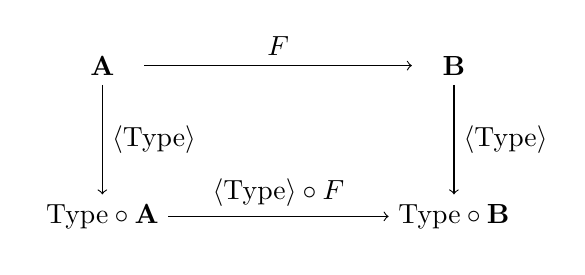
\begin{tikzpicture}
 \matrix (m) [matrix of math nodes, row sep=4em, column sep=8em, minimum width=3em]
  {
    \mathbf{A} & \mathbf{B}     \\
    \text{Type} \circ \mathbf{A} &    \text{Type} \circ \mathbf{B} \\ 
  };
  \path[->]
  (m-1-1) edge node [auto] {$F$} (m-1-2)
  edge node [auto] { $\langle \text{Type} \rangle$  } (m-2-1)
  (m-1-2) edge node [auto] { $\langle \text{Type} \rangle$  } (m-2-2)
  (m-2-1) edge node [auto] { $\langle \text{Type} \rangle \circ F $ } (m-2-2)
;  
  \end{tikzpicture}   
  \end{gathered}
  \end{equation}

This webpage from K Hong helped with understanding C++11/14 style functors: \href{http://www.bogotobogo.com/cplusplus/functors.php}{C++ Tutorial - Functors(Function Objects) - 2017}, cf. \url{http://www.bogotobogo.com/cplusplus/functors.php}

I implemented all of that in the webpage here: \href{https://github.com/ernestyalumni/CompPhys/blob/master/Cpp/Cpp14/functors.cpp}{github functors.cpp }, \verb|ernestyalumni/CompPhys/Cpp/Cpp14/functors.cpp|


I will try to write a dictionary between math, i.e. mathematical formulation, and the class templates, structs.

I looked at pp. 213 of Conlon, pp. 513 of Rotman, and looked up keywords ``functional.''

Consider the bilinear functional that results in a function, i.e. $\mathcal{C}^{\infty}(\mathbb{R})$.

\[
\mathbb{R} \times \mathbb{R} \to C^{\infty}(\mathbb{R})
\]
i.e.
\begin{equation}
\begin{aligned}
  & \mathbb{R} \times \mathbb{R} & \to \text{Hom}_{\mathbb{R}}(\mathbb{R}, \mathbb{R})   \\
  & (a,b) & \mapsto f(x) = ax + b
\end{aligned}
\end{equation}
with
\[
\text{Hom}_{\mathbb{R}}(\mathbb{R}, \mathbb{R}) \ni \lbrace \mathbb{R} \xrightarrow{f} \mathbb{R} \rbrace
\]
Compare this directly to \verb|class Line| in \verb|functor.cpp|.  Note that this is \emph{class object working as a functor}:

%\footnotesize{ 
\begin{lstlisting}
class Line {
	double a;			// slope
	double b; 			// y-intercept
	
	public:
		Line(double slope = 1, double yintercept = 1) : 
			a(slope), b(yintercept) { } 
		double operator()(double x){
			return a*x + b;
		}};
  \end{lstlisting}
%}
Now consider the use of C++ function object, but with non-type template, C++ templates:

\begin{equation}
\begin{aligned}
  & \mathbb{R} & \to & \text{Hom}_{\mathbb{R}}( \mathbb{R}, \mathbb{R} ) \\ 
  & x & \mapsto & f(y) = y + x 
  \end{aligned}
  \end{equation}
But suppose $y\in \mathbb{R}^d$, e.g. $y_i \in \mathbb{R}$, $i=0,1,\dots d-1$.

\begin{equation}
\begin{aligned}
  & \mathbb{R} & \to & \text{Hom}_{\mathbb{R}}( \mathbb{R}^d, \mathbb{R}^d ) \\ 
  & x & \mapsto & f(y) = y + x  \text{ or } (f(y))_i = y_i + x \qquad \, \forall \, i = 0, 1, \dots d-1
  \end{aligned}
  \end{equation}

So for the \emph{class template}, to generalize $\mathbb{R}$ to some choice of field $\mathbb{K}$, generalize $\mathbb{R}^d$ to R-module $R$.
\begin{equation}
\begin{aligned}
  & \mathbb{K} & \to & \text{Hom}_{\mathbb{K}}( \mathbb{K}, \mathbb{K} ) \\ 
  & x & \mapsto & (f(y))_i = y_i + x \qquad \, \forall \, i = 0, 1, \dots d-1
  \end{aligned}
  \end{equation}

And so the strategy is to generalize type by the class template (declaration), define the $\text{Hom}$ from $M$ to $M$ by defining the $\text{Hom}$ from $\mathbb{K}$ to $\mathbb{K}$ for each element of $M$.  

Compare this directly to the code for class Add in \verb|functor.cpp|:
%\footnotesize{
\begin{lstlisting}
  template <typename T>
class Add
{
	T x;
	
	public:
		Add(T xx) : x(xx) { } 
		void operator()(T& e) const { e += x; }
};
...


std::for_each(v2.begin(), v2.end(), Add<int>(10));

	std::for_each(v2.begin(), v2.end(), Add<int>(*v2.begin()) );
        
\end{lstlisting}
%}
Notice how the construction of the $\text{Hom}$ needs an input.  


\section{Numerical Integration}

\subsubsection{Trapezoid rule (or trapezoidal rule)}

See \href{https://github.com/ernestyalumni/CompPhys/blob/master/Cpp/Integrate.ipynb}{Integrate.ipynb}.

From there, consider integration on $[a,b]$, considering $h := \frac{b-a}{N}$, and $N+1$ (grid) points, $\lbrace a, a+h, a+2h, \dots , a+ jh, \dots , a+Nh = b\rbrace_{j=0 \dots N }$.

Then $\frac{N}{2}$ pts. are our ``$x_0$''; $x_0$'s $= \lbrace a +h , a+3h, \dots , a+(2j-1)h, \dots , a+ \left( \frac{2 N}{2} - 1 \right)h \rbrace_{j=1 \dots \frac{N}{2} }$.

Notice how we really need to care about if $N$ is even or not.  If $N$ is not even, then we'd have to deal with the integration at the integration limits and choosing what to do.  

Then
\[
\begin{gathered}
  \int_a^b f(x) dx = \sum_{j=1}^{N/2} \int_{a + (2j-1)h-h}^{a+(2j-1)h+h} f(x)dx = \sum_{j=1}^{N/2} \frac{h}{2} ( 2f(a+(2j-1)h ) + f(a+2(j-1)h) + f(a+2jh) ) = \\
   = h(f(a)/2 + f(a+h) + \dots + f(b-h) + \frac{f(b)}{2} ) = h \left( \frac{f(a)}{2} + \sum_{j=1}^{N-1} f(a+jh) + \frac{f(b)}{2} \right)
  \end{gathered}
\]

\subsubsection{Midpoint method or rectangle method}.

Let $h := \frac{b-a}{N}$ be the step size.  The grid is as follows:
\[
\lbrace a , a +h , \dots , a + jh , \dots , a+Nh = b\rbrace_{j=0\dots N}
\]
The desired midpoint values are at the following $N$ points:
\[
\lbrace a + \frac{h}{2} , a + \frac{3}{2} h , \dots , a+\frac{(2j-1 ) h }{2} , \dots , a + \left( N - \frac{1}{2} \right) h \rbrace_{j=1 \dots N}
\]
and so
\begin{equation}
  \int_a^b f(x) dx \approx \sum_{j=1}^N f(x_j) h = \sum_{j=1}^N f\left( a + \frac{(2j-1) h}{2} \right)h 
\end{equation}


\subsubsection{Simpson rule}

The idea is to take the next ``order'' in the Lagrange interpolation formula, the second-order polynomial, and then we can rederive Simpson's rule.  The algebra is worked out in \href{https://github.com/ernestyalumni/CompPhys/blob/master/Cpp/Integrate.ipynb}{Integrate.ipynb}.

From there, then we can obtain Simpson's rule,
\[
\begin{gathered}
  \int_a^b f(x)dx = \sum_{j=1}^{N/2} \int_{a + 2(j-1)h }^{a+2jh} f(x) dx = \sum_{j=1}^{N/2} \frac{h}{3} ( 4 f(a+(2j-1)h ) + f(a+2(j-1)h) + f(a+2jh) ) = \\
  = \frac{h}{3} \left[ f(a) + f(b) + \sum_{j=1}^{N/2} 4f(a+(2j-1) h) + 2\sum_{j=1}^{N/2-1} f(a+2jh) \right]
\end{gathered}
\]

\subsection{Gaussian Quadrature}

cf. Hjorth-Jensen (2015) \cite{Hjor2015}, Section 5.3 Gaussian Quadrature, Chapter 5 Numerical Integration


\section{Runge-Kutta methods (RK) }

cf. Hjorth-Jensen (2015) \cite{Hjor2015}, Section 8.4 \emph{More on finite difference methods, Runge-Kutta methods} and \emph{wikipedia}, ``Runge-Kutta methods,'' \url{https://en.wikipedia.org/wiki/Runge\%E2\%80\%93Kutta_methods}

While Runge-Kutta methods are useful initially for ordinary differential equations, remember that under certain (very general, in fact, for smooth manifolds even) conditions, vector fields admit integral lines and there you simply solve an system of linear ODEs.  


\section{Partial Differential Equations}

\subsubsection{Explicit Scheme}
cf. Hjorth-Jensen (2015) \cite{Hjor2015}, Section 10.2.1 Explicit Scheme

Consider
\begin{equation}
\begin{gathered}
  \begin{gathered}
    u = u(t,x) \in C^{\infty}(M) = C^{\infty}(\mathbb{R}\times N)  
  \end{gathered} \\
      \Delta u = \frac{ \partial u}{ \partial t}(t,x)
  \end{gathered}
  \end{equation}
with initial conditions
\[
  \begin{gathered}
    u(0,x)=g(x) \qquad \, \forall \, 0 < x < L_x \text{ or } x \in \Omega \subset N \, \text{(in general)}
    \end{gathered}
  \]
  e.g. $L_x=1$ \\

  and boundary conditions
  \[
\begin{aligned}
  & u(t,0) = a(t) & t \geq 0 \\ 
  & u(t,L) = b(t) & t \geq 0 
\end{aligned}
  \]

  Consider the act of discretization as a transformation or a functor:
  \begin{equation}
\begin{gathered}
  \frac{ \partial u}{ \partial t} = \frac{ u(t+\Delta t,x) - u(t,x) }{ \Delta t} + O(\Delta t) \xrightarrow{ \text{ discretize } } \frac{ u(t_j + \Delta t, x_i) - u(t_j,x_i) }{ \Delta t } \\
  \frac{ \partial^2 u}{ \partial (x^i)^2 } \approx \frac{ u(t,x + \Delta x) - 2 u(t,x) + u(t, x-\Delta x) }{ (\Delta x)^2 }  \xrightarrow{ \text{ discretize } } \frac{ u(t_j  , x_i+\Delta x) - 2 u(t_j,x_i) + u(t_j,x_i-\Delta x) }{ ( \Delta x)^2 } 
\end{gathered}
  \end{equation}

  \begin{equation}
\Longrightarrow u(t_j + \Delta t, x_i) = \frac{ \Delta t}{ (\Delta x)^2 } u(t_j,x_i + \Delta x) + \left( 1 - \frac{ 2 \Delta t}{ (\Delta x)^2 } \right) u (t_j,x_i) + \frac{ \Delta t}{ (\Delta x)^2 } u(t_j,x_i - \Delta x)
  \end{equation}

  Discretize the initial conditions:
  \begin{equation}
u(0,x) = g(x) \xrightarrow{ \text{ discretize } } u(0,x_i) = g(x_i)
\end{equation}

and so, for the first step,
\begin{equation}
u(\Delta t, x_i) = \frac{ \Delta t}{ (\Delta x)^2 } g(x_i + \Delta x) + \left( 1 - \frac{ 2 \Delta t}{ (\Delta x)^2 } \right) g(x_i) + \frac{ \Delta t}{ (\Delta x)^2 } g(x_i - \Delta x)
\end{equation}
It would appear to be instructive to show what discretize is doing, as a commutative diagram:
\begin{equation}
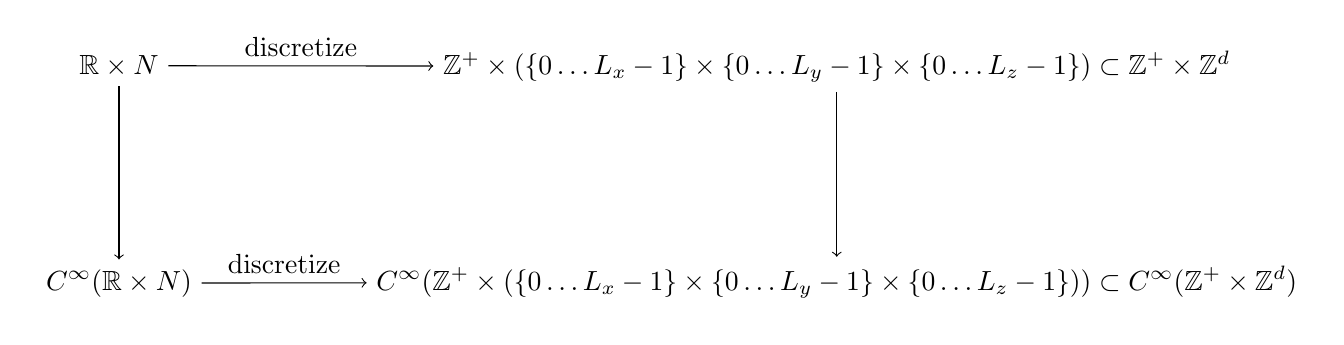
\begin{tikzpicture}
 \matrix (m) [matrix of math nodes, row sep=6em, column sep=6em, minimum width=1em]
  {
    \mathbb{R} \times N           &  \mathbb{Z}^+ \times ( \lbrace 0 \dots L_x-1 \rbrace \times \lbrace 0 \dots L_y-1 \rbrace \times \lbrace 0 \dots L_z -1 \rbrace) \subset \mathbb{Z}^+ \times \mathbb{Z}^d   \\
    C^{\infty}(\mathbb{R}\times N)  & C^{\infty}( \mathbb{Z}^+ \times ( \lbrace 0 \dots L_x-1 \rbrace \times \lbrace 0 \dots L_y -1 \rbrace \times \lbrace 0 \dots L_z -1 \rbrace ) ) \subset C^{\infty}(\mathbb{Z}^+ \times \mathbb{Z}^d)  \\ 
  };
  \path[->]
  (m-1-1) edge node [auto] { \text{discretize}} (m-1-2)
  edge node [auto] {} (m-2-1)
  (m-2-1) edge node [auto] { \text{ discretize } } (m-2-2)
  (m-1-2) edge node [auto] { } (m-2-2) 
;  
  \end{tikzpicture}   
  \end{equation}
  Then there's this so-called ``sparse'' (I think this means that there are a lot more zeros as values for the entries in a matrix than there are nonzero values), tridiagonal (diagonal and next to the diagonal, diagonals) matrices representation of the time-evolution transformation/operator.  I'll call this transformation over to this matrix representation, this functor, \emph{matricer}.

\begin{equation}
  \begin{gathered}
    C^{\infty}(\mathbb{Z}^+ \times ( \lbrace 0 \dots L_x-1 \rbrace \times \lbrace 0 \dots L_y -1 \rbrace \times \lbrace 0 \dots L_z -1 \rbrace ) ) \xrightarrow{ \text{ matricer } } \mathbb{Z}^+ \times \mathbb{R}^{ L_x L_y L_z} = \mathbb{Z}^+ \times \text{Mat}_{\mathbb{R}}(L_x,L_y,L_z)
    \end{gathered}
\end{equation}

  For the boundary conditions,
\[
\begin{gathered}
  \begin{aligned}
    & u(t,0) = a(t) & \qquad \, t \geq 0 \\ 
    & u(t,L) = b(t) & \qquad \, t \geq 0 
    \end{aligned} \xrightarrow{ \text{ discretize } }   \begin{aligned}
    & u(t,0) = a(t)    \\ 
    & u(t,x_{L_x-1}) = b(t)  
    \end{aligned}
\end{gathered}
\]

  For 1-dim. case, $V_j \in \text{Mat}_{\mathbb{R}}(L_x)$ (vector or ``column'' matrix)
\[
  V_j = \left[ \begin{matrix} u(t_j,x_2) \\
      u(t_j,x_3) \\
      \vdots \\
      u(t_j,x_{L_x-3}) \end{matrix} \right]
\]
  and so the ``time-evolution'' operator/transformation is
\begin{equation}
  \begin{gathered}
    \widehat{A} \in \text{Mat}_{\mathbb{R}}(L_x-4,L_x-4) = \text{End}(\mathbb{R}^{L_x-4}, \mathbb{R}^{L_x-4}) \\
    \widehat{A} = \left[ \begin{matrix}
         \frac{ \Delta t}{ (\Delta x)^2 } & 1 -  2 \frac{ \Delta t}{ (\Delta x)^2 } &  \frac{ \Delta t}{ (\Delta x)^2 } & 0 & 0 & \dots & 0  \\ 
         0 &  \frac{ \Delta t}{ (\Delta x)^2 } & 1 - 2  \frac{ \Delta t}{ (\Delta x)^2 } &  \frac{ \Delta t}{ (\Delta x)^2 } & 0 & \dots & 0 \\
         &  &  & \ddots  &   &   & \\
      0   & 0  & \dots  & 0        &  \frac{ \Delta t}{ (\Delta x)^2 } & 1 - 2  \frac{ \Delta t}{ (\Delta x)^2 } &  \frac{ \Delta t}{ (\Delta x)^2 } 
        \end{matrix} \right]
  \end{gathered}
\end{equation}  

Note that in the specialized 1-dim. case where $a(t) = b(t)=0$ (boundary conditions for both ends is of value $0$), then we can, in this specialized case, define the matrix $\widehat{A}$ to be
\begin{equation}
  \begin{gathered}
    \widehat{A} \in \text{Mat}_{\mathbb{R}}(L_x-2,L_x-2) = \text{End}(\mathbb{R}^{L_x-2}, \mathbb{R}^{L_x-2}) \\
    \widehat{A} = \left[ \begin{matrix}
        1 - 2  \frac{ \Delta t}{ (\Delta x)^2 } &  \frac{ \Delta t}{ (\Delta x)^2 } & 0 & 0 & \dots  &  0 & 0 \\
         \frac{ \Delta t}{ (\Delta x)^2 } & 1 -  2 \frac{ \Delta t}{ (\Delta x)^2 } &  \frac{ \Delta t}{ (\Delta x)^2 } & 0 & 0 & \dots & 0  \\ 
         0 &  \frac{ \Delta t}{ (\Delta x)^2 } & 1 - 2  \frac{ \Delta t}{ (\Delta x)^2 } &  \frac{ \Delta t}{ (\Delta x)^2 } & 0 & \dots & 0 \\
         &  &  & \ddots  &   &   & \\
         0   & 0  & \dots  & 0        &  \frac{ \Delta t}{ (\Delta x)^2 } & 1 - 2  \frac{ \Delta t}{ (\Delta x)^2 } &  \frac{ \Delta t}{ (\Delta x)^2 }  \\
         0 & 0 & 0 & \dots & 0 &  \frac{ \Delta t}{ (\Delta x)^2 } & 1 - 2  \frac{ \Delta t}{ (\Delta x)^2 } 
        \end{matrix} \right]
  \end{gathered}
\end{equation}  

e.g.
\[
g(x) = \sin{ \left( \frac{ \pi }{ l_x} x \right) }
\]
with an analytic solution of
\[
u(t,x) = \sin{ \left( \frac{\pi}{l_x}x \right) } \exp{ \left( - \left( \frac{\pi}{l_x}\right)^2 t \right) }
\]

It was bizarre to me that in Hjorth-Jensen (2015) \cite{Hjor2015}, Section 10.2.1 Explicit Scheme, on pp. 307, Hjorth-Jensen went through a lengthy and thorough explanation of this ``matricer'' operation, i.e. doing the time-evolution with a matrix on a vector of values at grid points, and yet in the pseudo-code, essentially, there is no trace of that matrix!  It's essentially a local ``stencil'' operation.  What the heck?

I present the ``matrix form'' code in my github repository: \href{https://github.com/ernestyalumni/CompPhys/blob/master/Cpp/progs/ch10pde/diffusion1dexplicit.cpp}{`diffusion1dexplicit.cpp`}.  To be explicit, the code follows the previous writeup, with its notation, essentially one-to-one.  

\subsubsection{Implicit scheme}
cf. Hjorth-Jensen (2015) \cite{Hjor2015}, Section 10.2.2 Implicit Scheme

Consider
\begin{equation}
\begin{aligned}
  & \text{ backwards formula : }       & \frac{ \partial u }{ \partial t}(t,x) \approx \frac{ u(t_j,x_i) - u(t_j-\Delta t, x_i) }{ \Delta t} \text{ or even } \\
  & \text{ midpoint approximations : } &  \frac{ \partial u }{ \partial t}(t,x) \approx \frac{ u(t_j + \Delta t,x_i) - u(t_j-\Delta t, x_i) }{ 2 \Delta t}
\end{aligned}
\end{equation}

Consider the same spatial discretization as before for the Laplacian:
\[
\frac{ \partial^2 u}{ \partial (x^i)^2 } \approx \frac{ u(t,x + \Delta x) - 2 u(t,x) + u(t, x-\Delta x) }{ (\Delta x)^2 }  \xrightarrow{ \text{ discretize } } \frac{ u(t_j  , x_i+\Delta x) - 2 u(t_j,x_i) + u(t_j,x_i-\Delta x) }{ ( \Delta x)^2 } 
\]
and so for the backwards formula case, 
\begin{equation}
  \begin{gathered}
 \frac{ u(t_j,x_i) - u(t_j-\Delta t, x_i) }{ \Delta t}   =  \frac{ u(t_j  , x_i+\Delta x) - 2 u(t_j,x_i) + u(t_j,x_i-\Delta x) }{ ( \Delta x)^2 }  \\
 u(t_j - \Delta t, x_i) = -\frac{ \Delta t}{ (\Delta x)^2 } u(t_j,x_i + \Delta x) + \left( 1 + \frac{ 2 \Delta t}{ (\Delta x)^2 } \right) u (t_j,x_i) - \frac{ \Delta t}{ (\Delta x)^2 } u(t_j,x_i - \Delta x)
    \end{gathered}
 \end{equation}
resulting in the backwards time-evolution matrix $\widehat{A}$ (keeping in mind the special boundary condition of $0$ value for $u$ at both ends, for the sake of a simplified discussion):
\begin{equation}
  \begin{gathered}
    \widehat{A} \in \text{Mat}_{\mathbb{R}}(L_x-2,L_x-2) = \text{End}(\mathbb{R}^{L_x-2}, \mathbb{R}^{L_x-2}) \\
    \widehat{A} = \left[ \begin{matrix}
        1 + 2  \frac{ \Delta t}{ (\Delta x)^2 } &  -\frac{ \Delta t}{ (\Delta x)^2 } & 0 & 0 & \dots  &  0  \\
         -\frac{ \Delta t}{ (\Delta x)^2 } & 1 +  2 \frac{ \Delta t}{ (\Delta x)^2 } &  -\frac{ \Delta t}{ (\Delta x)^2 } & 0 &  \dots & 0  \\ 
                 &  &  & \ddots  &   &   & \\
         0   & 0  & \dots  &   -\frac{ \Delta t}{ (\Delta x)^2 } & 1 + 2  \frac{ \Delta t}{ (\Delta x)^2 } & - \frac{ \Delta t}{ (\Delta x)^2 }  \\
         0 & 0 & 0 & \dots &  - \frac{ \Delta t}{ (\Delta x)^2 } & 1 + 2  \frac{ \Delta t}{ (\Delta x)^2 } 
        \end{matrix} \right]
  \end{gathered}
\end{equation}  
\[
\widehat{A}u^j = u^{j-1}
\]
and so
\[
\widehat{A}^{-1}u^{j-1} = u^j
\]

\subsection{Crank-Nicolson method}

Hjorth-Jensen (2015) \cite{Hjor2015}, Section 10.2.3 Crank Nicholson scheme has a write up about the Crank-Nicolson method, but the derivation is unclear (and sloppy, in that after the Taylor expansions, he says that the terms magically add up to the desired result, and the ``approximation'' notation is vacuous in that nothing new was conveyed).  Rather, look at \href{http://people.sc.fsu.edu/~jpeterson/5-CrankNicolson.pdf}{Crank Nicolson Scheme for the Heat Equation} for a clearer derivation, that drives home the point of looking at the time between time steps.

Consider the following Taylor expansions about $t^{1/2} := t + \frac{ \Delta t}{2}$.

\[
\begin{aligned}
  & u(t+\Delta t,x) = u(t + \frac{ \Delta t}{2} + \frac{ \Delta t}{2} ,x ) \equiv u(t^{1/2} + \frac{ \Delta t}{2} ,x ) = u(t^{1/2},x) + \frac{ \Delta t}{2} \frac{ \partial u}{\partial t}(t^{1/2},x) + \frac{1}{2} \left( \frac{ \Delta t}{2} \right)^2 \frac{ \partial^2 u}{\partial t^2}(t^{1/2},x) + O((\Delta t)^3) \\ 
  & u(t,x) = u(t + \frac{ \Delta t}{2} - \frac{ \Delta t}{2} ,x ) \equiv u(t^{1/2} - \frac{ \Delta t}{2} ,x ) = u(t^{1/2},x) - \frac{ \Delta t}{2} \frac{ \partial u}{\partial t}(t^{1/2},x) + \frac{1}{2} \left( \frac{ \Delta t}{2} \right)^2 \frac{ \partial^2 u}{\partial t^2}(t^{1/2},x) + O((\Delta t)^3)    \\
  & u(t+\Delta t,x) - u(t,x) = \Delta t \frac{ \partial u}{ \partial t}(t^{1/2},x) + O((\Delta t)^3) 
\end{aligned}
\]
\[
\Longrightarrow \frac{ \partial u}{ \partial t}(t^{1/2},x) = \frac{ u(t+\Delta t,x) - u(t,x) }{\Delta t}
\]
with $O((\Delta t)^2)$ order of accuracy.

To approximate
\[
\frac{ \partial^2 u}{ \partial x^2}(t+ \frac{ \Delta t}{2}, x) \equiv \frac{ \partial^2 u}{ \partial x^2}(t^{1/2},x) 
\]
use average of second, centered differences for $\frac{ \partial^2 u}{ \partial x^2}(t+\Delta t,x) $ and $\frac{ \partial^2 u}{ \partial x^2}(t,x)$.

\[
\begin{gathered}
\frac{ \partial^2 u}{ \partial x^2 }(t+\frac{\Delta t}{2},x) \approx \frac{1}{2} \left[ \frac{ u(t+ \Delta t, x+\Delta x) - 2u(t+\Delta t,x) + u(t+\Delta t,x-\Delta x) }{ (\Delta x)^2 } + \frac{ u(t,x+\Delta x) - 2u(t,x) + u(t,x-\Delta x) }{ (\Delta x)^2 } \right]
  \end{gathered}
\]
Then for
\[
\begin{gathered}
  \frac{ \partial u }{ \partial t}(t^{1/2},x) = C_0 \Delta u(t^{1/2},x) \xrightarrow{ discretize } \\ 
  u(t+\Delta t,x)-u(t,x) = \\
   = \frac{1}{2} C_0 \frac{\Delta t}{(\Delta x)^2 }(u(t+\Delta t, x+\Delta x) - 2u(t+\delta t, x) + u(t+\Delta t,x-\Delta x) ) + \frac{1}{2} C_0 \frac{ \Delta t}{ (\Delta x)^2 }u(t,x+\Delta x) + \frac{ -\Delta t}{(\Delta x)^2 }C_0 u(t,x) + \frac{1}{2} \frac{ \Delta t}{ (\Delta x)^2 }C_0u(t,x-\Delta x)
  \end{gathered}
  \]

  Let
\[
  \alpha := \frac{ \Delta t}{ (\Delta x)^2 }
  \]
Then
\begin{equation}
  \frac{-1}{2} \alpha u(t+\Delta t, x+\Delta x) + (1+\alpha) u(t+\Delta t,x) - \frac{\alpha}{2} u(t+\Delta t, x-\Delta x) = \frac{ \alpha}{2}u(t,x+\Delta x) + (1-\alpha)u(t,x) + \frac{\alpha}{2}u(t,x-\Delta x)
\end{equation}
  
In general
\begin{equation}
\begin{gathered}
  \frac{-\alpha}{2} C_0 u(t+\Delta t,x+\Delta x) + (1 + C_0 \alpha)u(t+\Delta t,x) - \frac{ C_0 \alpha}{2} u(t+\Delta t, x-\Delta x) = \\
  = \frac{ C_0 \alpha}{2} u(t,x+\Delta x) + (1- C_0 \alpha)u(t,x) + \frac{C_0\alpha}{2}u(t,x-\Delta x)
  \end{gathered}
  \end{equation}

This scheme necessitates a matrix representation.  In matrix form,
\begin{equation}
  \begin{gathered}
    \left[ \begin{matrix}
        1 + C_0 \alpha & - \frac{ \alpha C_0}{2} & 0 & \dots & 0 & 0 & \dots & 0 \\
        \frac{ -C_0\alpha}{2} & 1 + C_0 \alpha & \frac{ -\alpha C_0 }{2} & 0 & 0 & \dots & 0 \\
        0 & \frac{ -C_0 \alpha}{2} & 1 +C_0\alpha & \frac{ -C_0 \alpha}{2} & 0 & \dots & 0 \\
         &                         &              & \ddots &                   &      &   \\
        0 & 0 & \dots & 0 & \frac{-\alpha}{2} & 1 + C_0 \alpha & \frac{-\alpha}{2} \\
        0 & 0 & \dots & 0 & 0                 & \frac{ -\alpha}{2} & 1 + C_0 \alpha \end{matrix} \right] u_i^{t+\Delta t} = \\
    = \left[ \begin{matrix}
        1 - C_0 \alpha & \frac{C_0 \alpha }{2} & 0 & 0 & 0 & \dots & 0 \\
        \frac{C_0 \alpha}{2} & 1 - C_0 \alpha & \frac{C_0 \alpha}{2} & 0 & 0 & \dots 0 \\
        0 & \frac{C_0 \alpha}{2} & 1 - C_0\alpha & \frac{C_0 \alpha}{2} & 0 & \dots & 0 \\
        &                       &               & \ddots             &    &      & \\
        0 & 0 & 0                        & \dots & \frac{C_0 \alpha}{2} & 1 - C_0 \alpha & \frac{C_0 \alpha}{2} \\
        0 & 0 & 0 &                \dots &  0  & \frac{C_0 \alpha}{2} & 1 - C_0 \alpha \end{matrix} \right]  u_i^t  \\
    \Longrightarrow \widehat{B} u_i^{t+ \Delta t } = \widehat{A} u_i^{t} \text{ or } \\
    u_i^{t+\Delta t} = \widehat{B}^{-1}\widehat{A}u_i^t
\end{gathered}
\end{equation}

\subsection{Jacobi method, SOR method, for the Laplace and Poisson equation}

\href{http://www.physics.buffalo.edu/phy410-505/2011/topic3/app1/index.html}{3.1 Poisson's Equation and Relaxation Methods} of 410-505 Physics had a good, online, clear explanation of Jacobi method and improvements, namely the Successive Over Relaxation (SOR) method, applied to Laplace and Poisson equation, with clearly labelled diagrams: \url{http://www.physics.buffalo.edu/phy410-505/2011/topic3/app1/index.html}





\section{Call by reference - Call by Value, Call by reference (in C and in C++)}

cf. pp. 58, 2.10 Pointers Ch. 2 Scientific Programming in C, Fitzpatrick \cite{Fitz}
\verb|printfact3.c|, \href{https://github.com/ernestyalumni/CompPhys/blob/master/CFitz/printfact3.c}{printfact3.c}

pass pointer, pass by reference, call by pointer, call by reference 

In C: 
\begin{itemize}
  \item  \emph{function prototype} - 
\[
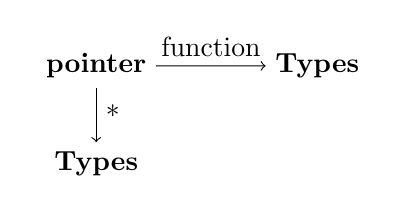
\begin{tikzpicture}
 \matrix (m) [matrix of math nodes, row sep=2em, column sep=4em, minimum width=1em]
  {
    \textbf{pointer}  &  \textbf{Types} \\
    \textbf{Types}  & \\ 
  };
  \path[->]
  (m-1-1) edge node [auto] { \text{function}} (m-1-2)
  edge node [auto] {*} (m-2-1)
;  
  \end{tikzpicture}   
\qquad \qquad \, \,
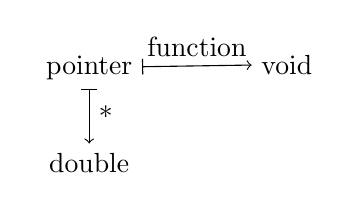
\begin{tikzpicture}
 \matrix (m) [matrix of math nodes, row sep=2em, column sep=4em, minimum width=1em]
  {
    \text{pointer}  &  \text{void} \\
    \text{double}  & \\ 
  };
  \path[|->]
  (m-1-1) edge node [auto] { \text{function}} (m-1-2)
  edge node [auto] {*} (m-2-1)
;  
  \end{tikzpicture}   
\]
$\Longrightarrow$ 
\begin{lstlisting}
void factorial(double *)
  \end{lstlisting}
where for factorial, it's just your choice of name for \emph{function}.  

\item \emph{function definition} - 
  \[
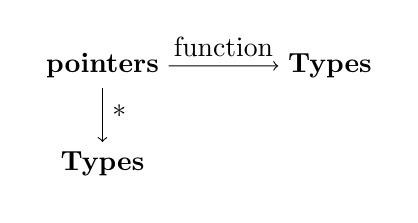
\begin{tikzpicture}
 \matrix (m) [matrix of math nodes, row sep=2em, column sep=4em, minimum width=1em]
  {
    \textbf{pointers}  &  \textbf{Types} \\
    \textbf{Types}  & \\ 
  };
  \path[->]
  (m-1-1) edge node [auto] { \text{function}} (m-1-2)
  edge node [auto] {*} (m-2-1)
;  
\end{tikzpicture}   \qquad  \,
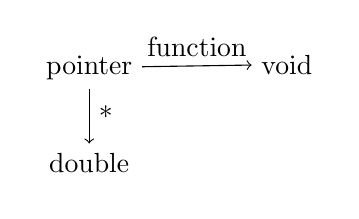
\begin{tikzpicture}
 \matrix (m) [matrix of math nodes, row sep=2em, column sep=4em, minimum width=1em]
  {
    \text{pointer}  &  \text{void} \\
    \text{double}  & \\ 
  };
  \path[->]
  (m-1-1) edge node [auto] { \text{function}} (m-1-2)
  edge node [auto] {*} (m-2-1)
;  
  \end{tikzpicture}   \qquad \, 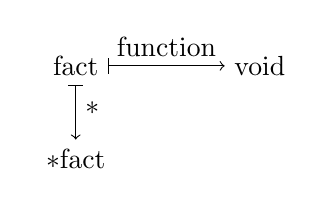
\begin{tikzpicture}
 \matrix (m) [matrix of math nodes, row sep=2em, column sep=4em, minimum width=1em]
  {
    \text{fact}  &  \text{void} \\
    *\text{fact}  & \\ 
  };
  \path[|->]
  (m-1-1) edge node [auto] { \text{function}} (m-1-2)
  edge node [auto] {*} (m-2-1)
;  
  \end{tikzpicture}   
\]
  $\Longrightarrow$
\begin{lstlisting}
  void function(double *fact) { ... }
\end{lstlisting}

\emph{Inside} the function definition,
\[
  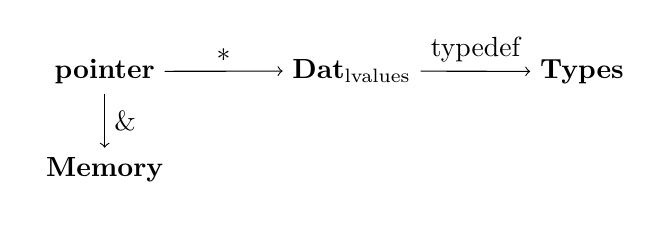
\begin{tikzpicture}
 \matrix (m) [matrix of math nodes, row sep=2em, column sep=4em, minimum width=1em]
  {
    \textbf{pointer}  & \textbf{Dat}_{\text{lvalues}} & \textbf{Types} \\
    \textbf{Memory} & & \\ 
  };
  \path[->]
  (m-1-1) edge node [auto] {$*$} (m-1-2)
  edge node [auto] {\&} (m-2-1)
  (m-1-2) edge node [auto] {\text{typedef}} (m-1-3)
;  
  \end{tikzpicture} \qquad \qquad \,   
  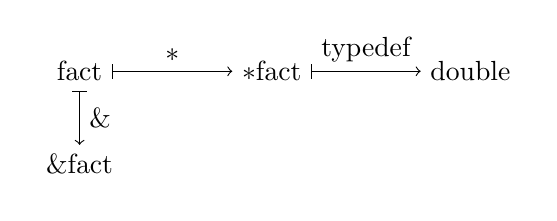
\begin{tikzpicture}
 \matrix (m) [matrix of math nodes, row sep=2em, column sep=4em, minimum width=1em]
  {
    \text{fact}  & *\text{fact}  & \text{double} \\
    \& \text{fact} & & \\ 
  };
  \path[|->]
  (m-1-1) edge node [auto] {$*$} (m-1-2)
  edge node [auto] {\&} (m-2-1)
  (m-1-2) edge node [auto] {\text{typedef}} (m-1-3)
;  
  \end{tikzpicture}   
  \]
  and so, for instance, in the function definition, you can do things like this:
  \begin{lstlisting}
    *fact = 1
    *fact *= (double) n 
    \end{lstlisting}
and so notice that from \verb|*fact = 1|, \verb|*fact| is a lvalue.  
  \begin{itemize}
  \item \emph{ function procedure }
\[
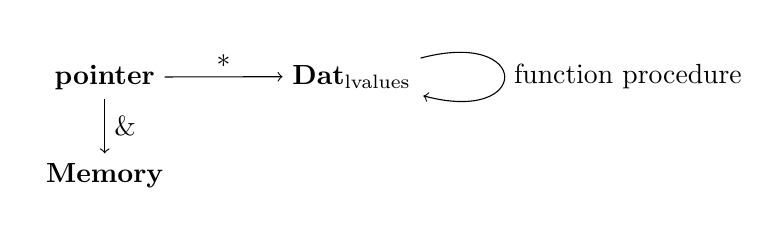
\begin{tikzpicture}
 \matrix (m) [matrix of math nodes, row sep=2em, column sep=4em, minimum width=1em]
  {
    \textbf{pointer}  & \textbf{Dat}_{\text{lvalues}}     \\
     \textbf{Memory} &  \\ 
  };
  \path[->]
  (m-1-1) edge node [auto] {$*$} (m-1-2)
  edge node [auto] {\&} (m-2-1)
  (m-1-2) [loop right] edge node [right] {\text{function procedure}} (m-1-2)
;  
  \end{tikzpicture}    \qquad \qquad \, 
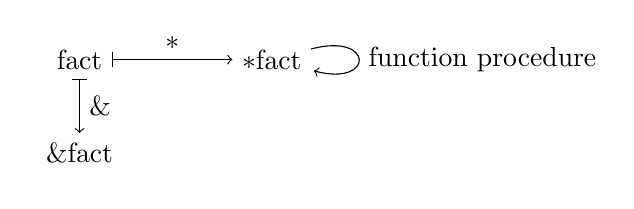
\begin{tikzpicture}
 \matrix (m) [matrix of math nodes, row sep=2em, column sep=4em, minimum width=1em]
  {
    \text{fact}  & * \text{fact}     \\
    \& \text{fact} &  \\ 
  };
  \path[|->]
  (m-1-1) edge node [auto] {$*$} (m-1-2)
  edge node [auto] {\&} (m-2-1)
  (m-1-2) [loop right] edge node [right] {\text{function procedure}} (m-1-2)
;  
    \end{tikzpicture}
\]
$\Longrightarrow $
\begin{lstlisting}
  *fact *= (double) n 
\end{lstlisting}
    \end{itemize}

\item ``Using'' the function, function ``instantiation'', ``calling'' the function, i.e. ``running'' the function
  \[
  \begin{aligned} 
& 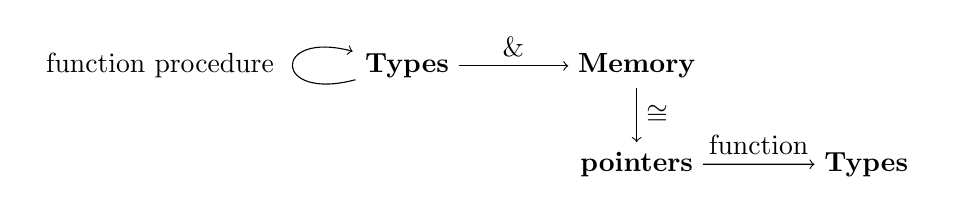
\begin{tikzpicture}
 \matrix (m) [matrix of math nodes, row sep=2em, column sep=4em, minimum width=1em]
  {
    \textbf{Types}  &  \textbf{Memory} &     \\
                    & \textbf{pointers} & \textbf{Types}  \\ 
  };
  \path[->]
  (m-1-1) edge node [auto] {$\&$} (m-1-2)
  (m-1-2) edge node [auto] {$\cong$ } (m-2-2)
  (m-2-2)  edge node [auto] {\text{function}} (m-2-3)
  (m-1-1) [loop left] edge node [left] { \text{ function procedure } } (m-1-1)
  ;  
\end{tikzpicture} \qquad \, \\
    & 
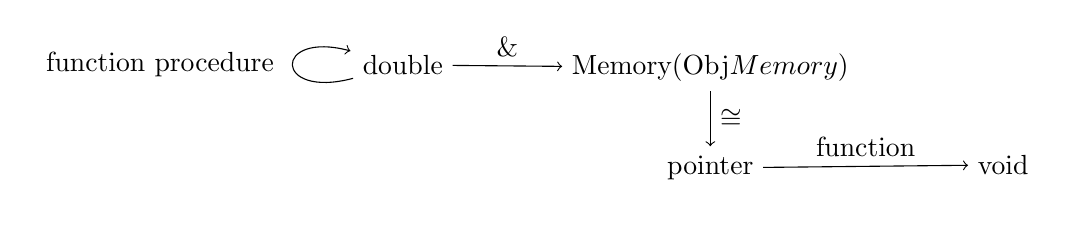
\begin{tikzpicture}
 \matrix (m) [matrix of math nodes, row sep=2em, column sep=4em, minimum width=1em]
  {
    \text{double}  &  \text{Memory} (\text{Obj}{Memory}) &     \\
                    & \text{pointer} & \text{void}  \\ 
  };
  \path[->]
  (m-1-1) edge node [auto] {$\&$} (m-1-2)
  (m-1-2) edge node [auto] {$\cong$ } (m-2-2)
  (m-2-2)  edge node [auto] {\text{function}} (m-2-3)
  (m-1-1) [loop left] edge node [left] { \text{ function procedure } } (m-1-1)
  ;  
\end{tikzpicture} \qquad \, \\
&
 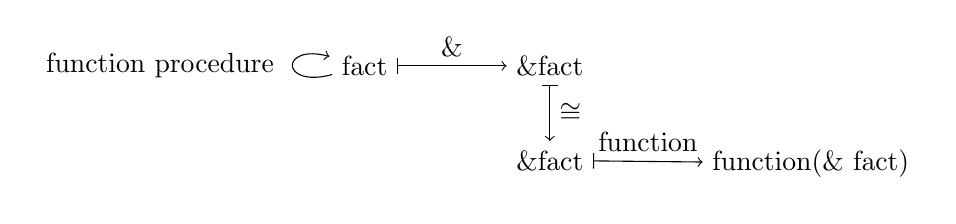
\begin{tikzpicture}
 \matrix (m) [matrix of math nodes, row sep=2em, column sep=4em, minimum width=1em]
  {
    \text{fact}  &  \& \text{fact}  &     \\
                    & \& \text{fact} & \text{function}(\& \text{ fact})  \\ 
  };
  \path[|->]
  (m-1-1) edge node [auto] {$\&$} (m-1-2)
  (m-1-2) edge node [auto] {$\cong$ } (m-2-2)
  (m-2-2)  edge node [auto] {\text{function}} (m-2-3)
  (m-1-1) [loop left] edge node [left] { \text{ function procedure } } (m-1-1)
  ;  
\end{tikzpicture}
\end{aligned}
    \]
    where, again simply note the notation, that we're using \emph{function} and \emph{factorial}, \emph{fact} for \emph{nameofpointer}, interchangeably: see \href{https://github.com/ernestyalumni/CompPhys/blob/master/CFitz/printfact3.c}{printfact3.c} for the example I'm referring to.

    
\end{itemize}

Again, \emph{in C}, consider \emph{a pointer to a function} passed to another function as an argument.  Take a look at \href{https://github.com/ernestyalumni/CompPhys/blob/master/CFitz/passfunction.c}{passfunction.c} simultaneously.

\begin{itemize}
\item  \emph{function prototype} -
\[
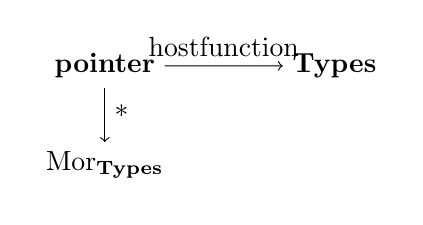
\begin{tikzpicture}
 \matrix (m) [matrix of math nodes, row sep=2em, column sep=4em, minimum width=1em]
  {
    \textbf{pointer}  &  \textbf{Types} \\
    \text{Mor}_{\textbf{Types}}  & \\ 
  };
  \path[->]
  (m-1-1) edge node [auto] { \text{hostfunction}} (m-1-2)
  edge node [auto] {*} (m-2-1)
;  
  \end{tikzpicture}   
\qquad \qquad \, \,
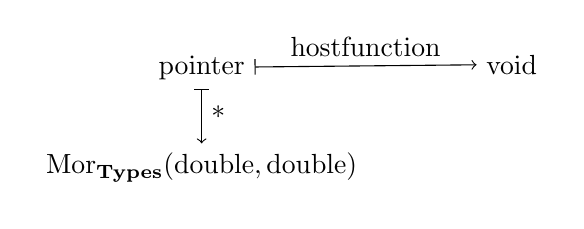
\begin{tikzpicture}
 \matrix (m) [matrix of math nodes, row sep=2em, column sep=4em, minimum width=1em]
  {
    \text{pointer}  &  \text{void} \\
    \text{Mor}_{\textbf{Types}}(\text{double},\text{double})  & \\ 
  };
  \path[|->]
  (m-1-1) edge node [auto] { \text{hostfunction}} (m-1-2)
  edge node [auto] {*} (m-2-1)
;  
  \end{tikzpicture}   
\]
$\Longrightarrow$
\begin{lstlisting}
  void hostfunction(double (*)(double))
\end{lstlisting}
We could further generalize this syntax, simply for syntax and notation sake, as such:
\[
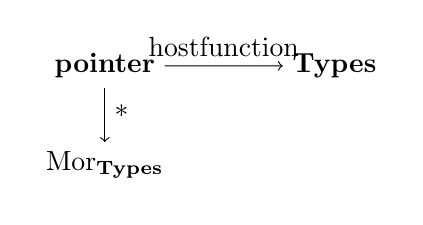
\begin{tikzpicture}
 \matrix (m) [matrix of math nodes, row sep=2em, column sep=4em, minimum width=1em]
  {
    \textbf{pointer}  &  \textbf{Types} \\
    \text{Mor}_{\textbf{Types}}  & \\ 
  };
  \path[->]
  (m-1-1) edge node [auto] { \text{hostfunction}} (m-1-2)
  edge node [auto] {*} (m-2-1)
;  
  \end{tikzpicture}   
\qquad \qquad \, \,
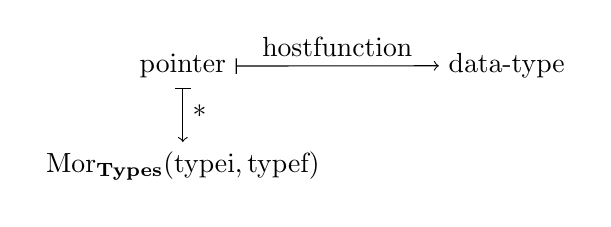
\begin{tikzpicture}
 \matrix (m) [matrix of math nodes, row sep=2em, column sep=4em, minimum width=1em]
  {
    \text{pointer}  &  \text{data-type} \\
    \text{Mor}_{\textbf{Types}}(\text{typei},\text{typef})  & \\ 
  };
  \path[|->]
  (m-1-1) edge node [auto] { \text{hostfunction}} (m-1-2)
  edge node [auto] {*} (m-2-1)
;  
  \end{tikzpicture}   
\]
$\Longrightarrow$
\begin{lstlisting}
  data-type hostfunction(typef (*)(typei))
\end{lstlisting}

For practice, consider more than 1 argument in our function, and the other argument, for practice, is a pointer, we're ``passing by reference.''

\[
\begin{aligned}
  & 
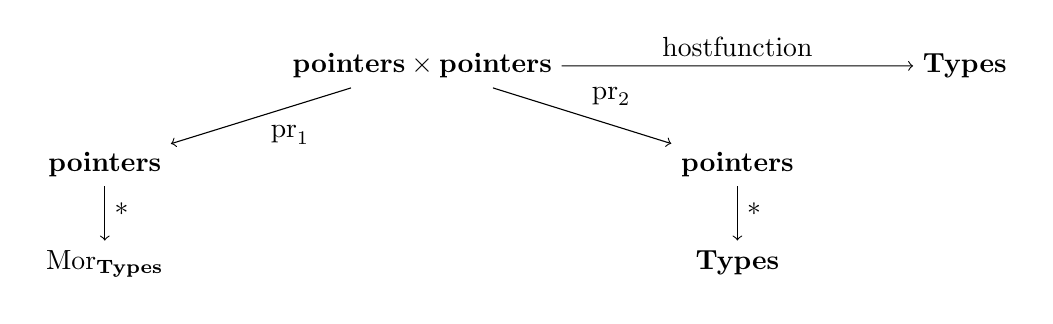
\begin{tikzpicture}
 \matrix (m) [matrix of math nodes, row sep=2em, column sep=4em, minimum width=1em]
  {
    & \textbf{pointers} \times \textbf{pointers}  &   & \textbf{Types} \\
    \textbf{pointers} &  & \textbf{pointers} & \\      
    \text{Mor}_{\textbf{Types}}  &  & \textbf{Types} &  \\ 
  };
  \path[->]
  (m-1-2) edge node [auto] { \text{hostfunction}} (m-1-4)
  (m-1-2) edge node [auto] { $\text{pr}_1$ } (m-2-1)
  edge node [auto] { $\text{pr}_2$ } (m-2-3)
  (m-2-1) edge node [auto] {*} (m-3-1)
  (m-2-3) edge node [auto] {*} (m-3-3)
  ;  
  \end{tikzpicture}   
\qquad \qquad \, \, \\
&
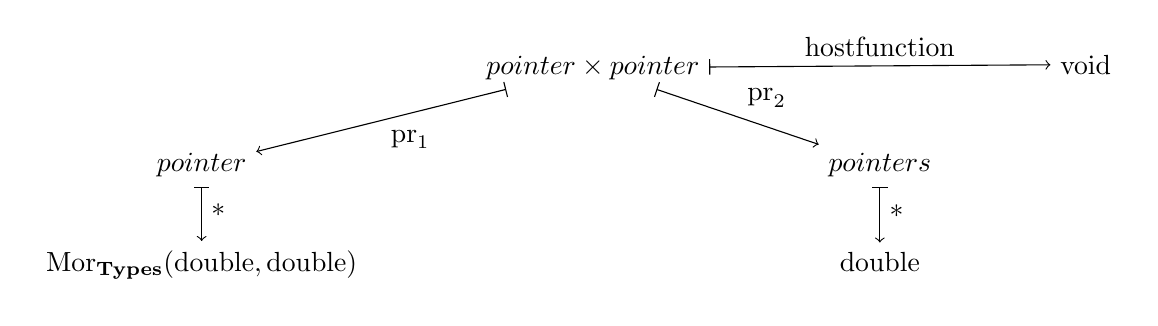
\begin{tikzpicture}
 \matrix (m) [matrix of math nodes, row sep=2em, column sep=4em, minimum width=1em]
  {
    & pointer \times pointer  &   & \text{void} \\
    pointer &  & pointers & \\      
    \text{Mor}_{\textbf{Types}}(\text{double},\text{double})  &  & \text{double} &  \\ 
  };
  \path[|->]
  (m-1-2) edge node [auto] { \text{hostfunction}} (m-1-4)
  (m-1-2) edge node [auto] { $\text{pr}_1$ } (m-2-1)
  edge node [auto] { $\text{pr}_2$ } (m-2-3)
  (m-2-1) edge node [auto] {*} (m-3-1)
  (m-2-3) edge node [auto] {*} (m-3-3)
  ;  
  \end{tikzpicture}   
\end{aligned}
\]
$\Longrightarrow$
\begin{lstlisting}
void hostfunction( double (*)(double), double *)
\end{lstlisting}
\item \emph{function definition}

  \[
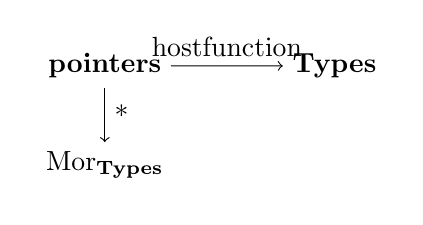
\begin{tikzpicture}
 \matrix (m) [matrix of math nodes, row sep=2em, column sep=4em, minimum width=1em]
  {
    \textbf{pointers}  &  \textbf{Types} \\
    \text{Mor}_{\textbf{Types}}  & \\ 
  };
  \path[->]
  (m-1-1) edge node [auto] { \text{hostfunction}} (m-1-2)
  edge node [auto] {*} (m-2-1)
;  
\end{tikzpicture}   \qquad  \,
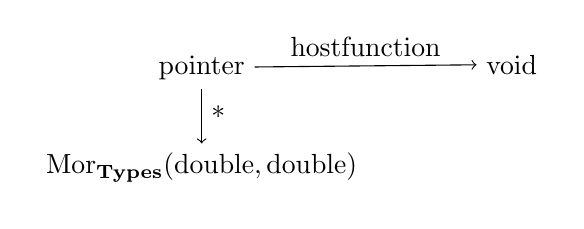
\begin{tikzpicture}
 \matrix (m) [matrix of math nodes, row sep=2em, column sep=4em, minimum width=1em]
  {
    \text{pointer}  &  \text{void} \\
    \text{Mor}_{\textbf{Types}}(\text{double},\text{double})  & \\ 
  };
  \path[->]
  (m-1-1) edge node [auto] { \text{hostfunction}} (m-1-2)
  edge node [auto] {*} (m-2-1)
;  
  \end{tikzpicture}   \qquad \, 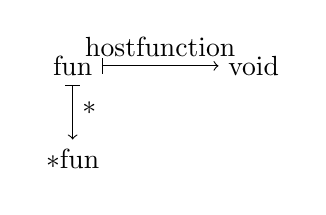
\begin{tikzpicture}
 \matrix (m) [matrix of math nodes, row sep=2em, column sep=4em, minimum width=1em]
  {
    \text{fun}  &  \text{void} \\
    *\text{fun}  & \\ 
  };
  \path[|->]
  (m-1-1) edge node [auto] { \text{hostfunction}} (m-1-2)
  edge node [auto] {*} (m-2-1)
;  
  \end{tikzpicture}   
\]
  $\Longrightarrow$
\begin{lstlisting}
  void hostfunction(double (*fun)(double)) { ... }
\end{lstlisting}

\item \emph{Inside} the function definition,
\[
\begin{aligned}
  & 

\begin{tikzpicture}
 \matrix (m) [matrix of math nodes, row sep=2em, column sep=4em, minimum width=1em]
  {
    \textbf{Types}  &  \textbf{Types} & \textbf{Types} \\
  };
  \path[->]
  (m-1-1) edge node [auto] { $*\text{fun}$} (m-1-2)
  (m-1-2) edge node [auto] {$=$} (m-1-3)
;  
\end{tikzpicture} \quad \, \\
& 
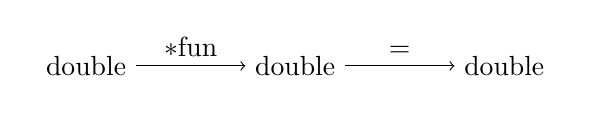
\begin{tikzpicture}
 \matrix (m) [matrix of math nodes, row sep=2em, column sep=4em, minimum width=1em]
  {
    \text{double}  &  \text{double} & \text{double} \\
  };
  \path[->]
  (m-1-1) edge node [auto] { $*\text{fun}$} (m-1-2)
  (m-1-2) edge node [auto] {$=$} (m-1-3)
;  
\end{tikzpicture}   \quad \, \\
&
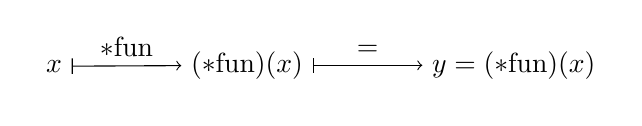
\begin{tikzpicture}
 \matrix (m) [matrix of math nodes, row sep=2em, column sep=4em, minimum width=1em]
  {
    x  &  (*\text{fun})(x) & y = (*\text{fun})(x) \\
  };
  \path[|->]
  (m-1-1) edge node [auto] { $*\text{fun}$} (m-1-2)
  (m-1-2) edge node [auto] {$=$} (m-1-3)
;  
  \end{tikzpicture}   
\end{aligned}
\]
$\Longrightarrow $
\begin{lstlisting}
y = (*fun)(x)
  \end{lstlisting}
\item ``Using'' the function - the \emph{actual} syntax for ``passing'' a function into a function is interesting (peculiar?): you only need the \emph{name} of the function.

  Let's quickly recall how a function is prototyped, ``declared'' (or, i.e., defined), and used:
  \begin{itemize}
  \item \emph{function prototype} -
    \[
\begin{aligned}
  &
  \begin{tikzpicture}
 \matrix (m) [matrix of math nodes, row sep=2em, column sep=4em, minimum width=1em]
  {
    \textbf{Types} & \textbf{Types} \\ 
  };
  \path[->]
  (m-1-1) edge node [auto] { $\text{fun}1$} (m-1-2)
;  
  \end{tikzpicture}   
  \qquad \, \\
  &
  \begin{tikzpicture}
 \matrix (m) [matrix of math nodes, row sep=2em, column sep=4em, minimum width=1em]
  {
    \text{double} & \text{double} \\ 
  };
  \path[->]
  (m-1-1) edge node [auto] { $\text{fun}1$} (m-1-2)
;  
  \end{tikzpicture}   
\end{aligned}
    \]
    $\Longrightarrow $
    \begin{lstlisting}
      double fun1(double)
    \end{lstlisting}
  \item \emph{ function definition } -
    \[
\begin{aligned}
  &
  \begin{tikzpicture}
 \matrix (m) [matrix of math nodes, row sep=2em, column sep=4em, minimum width=1em]
  {
    \textbf{Types} & \textbf{Types} \\ 
  };
  \path[->]
  (m-1-1) edge node [auto] { $\text{fun}1$} (m-1-2)
;  
  \end{tikzpicture}   
  \qquad \, \\
  &
  \begin{tikzpicture}
 \matrix (m) [matrix of math nodes, row sep=2em, column sep=4em, minimum width=1em]
  {
    \text{double} & \text{double} \\ 
  };
  \path[->]
  (m-1-1) edge node [auto] { $\text{fun}1$} (m-1-2)
;  
  \end{tikzpicture}
  \qquad \, \\
  &
    \begin{tikzpicture}
 \matrix (m) [matrix of math nodes, row sep=2em, column sep=4em, minimum width=1em]
  {
    z & 3.0 z*z - z (= 3z^2 - z) \\ 
  };
  \path[|->]
  (m-1-1) edge node [auto] { $\text{fun}1$} (m-1-2)
;  
  \end{tikzpicture}   
\end{aligned}
    \]
    $\Longrightarrow $
    \begin{lstlisting}
      double fun1(double z) { ... }
    \end{lstlisting}
    \item Using function - \verb| fun1(z) |

        \end{itemize}
  and so
  \[
\text{fun}1 \in \text{Mor}_{\textbf{Types}}(\text{double},\text{double})
\]

And so again, it's interesting in terms of syntax that all you need is the \emph{name} of the function to pass into the arguments of the ``host function'' when using the host function:
\[
\begin{gathered}
    \begin{tikzpicture}
 \matrix (m) [matrix of math nodes, row sep=2em, column sep=4em, minimum width=1em]
  {
  \text{Mor}_{\textbf{Types}} & \textbf{Types} \\ 
  };
  \path[->]
  (m-1-1) edge node [auto] { $\text{hostfunction}$} (m-1-2)
;  
  \end{tikzpicture}   
    \\
        \begin{tikzpicture}
 \matrix (m) [matrix of math nodes, row sep=2em, column sep=4em, minimum width=1em]
  {
  \text{Mor}_{\textbf{Types}}(\text{double},\text{double}) & \text{void} \\
  };
  \path[|->]
  (m-1-1) edge node [auto] { $\text{hostfunction}$} (m-1-2)
;  
        \end{tikzpicture}   \\
                \begin{tikzpicture}
 \matrix (m) [matrix of math nodes, row sep=2em, column sep=4em, minimum width=1em]
  {
  \text{fun}1 & \text{hostfunction}(\text{fun}1) \\
  };
  \path[|->]
  (m-1-1) edge node [auto] { $\text{hostfunction}$} (m-1-2)
;  
  \end{tikzpicture}   
  \end{gathered}
\]
$\Longrightarrow$
\begin{lstlisting}
hostfunction(fun1)
  \end{lstlisting}

\end{itemize}

\subsubsection{C++ extensions, or how C++ pass by reference (pass a pointer to argument) vs. C}

Recall how C passes by reference, and look at Fitzpatrick \cite{Fitz}, pp. 83-84 for the \verb|square| function:

\begin{itemize}
  \item  \emph{function prototype} - 
\[
\begin{tikzpicture}
 \matrix (m) [matrix of math nodes, row sep=2em, column sep=4em, minimum width=1em]
  {
    \textbf{pointer}  &  \textbf{Types} \\
    \textbf{Types}  & \\ 
  };
  \path[->]
  (m-1-1) edge node [auto] { \text{square}} (m-1-2)
  edge node [auto] {*} (m-2-1)
;  
  \end{tikzpicture}   
\qquad \qquad \, \,
\begin{tikzpicture}
 \matrix (m) [matrix of math nodes, row sep=2em, column sep=4em, minimum width=1em]
  {
    \text{pointer}  &  \text{void} \\
    \text{double}  & \\ 
  };
  \path[|->]
  (m-1-1) edge node [auto] { \text{square}} (m-1-2)
  edge node [auto] {*} (m-2-1)
;  
  \end{tikzpicture}   
\]
$\Longrightarrow$ 
\begin{lstlisting}
void square(double *)
  \end{lstlisting}

\item \emph{function definition} - 
  \[
\begin{tikzpicture}
 \matrix (m) [matrix of math nodes, row sep=2em, column sep=4em, minimum width=1em]
  {
    \textbf{pointers}  &  \textbf{Types} \\
    \textbf{Types}  & \\ 
  };
  \path[->]
  (m-1-1) edge node [auto] { \text{square}} (m-1-2)
  edge node [auto] {*} (m-2-1)
;  
\end{tikzpicture}   \qquad  \,
\begin{tikzpicture}
 \matrix (m) [matrix of math nodes, row sep=2em, column sep=4em, minimum width=1em]
  {
    \text{pointer}  &  \text{void} \\
    \text{double}  & \\ 
  };
  \path[->]
  (m-1-1) edge node [auto] { \text{function}} (m-1-2)
  edge node [auto] {*} (m-2-1)
;  
  \end{tikzpicture}   \qquad \, \begin{tikzpicture}
 \matrix (m) [matrix of math nodes, row sep=2em, column sep=4em, minimum width=1em]
  {
    y  &  \text{void} \\
    *y  & \\ 
  };
  \path[|->]
  (m-1-1) edge node [auto] { \text{square}} (m-1-2)
  edge node [auto] {*} (m-2-1)
;  
  \end{tikzpicture}   
\]
  $\Longrightarrow$
\begin{lstlisting}
  void square(double *y) { ... }
\end{lstlisting}

\emph{Inside} the function definition,
\[
  \begin{tikzpicture}
 \matrix (m) [matrix of math nodes, row sep=2em, column sep=4em, minimum width=1em]
  {
    \textbf{pointer}  & \textbf{Dat}_{\text{lvalues}} & \textbf{Types} \\
  };
  \path[->]
  (m-1-1) edge node [auto] {$*$} (m-1-2)
  (m-1-2) edge node [auto] {\text{typedef}} (m-1-3)
;  
  \end{tikzpicture} \qquad \qquad \,   
  \begin{tikzpicture}
 \matrix (m) [matrix of math nodes, row sep=2em, column sep=4em, minimum width=1em]
  {
    y  & *y  & \text{double} \\
  };
  \path[|->]
  (m-1-1) edge node [auto] {$*$} (m-1-2)
  (m-1-2) edge node [auto] {\text{typedef}} (m-1-3)
;  
  \end{tikzpicture}   
  \]
  and so, for instance, in the function definition, you can do things like this:
  \begin{lstlisting}
    *y = x*x
    \end{lstlisting}

\item ``Using'' the function, function ``instantiation'', ``calling'' the function, i.e. ``running'' the function
  \[
  \begin{aligned} 
& \begin{tikzpicture}
 \matrix (m) [matrix of math nodes, row sep=2em, column sep=4em, minimum width=1em]
  {
    \textbf{Types}  &  \textbf{Memory} &     \\
                    & \textbf{pointers} & \textbf{Types}  \\ 
  };
  \path[->]
  (m-1-1) edge node [auto] {$\&$} (m-1-2)
  (m-1-2) edge node [auto] {$\cong$ } (m-2-2)
  (m-2-2)  edge node [auto] {\text{square}} (m-2-3)
  (m-1-1) [loop left] edge node [left] { \text{ function procedure } } (m-1-1)
  ;  
\end{tikzpicture} \qquad \, \\
    & 
\begin{tikzpicture}
 \matrix (m) [matrix of math nodes, row sep=2em, column sep=4em, minimum width=1em]
  {
    \text{double}  &  \text{Memory} (\text{Obj}{Memory}) &     \\
                    & \text{pointer} & \text{void}  \\ 
  };
  \path[->]
  (m-1-1) edge node [auto] {$\&$} (m-1-2)
  (m-1-2) edge node [auto] {$\cong$ } (m-2-2)
  (m-2-2)  edge node [auto] {\text{square}} (m-2-3)
  (m-1-1) [loop left] edge node [left] { \text{ function procedure } } (m-1-1)
  ;  
\end{tikzpicture} \qquad \, \\
&
 \begin{tikzpicture}
 \matrix (m) [matrix of math nodes, row sep=2em, column sep=4em, minimum width=1em]
  {
    \text{res}  &  \& \text{res}  &     \\
                    & \& \text{res} & \text{square}(\& \text{res})  \\ 
  };
  \path[|->]
  (m-1-1) edge node [auto] {$\&$} (m-1-2)
  (m-1-2) edge node [auto] {$\cong$ } (m-2-2)
  (m-2-2)  edge node [auto] {\text{square}} (m-2-3)
  (m-1-1) [loop left] edge node [left] { \text{ function procedure } } (m-1-1)
  ;  
\end{tikzpicture}
\end{aligned}
    \]
    
\end{itemize}

\subsubsection{C++ syntax for dealing with passing pointers (and arrays) into functions}

However, in \emph{C++}, a lot of the dereferencing $*$ and referencing $\&$ is not explicitly said so in the syntax.  In this syntax, passing by reference is indicated by prepending the $\&$ ampersand to the variable name, in function declaration (prototype and definition).  We don't have to explicitly deference the argument in the function (it's done behind the scene) and syntax-wise (it seems), we only have to refer to the argument by regular local name.

Indeed, the syntax appears ``shortcutted'' greatly:
\begin{itemize}
  \item  \emph{function prototype} - 
\[
\begin{tikzpicture}
 \matrix (m) [matrix of math nodes, row sep=2em, column sep=4em, minimum width=1em]
  {
    \textbf{pointer} \times \textbf{Types}  &  \textbf{Types} \\
  };
  \path[->]
  (m-1-1) edge node [auto] { \text{function}} (m-1-2)
;  
  \end{tikzpicture}   
\qquad \qquad \, \,
\begin{tikzpicture}
 \matrix (m) [matrix of math nodes, row sep=2em, column sep=4em, minimum width=1em]
  {
    \text{pointer}, \text{double}  &  \text{void} \\
  };
  \path[|->]
  (m-1-1) edge node [auto] { \text{function}} (m-1-2)
;  
  \end{tikzpicture}   
\]
$\Longrightarrow$ 
\begin{lstlisting}
void function(double &)
  \end{lstlisting}

\item \emph{function definition} - 
  \[
\begin{tikzpicture}
 \matrix (m) [matrix of math nodes, row sep=2em, column sep=4em, minimum width=1em]
  {
    \textbf{pointers}\times \textbf{Types}  &  \textbf{Types} \\
  };
  \path[->]
  (m-1-1) edge node [auto] { \text{square}} (m-1-2)
;  
\end{tikzpicture}   \qquad  \,
\begin{tikzpicture}
 \matrix (m) [matrix of math nodes, row sep=2em, column sep=4em, minimum width=1em]
  {
    \text{pointer},\text{double}  &  \text{void} \\
  };
  \path[->]
  (m-1-1) edge node [auto] { \text{function}} (m-1-2)
;  
  \end{tikzpicture}   \qquad \, \begin{tikzpicture}
 \matrix (m) [matrix of math nodes, row sep=2em, column sep=4em, minimum width=1em]
  {
   \&, y  &  \text{function}(\text{double} \; \& y) \\
  };
  \path[|->]
  (m-1-1) edge node [auto] { \text{function}} (m-1-2)
;  
  \end{tikzpicture}   
\]
  $\Longrightarrow$
\begin{lstlisting}
  void function(double &y) { ... }
\end{lstlisting}

\emph{Inside} the function definition,
\[
  \begin{tikzpicture}
 \matrix (m) [matrix of math nodes, row sep=2em, column sep=4em, minimum width=1em]
  {
    \text{double}   & \text{double} \\
  };
  \path[->]
  (m-1-1) edge node [auto] {$\text{End}(\text{double},\text{double})$} (m-1-2)
;  
  \end{tikzpicture} \qquad \qquad \,   
  \begin{tikzpicture}
 \matrix (m) [matrix of math nodes, row sep=2em, column sep=4em, minimum width=1em]
  {
    y  & y = x*x \\
  };
  \path[|->]
  (m-1-1) edge node [auto] {$\text{End}(\text{double},\text{double})$} (m-1-2)
;  
  \end{tikzpicture}   
  \]
  and so, for instance, in the function definition, you can do things like this:
  \begin{lstlisting}
    y = x*x
    \end{lstlisting}
with no deferencing needed.  
\item ``Using'' the function, function ``instantiation'', ``calling'' the function, i.e. ``running'' the function
  \[
  \begin{aligned} 
& \begin{tikzpicture}
 \matrix (m) [matrix of math nodes, row sep=2em, column sep=4em, minimum width=1em]
  {
    \textbf{Types}  &  \textbf{Types}      \\
  };
  \path[->]
  (m-1-1) edge node [auto] {$\text{function}$} (m-1-2)
  ;  
\end{tikzpicture} \qquad \,      
\begin{tikzpicture}
 \matrix (m) [matrix of math nodes, row sep=2em, column sep=4em, minimum width=1em]
  {
    \text{double}  &  \text{void}  \\
  };
  \path[->]
  (m-1-1) edge node [auto] {$\text{function}$} (m-1-2)
  ;  
\end{tikzpicture} \qquad \, 
 \begin{tikzpicture}
 \matrix (m) [matrix of math nodes, row sep=2em, column sep=4em, minimum width=1em]
  {
    \text{res}  &   \text{function}(\text{res})       \\
                     };
  \path[|->]
  (m-1-1) edge node [auto] {$\text{function}$} (m-1-2)
  ;  
\end{tikzpicture}
\end{aligned}
    \]
    
\end{itemize}

\subsubsection{C++ note on arrays}

For dealing with arrays, Stroustrup (2013) \cite{Stro2013}, on pp. 12 of Chapter 1 The Basics, Section 1.8 Pointers, Arrays, and References, does the following:

\begin{itemize}
\item \emph{array declaration} -
  \begin{lstlisting}
    type a[n]; // type[n]; array of n type's
  \end{lstlisting}
\item ``Using'' arrays in function prototypes, i.e. passing into arguments of functions for \emph{function prototypes}
  \begin{lstlisting}
    data-type function( type * arrayname)
    \end{lstlisting}
\item ``Using'' arrays when ``using'' functions, i.e. passing into arguments when a function is ``called'' or ``executed''
  \begin{lstlisting}
    function( arrayname )
  \end{lstlisting}
  \end{itemize}


Fitzpatrick \cite{Fitz} mentions using \verb|inline| for short functions, no more than 3 lines long, because of memory cost of calling a function.  




\subsubsection{Need a CUDA, C, C$++$, IDE?  Try Eclipse!}

This website has a clear, lucid, and pedagogical tutorial for using Eclipse: \href{https://www.fayewilliams.com/2011/06/28/creating-your-first-c-program-in-eclipse/}{Creating Your First C++ Program in Eclipse}.  But it looks like I had to pay.  Other than the well-written tips on the webpage, I looked up stackexchange for my Eclipse questions (I had difficulty with the Eclipse documentation).  

Others, like myself, had questions on how to use an IDE like Eclipse when learning CUDA, and ``building'' (is that the same as compiling?) and running only single files.  

My workflow: I have a separate, in my file directory, folder with my github repository clone that's local.

I start a New Project, CUDA Project, in Eclipse.  I type up my single file (I right click on the \verb|src| folder and add a `Source File`).  I build it (with the Hammer, Hammer looking icon; yes there are a lot of new icons near the top) and it runs.  I can then run it again with the Play, triangle, icon.

I found that if I have more than 1 (2 or more) file in the \verb|src| folder, that requires the \verb|main| function, it won't build right.

So once a file builds and it's good, I, in Terminal, \verb|cp| the file into my local github repository.  Note that from there, I could use the \verb|nvcc| compiler to build, from there, if I wanted to.

Now with my file saved (for example, \verb|helloworldkernel.cu|), then I can delete it, without fear, from my, say, \verb|cuda-workplace|, from the right side, ``C/C$++$ Projects'' window in Eclipse.   

\section{On CUDA By Example}
Take a look at 3.2.2 A Kernel Call, a Hello World in CUDA C, with a simple kernel, on pp. 23 of Sanders and Kandrot (2010) \cite{SK2010} and on github, [helloworldkernel.cu](https://github.com/ernestyalumni/CompPhys/blob/master/CUDA-By-Example/helloworldkernel.cu).  Let's work out the functor interpretation for practice.

\begin{itemize}
\item \emph{function definition} - \[
  \begin{gathered}
    \textbf{Types} \xrightarrow{ \text{ kernel } } \textbf{Types } \\ 
    \text{void} \xrightarrow{ \text{kernel } } \text{ void }
  \end{gathered}
  \]
  where \verb|kernel| $\in $ \verb|__global__| \\
  $\Longrightarrow $
  \begin{lstlisting}
    __global__ void kernel(void) { }
  \end{lstlisting}

CUDA C adds the \verb|__global__| qualifier to standard C to \emph{alert the compiler that the function}, \verb|kernelfunction|, should be compiled to run on the \emph{device}, not the host (pp. 24 \cite{SK2010}).    
\item ``Using'', ``calling'', ``running'' function -
  \[
\begin{aligned}
  & <<<>>>: (n_{\text{block}} , n_{\text{threads}}) \times \text{kernelfunction} \mapsto \text{kernelfunction}<<<n_{\text{block}}, n_{\text{threads}}>>> \in \text{End}(\text{Dat}_{\textbf{Types}}) \\
  & <<<>>>:\mathbb{N}^+ \times \mathbb{N}^+ \times \text{Mor}_{\text{GPU}} \to \text{End}(\text{Dat}_{GPU})
  \end{aligned}
\]
$\Longrightarrow$
\begin{lstlisting}
  kernel<<<1,1>>>();
  \end{lstlisting}
  \end{itemize}

cf. 3.2.3 Passing Parameters of Sanders and Kandrot (2010) \cite{SK2010}

Taking a look at [add-passb.cu](https://github.com/ernestyalumni/CompPhys/blob/master/CUDA-By-Example/add-passb.cu), let's work out the functor interpretation of \verb|cudaMalloc|, \verb|cudaMemcpy|.

In \verb|main|, ``declaring'' a pointer:
\begin{lstlisting}
  int *dev_c
\end{lstlisting}
$\Longleftarrow$
\[
\begin{gathered}
\begin{tikzpicture}
 \matrix (m) [matrix of math nodes, row sep=2em, column sep=4em, minimum width=1em]
  {
    \textbf{pointers}  &   \textbf{Dat}_{\text{lvalues}} & \textbf{Types}      \\    
  };
  \path[->]
  (m-1-1) edge node [auto] {$*$} (m-1-2)
  (m-1-2) edge node [auto] {\text{typedef}} (m-1-3)
  ;  
\end{tikzpicture} \\
\begin{tikzpicture}
 \matrix (m) [matrix of math nodes, row sep=2em, column sep=4em, minimum width=1em]
  {
    \verb|dev_c|  &   * \verb|dev_c| & \text{int}      \\    
  };
  \path[|->]
  (m-1-1) edge node [auto] {$*$} (m-1-2)
  (m-1-2) edge node [auto] {\text{typedef}} (m-1-3)
  ;  
\end{tikzpicture}
  \end{gathered}
\]
We can also do, note, the \verb|sizeof| function (which is a well-defined mapping, for once) on $\text{Obj}\textbf{Types}$:
\[
\begin{gathered}
\begin{tikzpicture}
 \matrix (m) [matrix of math nodes, row sep=2em, column sep=4em, minimum width=1em]
  {
    \textbf{pointers}  &   \textbf{Dat}_{\text{lvalues}} & \textbf{Types} & \mathbb{N}^+     \\    
  };
  \path[->]
  (m-1-1) edge node [auto] {$*$} (m-1-2)
  (m-1-2) edge node [auto] {\text{typedef}} (m-1-3)
  (m-1-3) edge node [auto] {\text{sizeof}} (m-1-4)
  ;  
\end{tikzpicture} \\
\begin{tikzpicture}
 \matrix (m) [matrix of math nodes, row sep=2em, column sep=4em, minimum width=1em]
  {
    \verb|dev_c|  &   * \verb|dev_c| & \text{int} & \text{sizeof}(\text{int})     \\    
  };
  \path[|->]
  (m-1-1) edge node [auto] {$*$} (m-1-2)
  (m-1-2) edge node [auto] {\text{typedef}} (m-1-3)
  (m-1-3) edge node [auto] {\text{sizeof}} (m-1-4)
  ;  
\end{tikzpicture}
  \end{gathered}
\]

Consider what Sanders and Kandrot says about the pointer to the pointer that (you want to) holds the address of the newly allocated memory. \cite{SK2010}  Consider this diagram:

\[
\begin{aligned}
  & \begin{tikzpicture}
 \matrix (m) [matrix of math nodes, row sep=2em, column sep=4em, minimum width=1em]
  {
    \textbf{pointers}  &   \textbf{pointers} & \textbf{Types}      \\    
  };
  \path[->]
  (m-1-1) edge node [auto] {$*$} (m-1-2)
  (m-1-2) edge node [auto] {$*$} (m-1-3)
  ;  
\end{tikzpicture} \\
& \begin{tikzpicture}
 \matrix (m) [matrix of math nodes, row sep=2em, column sep=4em, minimum width=1em]
  {
    \textbf{pointer}  &   \textbf{pointer} & \text{void}      \\    
  };
  \path[->]
  (m-1-1) edge node [auto] {$*$} (m-1-2)
  (m-1-2) edge node [auto] {$*$} (m-1-3)
  ;  
  \end{tikzpicture} \\
  & \begin{tikzpicture}
 \matrix (m) [matrix of math nodes, row sep=2em, column sep=4em, minimum width=1em]
  {
    \& \verb|dev_c|  &   *(\& \verb|dev_c| ) & (\text{void} **)(\& \verb|dev_c|)      \\    
  };
  \path[->]
  (m-1-1) edge node [auto] {$*$} (m-1-2)
  (m-1-2) edge node [auto] {$*$} (m-1-3)
  ;  
\end{tikzpicture}
\end{aligned}
\]
I propose that what \verb|cudaMalloc| does (actually) is the following:

\begin{equation}\label{Eq:cudaMallocmodel}
\begin{gathered}
\begin{tikzpicture}
 \matrix (m) [matrix of math nodes, row sep=3.5em, column sep=4em, minimum width=1em]
  {
    \textbf{Memory}_{\text{GPU}}  &   \textbf{pointers} & \textbf{pointers} & \textbf{Types}      \\    
    & \textbf{pointers}_{\text{GPU}} & \textbf{Types} & \\
  };
  \path[->]
  (m-1-1) edge node [auto] {$\text{cudaMalloc}$} (m-1-2)
  (m-1-2) edge node [auto] {$*$} (m-1-3)
  edge node [right] {$*$} (m-2-2)
  (m-2-2) edge node [auto] {$*$} (m-2-3)
  (m-1-3) edge node [auto] {$*$} (m-1-4)
  ;  
\end{tikzpicture} \\
\begin{tikzpicture}
 \matrix (m) [matrix of math nodes, row sep=3.5em, column sep=4em, minimum width=1em]
  {
    \text{Memory address}_{\text{GPU}}  &   \& \verb|dev_c|  & *(\& \verb|dev_c| ) & (\text{void} **)(\& \verb|dev_c|)      \\    
    & \verb|dev_c| & *\verb|dev_c| & \\
  };
  \path[|->]
  (m-1-1) edge node [auto] {$\text{cudaMalloc}$} (m-1-2)
  (m-1-2) edge node [auto] {$*$} (m-1-3)
  edge node [right] {$*$} (m-2-2)
  (m-2-2) edge node [auto] {$*$} (m-2-3)
  (m-1-3) edge node [auto] {$*$} (m-1-4)
  ;  
\end{tikzpicture} 
  \end{gathered}
\end{equation}

\verb|dev_c| is now a \emph{device pointer}, available to kernel functions on the GPU.

Syntax-wise, we can relate this diagram to the corresponding function ``usage'':
\[
\begin{gathered}
\begin{tikzpicture}
 \matrix (m) [matrix of math nodes, row sep=3.5em, column sep=4em, minimum width=1em]
  {
    \textbf{pointers} \times \mathbb{N}^+  & \verb|cudaError_r|  \\
  };
  \path[->]
  (m-1-1) edge node [auto] {$\text{cudaMalloc}$} (m-1-2)
  ;  
\end{tikzpicture} 
\\
\begin{tikzpicture}
 \matrix (m) [matrix of math nodes, row sep=3.5em, column sep=4em, minimum width=1em]
  {
((\text{void} **)(\& \verb|dev_c|), (\text{sizeof}(\text{int})) ) & \text{cudaSuccess (for example)} \\
  };
  \path[|->]
  (m-1-1) edge node [auto] {$\text{cudaMalloc}$} (m-1-2)
  ;  
\end{tikzpicture} 
  \end{gathered}
\] $\Longrightarrow$
\begin{lstlisting}
  cudaMalloc((void**)&dev_c, sizeof(int))
  \end{lstlisting}

For practice, consider now \verb|cudaMemcpy| in the functor interpretation, and its definition as such:

\verb|cudaMemcpy| is a ``functor category'', s.t. we equip the functor \verb|cudaMemcpy| with a collection of objects $\text{Obj}_{\text{cudaMemcpy}}$, s.t., for example, \verb|cudaMemcpyDevicetoHost| $\in \text{Obj}_{\text{cudaMemcpy}}$, where
\[
( \,  \text{cudaMemcpy}(-,-,n_{\text{thread}}, \text{cudaMemcpyDevicetoHost}): \textbf{Memory}_{GPU} \to \textbf{Memory}_{CPU} \, ) \in \text{Hom}(\textbf{Memory}_{GPU}, \textbf{Memory}_{CPU} )
\]
where $\text{Obj}\textbf{Memory}_{GPU}  \equiv $ collection of all possible memory (addresses) on GPU.

It should be noted that, syntax-wise, $\& c \in \text{Obj}\textbf{Memory}_{CPU}$ and $\& c$ belongs in the ``first slot'' of the arguments for $\text{cudaMemcpy}$, whereas \verb|dev_c| $\in \textbf{pointers}_{GPU}$ a \emph{device pointer}, is ``passed in'' to the ``second slot'' of the arguments for $\text{cudaMemcpy}$.  

\section{Threads, Blocks, Grids}

cf. Chapter 5 Thread Cooperation, Section 5.2. Splitting Parallel Blocks of Sanders and Kandrot (2010) \cite{SK2010}.

Consider first a 1-dimensional block.

\begin{itemize}
\item \verb|threadIdx.x| $\Longleftarrow$ $M_x \equiv $ number of threads per block in $x$-direction.  Let $j_x = 0 \dots M_x-1$ be the index for the thread.  Note that $1 \leq M_x \leq M_x^{\text{max}}$, e.g. $M_x^{\text{max}} = 1024$, max. threads per block 
\item \verb|blockIdx.x| $\Longleftarrow$ $N_x \equiv $ number of blocks in $x$-direction.  Let $i_x = 0\dots N_x-1$
\item \verb|blockDim| stores number of threads along each dimension of the block $M_x$.  
  \end{itemize}

Then if we were to ``linearize'' or ``flatten'' in this $x$-direction,
\[
 k = j_x + i_x M_x
 \]
 where $k$ is the $k$th thread.  $k=0\dots N_xM_x -1$.

 Take a look at \href{https://github.com/ernestyalumni/CompPhys/blob/master/CUDA-By-Example/heattexture1.cu}{heattexture1.cu} which uses the GPU texture memory.  Look at how \verb|threadIdx|/\verb|blockIdx| is mapped to pixel position.

 As an exercise, let's again rewrite the code in mathematical notation:
 \begin{itemize}\label{List:threadblockdict}
\item \verb|threadIdx.x| $\Longleftarrow j_x$, $0\leq j_x \leq M_x -1$ 
\item \verb|blockIdx.x| $\Longleftarrow i_x$, $0\leq i_x \leq N_x -1$
\item \verb|blockDim.x| $\Longleftarrow M_x$, number of threads along each dimension (here dimension $x$) of a block, $1 \leq M_x \leq M_x^{\text{max}} = 1024$
\item \verb|gridDim.x| $\Longleftarrow N_x$, $1\leq N_x$
   \end{itemize}
 resulting in
 \begin{itemize}
 \item $k_x = j_x +i_x M_x$ $\Longrightarrow$
   \begin{lstlisting}
   int x =  threadIdx.x + blockIdx.x * blockDim.x ;
     \end{lstlisting}
\item $k_y = j_y +i_y M_y$ $\Longrightarrow$
   \begin{lstlisting}
   int y =  threadIdx.y + blockIdx.y * blockDim.y ;
     \end{lstlisting}
 \end{itemize}
 and so for a ``flattened'' thread index $J \in \mathbb{N}$,
 \[
J = k_x + N_x\cdot M_x \cdot k_y
\]
$\Longrightarrow $
\begin{lstlisting}
  offset = x + y * blockDim.x * gridDim.x ;
  \end{lstlisting}
 
 
 Suppose vector is of length $N$.  So we \emph{need} $N$ parallel threads to launch, in total. \\
 e.g. if $M_x = 128$ threads per block, $N/128 = N/M_x$ blocks to get our total of $N$ threads running.

 Wrinkle: integer division!  e.g. if $N=127 $, $\frac{N}{128} = 0$.

 Solution: consider $\frac{N+127}{128}$ blocks.  If $N = l\cdot 128 + r$, $l\in \mathbb{N}$, $r = 0 \dots 127$.
 \[
 \begin{gathered}
   \frac{N+127}{128} = \frac{ l \cdot 128 + r + 127 }{128} = \frac{ (l+1)128 + r- 1}{128} = \\
   = l+1 + \frac{r-1}{128} = \begin{cases}
     l & \text{ if } r= 0 \\
     l+1 & \text{ if } r = 1 \dots 127
     \end{cases}
 \end{gathered}
 \]
 \[
 \begin{gathered}
   \frac{ N + (M_x - 1) }{M_x} = \frac{ l\cdot M_x + r+ M_x - 1}{M_x} = \frac{ (l+1)M_x + r-1 }{M_x} = \\
   = l+1 + \frac{r-1}{M_x} = \begin{cases}
     l & \text{ if } r = 0 \\
     l +1 & \text{ if } r = 1 \dots M_x -1 
     \end{cases}
 \end{gathered}
 \]
 
 So $\frac{N+(M_x-1)}{M_x}$ is the smallest multiple of $M_x$ greater than or equal to $N$, so $\frac{N + (M_x- 1)}{M_x}$ \textbf{blocks are needed or more than needed to run a total of $N$ threads.}

 
 Problem: Max. grid dim. in 1-direction is 65535, $\equiv N_i^{\text{max}}$.

 So $\frac{ N+ (M_x-1)}{M_x} = N_i^{\text{max}} \Longrightarrow N = N_i^{\text{max}} M_x - (M_x-1) \leq N_i^{\text{max}} M_x$.  i.e. number of threads $N$ is limited by $N_i^{\text{max}} M_x$.

 Solution.

 \begin{itemize}
 \item number of threads per block in $x$-direction $\equiv M_x \Longrightarrow $ \verb|blockDim.x| \\
 \item number of blocks in grid $\equiv N_x \Longrightarrow $ \verb|gridDim.x| 
 \item $N_x M_x$ total number of threads in $x$-direction.  Increment by $N_xM_x$.  So next scheduled execution by GPU at the $k= N_xM_x$ thread.  
   \end{itemize}

 Sanders and Kandrot (2010) \cite{SK2010} made an important note, on pp. 176-177 Ch. 9 Atomics of Section 9.4 Computing Histograms, an important \emph{rule of thumb} on the number of blocks.

 First, consider $N^{\text{threads}}$ total threads.  The extremes are either $N^{\text{threads}}$ threads on a single block, or $N^{\text{threads}}$ blocks, each with a single thread.

 Sanders and Kandrot gave this tip:  \\

 number of blocks, i.e. \verb|gridDim.x| $\Longleftarrow N_x$ $\sim 2 \times $ number of GPU multiprocessors, i.e. twice the number of GPU multiprocessors.  In the case of my GeForce GTX 980 Ti, it has 22 Multiprocessors.  

 \subsection{global thread Indexing: 1-dim., 2-dim., 3-dim.}

 Consider the problem of \emph{global thread indexing.}  This was asked on the NVIDIA Developer's board (cf. \href{https://devtalk.nvidia.com/default/topic/498642/calculate-global-thread-id/?offset=2}{Calculate GLOBAL thread Id}).  Also, there exists a ``cheatsheet'' (cf. \href{https://cs.calvin.edu/courses/cs/374/CUDA/CUDA-Thread-Indexing-Cheatsheet.pdf}{CUDA Thread Indexing Cheatsheet}).  Let's consider a (mathematical) generalization.

Consider again (cf. \ref{List:threadblockdict}) the following notation: 
\begin{itemize}
\item \verb|threadIdx.x| $\Longleftarrow i_x$, $0\leq i_x \leq M_x -1$, \qquad \, $i_x \in \lbrace 0 \dots M_x - 1\rbrace \equiv I_x$, of ``cardinal length/size'' of $|I_x| = M_x$
\item \verb|blockIdx.x| $\Longleftarrow j_x$, $0\leq j_x \leq N_x -1$, \qquad \, $j_x \in \lbrace 0 \dots N_x - 1\rbrace \equiv J_x$, of ``cardinal length/size'' of $|J_x| = N_x$
\item \verb|blockDim.x| $\Longleftarrow M_x$
  \item \verb|gridDim.x| $\Longleftarrow N_x$
\end{itemize}

Now consider formulating the various cases, of a grid of dimensions from 1 to 3, and blocks of dimensions from 1 to 3 (for a total of 9 different cases) mathematically, as the \href{https://cs.calvin.edu/courses/cs/374/CUDA/CUDA-Thread-Indexing-Cheatsheet.pdf}{CUDA Thread Indexing Cheatsheet} did, similarly:

\begin{itemize}
\item \emph{1-dim. grid} of \emph{1-dim. blocks}.   Consider $J_x\times I_x$.  For $j_x \in J_x$, $i_x \in I_x$, then $k_x = j_x M_x + i_x$, $k_x \in \lbrace 0 \dots N_xM_x-1\rbrace \equiv K_x$.

  The condition that $k_x$ be a valid global thread index is that $K_x$ has equal cardinality or size as $J_x\times I_x$, i.e.
  \[
|J_x \times I_x| = |K_x|
\]
(this must be true).  This can be checked by checking the most extreme, maximal, case of $j_x = N_x-1$, $i_x = M_x-1$:
\[
k_x = j_xM_x + i_x = (N_x-1)M_x + M_x-1 = N_xM_x -1
\]
and so $k_x$ ranges from $0$ to $N_xM_x-1$, and so $|K_x|=N_xM_x$.

Summarizing all of this in the following manner:
\[
\begin{tikzpicture}
 \matrix (m) [matrix of math nodes, row sep=1.1em, column sep=4em, minimum width=1em]
  {
  J_x \times I_x &  K_x \equiv K^{N_xM_x}= \lbrace 0 \dots N_xM_x -1\rbrace \\ 
  (j_x,i_x) & k_x = j_xM_x +i_x \\ 
  };
  \path[->]
  (m-1-1) edge node [auto] {$$} (m-1-2)
  ;  
  \path[|->]
  (m-2-1) edge node [auto] {$$} (m-2-2)
  ;
\end{tikzpicture} 
\]

For the other cases, this generalization we've just done is implied.  
\item \emph{1-dim. grid} of \emph{2-dim. blocks}
\[
\begin{tikzpicture}
 \matrix (m) [matrix of math nodes, row sep=1.1em, column sep=4em, minimum width=1em]
  {
  J_x \times (I_x\times I_y) &  K^{N_xM_xM_y} \equiv \lbrace 0 \dots N_xM_xM_y -1\rbrace \\ 
  (j_x,(i_x,i_y)) & k = j_xM_xM_y +(i_x+i_yM_x) = j_x |I_x\times I_y| + (i_x + i_yM_x) \in \lbrace 0 \dots N_xM_xM_y -1 \rbrace \\ 
  };
  \path[->]
  (m-1-1) edge node [auto] {$$} (m-1-2)
  ;  
  \path[|->]
  (m-2-1) edge node [auto] {$$} (m-2-2)
  ;
\end{tikzpicture} 
\]
  %\[
%\begin{gathered}
%  (j_x,i_x)\mapsto k_x = j_xM_x + i_x
%\end{gathered}
%\]
The ``most extreme, maximal'' case that can be checked to check that the ``cardinal size'' of $K^{N_xM_xM_y}$ is equal to $J_x\times (I_x\times I_y)$ is the following, and for the other cases, will be implied (unless explicitly written or checked out):
\[
k = j_x M_xM_y + (i_x + i_y M_x) = (N_x-1)M_xM_y + ((M_x-1) + (M_y-1)M_x) = (N_xM_xM_y-1) 
\]
The thing to notice is this emerging, general pattern, what could be called a ``global view'' of understanding the threads and blocks model of the GPU (cf. \href{https://devtalk.nvidia.com/default/topic/498642/calculate-global-thread-id/?offset=2}{njuffa's answer}:
\[
\text{ total number of threads } = \text{ block index (Id) }\cdot \text{ total number of threads per blcok } + \text{ thread index on the block }
\]
But as we'll see, that's not the only way of ``flattening'' the index, or transforming into a 1-dimensional index.  

\item \emph{1-dim. grid} of \emph{3-dim. blocks}
\[
  \begin{tikzpicture}
 \matrix (m) [matrix of math nodes, row sep=1.1em, column sep=4em, minimum width=1em]
  {
  J_x \times (I_x\times I_y \times I_z) &  K^{N_xM_xM_yM_z}  \\ 
  (j_x,(i_x,i_y,i_z)) & k = j_x(M_xM_yM_z) +(i_x+i_yM_x + i_Z M_xM_y)  \in \lbrace 0 \dots N_xM_xM_yM_z -1 \rbrace \\ 
  };
  \path[->]
  (m-1-1) edge node [auto] {$$} (m-1-2)
  ;  
  \path[|->]
  (m-2-1) edge node [auto] {$$} (m-2-2)
  ;
  \end{tikzpicture}
  \]
\item  \emph{2-dim. grid} of \emph{1-dim. blocks}
\[
  \begin{tikzpicture}
 \matrix (m) [matrix of math nodes, row sep=1.1em, column sep=4em, minimum width=1em]
  {
  (J_x\times J_y) \times I_x &  L^{N_xN_y} \times I_x & K^{N_xN_yM_x}  \\ 
  ((j_x,j_y), i_x ) & ((j_x+N_xj_y) , i_x ) & k = (j_x + N_xj_y)\cdot M_x + i_x \in \lbrace 0 \dots N_xN_yM_x - 1 \rbrace   \\ 
  };
  \path[->]
  (m-1-1) edge node [auto] {$$} (m-1-2)
  (m-1-2) edge node [auto] {$$} (m-1-3) 
  ;  
  \path[|->]
  (m-2-1) edge node [auto] {$$} (m-2-2)
  (m-2-2) edge node [auto] {$$} (m-2-3)
  ;
\end{tikzpicture} 
  \]
  \item \emph{2-dim. grid} of \emph{2-dim. blocks}
\[
  \begin{tikzpicture}
 \matrix (m) [matrix of math nodes, row sep=1.1em, column sep=4em, minimum width=1em]
  {
  (J_x\times J_y) \times (I_x,I_y) &  L^{N_xN_y} \times (I_x,I_y) & K^{N_xN_yM_x}  \\ 
  ((j_x,j_y), (i_x,i_y) ) & ((j_x+N_xj_y) , (i_x,i_y) ) & k = (j_x + N_xj_y)\cdot M_xM_y + i_x +M_xi_y     \\ 
  };
  \path[->]
  (m-1-1) edge node [auto] {$$} (m-1-2)
  (m-1-2) edge node [auto] {$$} (m-1-3) 
  ;  
  \path[|->]
  (m-2-1) edge node [auto] {$$} (m-2-2)
  (m-2-2) edge node [auto] {$$} (m-2-3)
  ;
\end{tikzpicture} 
  \] 
  But this \emph{isn't the only way of obtaining} a ``flattened index.''  Exploit the commutativity and associativity of the Cartesian product:
\[
  \begin{tikzpicture}
 \matrix (m) [matrix of math nodes, row sep=1.1em, column sep=4em, minimum width=1em]
  {
 J_x\times J_y \times I_x \times I_y = (J_x \times I_x) \times (J_y \times I_y) &  K^{N_xM_x} \times K^{N_yM_y}   & K^{N_xN_yM_xM_y}  \\ 
 ((j_x,j_y,i_x,i_y ) = ((j_x,i_x),(j_y,i_y)) & (i_x+M_xj_x,i_y+M_yj_j)\equiv (k_x,k_y)  & \begin{gathered} k = k_x + k_yN_xM_x = \\ = (i_x+M_xj_x)+(i_y+M_yj_y)M_xN_x  \end{gathered}   \\ 
  };
  \path[->]
  (m-1-1) edge node [auto] {$$} (m-1-2)
  (m-1-2) edge node [auto] {$$} (m-1-3) 
  ;  
  \path[|->]
  (m-2-1) edge node [auto] {$$} (m-2-2)
  (m-2-2) edge node [auto] {$$} (m-2-3)
  ;
\end{tikzpicture} 
  \] 
  Indeed, checking the ``maximal, extreme'' case,
  \[
k = k_x + k_y N_xM_x = M_xN_x-1 + (M_yN_y - 1)(N_xM_x) = M_yM_yN_xM_x -1
\]
and so $k$ ranges from $0$ to $M_yM_yN_xM_x -1$.






















  \item \emph{3-dim. grid} of \emph{3-dim. blocks}
\[
  \begin{tikzpicture}
 \matrix (m) [matrix of math nodes, row sep=1.1em, column sep=4em, minimum width=1em]
  {
    \begin{gathered} (J_x\times J_y \times J_z ) \times (I_x \times I_y \times I_z) = \\
      = (J_x \times I_x) \times (J_y \times I_y) \times (J_z \times I_z) \end{gathered} &  K^{N_xM_x} \times K^{N_yM_y} \times K^{N_zM_z}   & K^{N_xN_yN_zM_xM_yM_z}  \\ 
    \begin{gathered} ((j_x,j_y,j_z),(i_x,i_y,i_z )) = \\ = ((j_x,i_x),(j_y,i_y),(j_z,i_z)) \end{gathered} & \begin{gathered} (i_x+M_xj_x,i_y+M_yj_j,i_z + M_zj_z)\equiv \\
      \equiv (k_x,k_y,k_z) \end{gathered}  & \begin{gathered} k = k_x + k_yN_xM_x + k_zN_xM_xN_yM_y    \end{gathered}   \\ 
  };
  \path[->]
  (m-1-1) edge node [auto] {$$} (m-1-2)
  (m-1-2) edge node [auto] {$$} (m-1-3) 
  ;  
  \path[|->]
  (m-2-1) edge node [auto] {$$} (m-2-2)
  (m-2-2) edge node [auto] {$$} (m-2-3)
  ;
\end{tikzpicture} 
  \] 
  Indeed, checking the ``extreme, maximal'' case for $k$:
  \[
\begin{gathered}
  k =   k_x + k_y N_xM_x + k_zN_xM_xN_yN_y = \\
  = (N_xM_x-1) + (N_yM_y-1)N_xM_x + (N_zM_z-1)N_xM_xN_yM_y = N_xN_yN_zM_xM_yM_z -1
  \end{gathered}
  \]
\end{itemize}



\subsection{(CUDA) Constant Memory}
 
cf. Chapter 6 Constant Memory of Sanders and Kandrot (2010) \cite{SK2010}

Refer to the ray tracing examples in Sanders and Kandrot (2010) \cite{SK2010}, and specifically, here: \href{https://github.com/ernestyalumni/CompPhys/blob/master/CUDA-By-Example/raytrace.cu}{raytrace.cu}, \href{https://github.com/ernestyalumni/CompPhys/blob/master/CUDA-By-Example/rayconst.cu}{rayconst.cu}.

Without constant memory, then this had to be done: 

\begin{itemize}
\item \emph{definition} (in the code) - Consider $\textbf{struct}$ as a subcategory of $\textbf{Types}$ since $\textbf{struct}$ itself is a category, equipped with objects and functions (i.e. methods, modules, etc.).

  So for $\textbf{struct}$, $\text{Obj}\textbf{struct} \ni $ \verb|Sphere|.
  $\Longrightarrow $
  \begin{lstlisting}
    struct sphere { ... }
  \end{lstlisting}
\item Usage, ``instantiation'', i.e. creating, or ``making'' it (the \verb|struct|):

  \[
\begin{gathered}
\begin{tikzpicture}
 \matrix (m) [matrix of math nodes, row sep=3.5em, column sep=4em, minimum width=1em]
  {
    \textbf{pointers}     & \textbf{Types}  \\
  };
  \path[->]
  (m-1-1) edge node [auto] {$*$} (m-1-2)
  ;  
\end{tikzpicture}  \\
\begin{aligned}
  & \begin{tikzpicture}
 \matrix (m) [matrix of math nodes, row sep=3.5em, column sep=4em, minimum width=1em]
  {
    \textbf{pointer}     & \textbf{struct}  \\
    \textbf{Memory}_{CPU} &  \\
  };
  \path[->]
  (m-1-1) edge node [auto] {$*$} (m-1-2)
  edge node [left] {$\&$} (m-2-1)
  ;  
\end{tikzpicture} \\
& \begin{tikzpicture}
 \matrix (m) [matrix of math nodes, row sep=3.5em, column sep=4em, minimum width=1em]
  {
    s     & *s & \verb|Sphere|  \\
    \textbf{Memory}\text{address}_{CPU} &  \\
  };
  \path[|->]
  (m-1-1) edge node [auto] {$*$} (m-1-2)
  edge node [left] {$\&$} (m-2-1)
  (m-1-2) edge node [auto] {$\text{typedef}$} (m-1-3)
  ;  
\end{tikzpicture} 
  \end{aligned}
  \end{gathered}
\]
$\Longrightarrow $
\begin{lstlisting}
  Sphere *s
  \end{lstlisting}
  \end{itemize}

Recalling Eq. \ref{Eq:cudaMallocmodel}, for \verb|SPHERES| $== 40$ (i.e. for example, 40 spheres)
\begin{lstlisting}
  cudaMalloc((void **) &s, sizeof(Sphere)*SPHERES)
  \end{lstlisting}
$\Longleftarrow$

\[
\begin{gathered}
\begin{tikzpicture}
 \matrix (m) [matrix of math nodes, row sep=3.5em, column sep=4em, minimum width=1em]
  {
    \textbf{Memory}_{\text{GPU}}  &   \textbf{pointers} & \textbf{pointers} & \textbf{Types}      \\    
    & \textbf{pointers}_{\text{GPU}} & \textbf{Types} & \\
  };
  \path[->]
  (m-1-1) edge node [auto] {$\text{cudaMalloc}$} (m-1-2)
  (m-1-2) edge node [auto] {$*$} (m-1-3)
  edge node [right] {$*$} (m-2-2)
  (m-2-2) edge node [auto] {$*$} (m-2-3)
  (m-1-3) edge node [auto] {$*$} (m-1-4)
  ;  
\end{tikzpicture} \\
\begin{tikzpicture}
 \matrix (m) [matrix of math nodes, row sep=3.5em, column sep=4em, minimum width=1em]
  {
    \text{Memory address}_{\text{GPU}}  &   \& s  & *(\& s ) & (\text{void} **)(\& s )      \\    
    & s & *s & \\
  };
  \path[|->]
  (m-1-1) edge node [auto] {$\text{cudaMalloc}$} (m-1-2)
  (m-1-2) edge node [auto] {$*$} (m-1-3)
  edge node [right] {$*$} (m-2-2)
  (m-2-2) edge node [auto] {$*$} (m-2-3)
  (m-1-3) edge node [auto] {$*$} (m-1-4)
  ;  
\end{tikzpicture} 
  \end{gathered}
\]
and syntax-wise,
\[
\begin{gathered}
\begin{tikzpicture}
 \matrix (m) [matrix of math nodes, row sep=3.5em, column sep=4em, minimum width=1em]
  {
    \textbf{pointers} \times \mathbb{N}^+     & \verb|cudaError_r|  \\
  };
  \path[->]
  (m-1-1) edge node [auto] {\text{cudaMalloc}} (m-1-2)
  ;  
\end{tikzpicture}  \\
\begin{tikzpicture}
 \matrix (m) [matrix of math nodes, row sep=3.5em, column sep=4em, minimum width=1em]
  {
    ((\text{void} **)(\* s), \text{sizeof}(\text{Sphere}) * \text{SPHERES})     & \text{cudaSuccess (for example) }  \\
  };
  \path[|->]
  (m-1-1) edge node [auto] {\text{cudaMalloc}} (m-1-2)
  ;  
\end{tikzpicture}  \\
\end{gathered}
\]

Now consider
\begin{lstlisting}
  cudaMemcpy(s, temp_s, sizeof(Sphere) * SPHERES, cudaMemcpyHostToDevice)
  \end{lstlisting}

\[
\begin{gathered}
\begin{tikzpicture}
 \matrix (m) [matrix of math nodes, row sep=3.5em, column sep=12em, minimum width=1em]
  {
    \textbf{Memory}_{CPU}     & \textbf{Memory}_{GPU}  \\
  };
  \path[->]
  (m-1-1) edge node [auto] {$\text{cudaMemcpy}(s, temps ,\text{sizeof}(\text{Sphere}) * \text{SPHERES}, \text{cudaMemcpyHostToDevice} ) $ } (m-1-2)
  ;  
\end{tikzpicture} \\
\begin{tikzpicture}
 \matrix (m) [matrix of math nodes, row sep=3.5em, column sep=12em, minimum width=1em]
  {
    \textbf{Memory}\text{address}_{CPU}     & \textbf{Memory}\text{address}_{GPU}     \\
    \verb|temp_s| & s \\
  };
  \path[|->]
  (m-1-1) edge node [auto] {$$} (m-1-2)
  edge node [left] {$*$} (m-2-1)
  (m-1-2) edge node [left] {$*$} (m-2-2)
  (m-2-1) edge node [auto] {$$} (m-2-2)
  ;  
\end{tikzpicture} 
  \end{gathered}
\]

The lesson then is this, in light of how long ray tracing takes with constant memory and without constant memory - \verb|cudaMemcpy| between host to device, CPU to GPU, is a costly operation.  Here, in this case, we're copying from the host memory to  memory on the GPU.  It copies to a global memory on the GPU.

Now, using \textbf{constant memory}, \\
we no longer need to do \verb|cudaMalloc|, allocate memory on the GPU, for $s$, pointer to a \verb|Sphere|.

Instead, we have

\begin{lstlisting}
  __constant__ Sphere s[SPHERES];
  \end{lstlisting}
In this particular case, we want it to have global scope.  \\
Note, it is still on host memory.

Notice that
\[
\begin{gathered}
\begin{tikzpicture}
 \matrix (m) [matrix of math nodes, row sep=3.5em, column sep=18em, minimum width=1em]
  {
    \textbf{Memory}_{CPU}     & \textbf{Memory}_{GPU}  \\
  };
  \path[->]
  (m-1-1) edge node [auto] {$\text{cudaMemcpyHostToDevice}(-, - ,\text{sizeof}(\text{Sphere}) * \text{SPHERES}) $ } (m-1-2)
  ;  
\end{tikzpicture} \\
\begin{tikzpicture}
 \matrix (m) [matrix of math nodes, row sep=3.5em, column sep=18em, minimum width=1em]
  {
    \textbf{Memory}\text{address}_{CPU}     & \textbf{Memory}\text{adddress}_{GPU}  \\
    \verb|temp_s| & s \\
    \text{array of Sphere's} & \text{array of Sphere's} \\
  };
  \path[|->]
  (m-1-1) edge node [auto] {$\text{cudaMemcpyHostToDevice}(-, - ,\text{sizeof}(\text{Sphere}) * \text{SPHERES}) $ } (m-1-2)
  edge node [left] {$*$} (m-2-1)
  (m-1-2) edge node [left] {$*$} (m-2-2)
  (m-2-1) edge node [auto] {$$} (m-2-2)
  edge node [left] {$\text{typedef}$} (m-3-1)
  (m-2-2) edge node [left] {$\text{typedef}$} (m-3-2)
  (m-3-1) edge node [auto] {$$} (m-3-2)
  ;  
\end{tikzpicture}
\end{gathered}
\]
So notice that we have a bijection, and on one level, we can think of the bijection from \verb|temp_s|, an array of Sphere's to $s$, an array of Sphere's.  So notice that the types and memory size of \verb|temp_s| and $s$ must match. 

And for this case, that's all there is to \emph{constant memory}.  What's going on involves the so-called \emph{warp}, a collection of threads, ``woven together'' and get executed in lockstep.  NVIDIA hardware broadcasts a single memory read to each half-warp. ``If every thread in a half-warp requests data from the same address in constant memory, your GPU will generate only a single read request and subsequently broadcast the data to every thread.'' (cf. Sanders and Kandrot (2010) \cite{SK2010}).  Furthermore, ``the hardware can aggressively cache the constant data on the GPU.''

\subsection{(CUDA) Texture Memory}

\subsection{Do (smooth) manifolds admit a triangulation?}

Topics in Geometric Topology (18.937)


\href{http://www.math.harvard.edu/~lurie/937notes/937Lecture2.pdf}{Piecewise Linear Topology (Lecture 2)}

\part{Computational Fluid Dynamics (CFD); Computational Methods} 

\section{On Computational Methods for Aerospace Engineering, via Darmofal, Spring 2005}

Notes to follow along Darmofal (2005) \cite{Darm2005}

\subsection{On Lecture 1, Numerical Integration of Ordinary Differential Equations}

For the 1-dim. case,
\[
m_p \frac{du}{dt} = m_pg - D(u)
\]
Recall the velocity vector field $u=u(t,x) \in \mathfrak{X}(\mathbb{R}\times \mathbb{R})$.  This is \emph{not} what we want in this case; we want for particles the tangent bundle.

\[
\begin{aligned}
  & D = D(u) = \frac{1}{2} \rho_g \pi a^2 u^2 C_D(\text{Re}) \\ 
  & \text{Re} = \frac{2\rho_g u a}{\mu_g} \\
  & C_D = \frac{24}{\text{Re}} + \frac{6}{1+ \sqrt{\text{Re}} } + 0.4
\end{aligned}
\]

Darmofal (2005) \cite{Darm2005} then made a brief aside/note on linearization.

Consider perturbation method (linearization)
\[
u(t) = u_0 + \widetilde{u}(t)
\]
e.g. constant (in time).

If $\frac{du}{dt} = f(u,t)$,
\[
\begin{gathered}
  \frac{d\widetilde{u}}{dt} = f(u_0 + \widetilde{u},t) = f(u_0,t) + \left. \frac{ \partial f}{ \partial u} \right|_{u_0,0} \widetilde{u} + \left. \frac{ \partial f}{ \partial t} \right|_{u_0,0} t + \mathcal{O}(t^2, \widetilde{u}t, \widetilde{u}^2 )
  \end{gathered}
\]

$a = 0.01 \, m$, $\rho_p = 917 \, \text{kg}/m^3$ \qquad $\rho_g = 0.9 \, \text{kg}/m^3$

$m_p = \rho_p \frac{4}{3} \pi a^3 = 0.0038 \, \text{kg}$

$\mu_g = 1.69 \times 10^{-5} \, \text{kg}/(m \, \text{sec})$

$g=9.8 \, m/s^2$

In the 3-dim. case,
\[
m_p \frac{d\mathbf{u}}{dt} = m_p g - D(u) \frac{\mathbf{u}}{ |u| }
\]

Consider curve $\begin{aligned} & x: \mathbb{R} \to N = \mathbb{R} \\
  & x(t) \in \mathbb{R} \end{aligned}$,  $u(t) \equiv \frac{dx}{dt} \in \Gamma(TN) = \Gamma(T\mathbb{R})$

\[
\frac{du}{dt} = g - \frac{D(u)}{m_p}
\]

\[
\frac{du}{dt} = (u(t+\Delta t) - u(t)) \frac{1}{\Delta t} + \mathcal{O}(\Delta t)
\]



\subsection{Multi-step methods generalized}

This subsection corresponds to \href{http://ocw.mit.edu/courses/aeronautics-and-astronautics/16-901-computational-methods-in-aerospace-engineering-spring-2005/lecture-notes/lect3.pdf}{Lecture 3: Convergence of Multi-Step Methods}, but is a further generalization to the presented multi-step methods.

The problem to solve, the ODE to compute out, is
\begin{equation}
\frac{du}{dt}(t) = f(u(t),t)
\end{equation}

Make the following ansatz:
\begin{equation}
  \frac{du}{dt}(t) = \sum_{\nu = 0 }^N \frac{1}{h} C_{\nu} u(t-\nu h) = \sum_{\xi = 1}^P \beta_{\xi} f(u(t-\xi h) , t-\xi h)
\end{equation}
Do the Taylor expansion:  
\[
\begin{gathered}
  \sum_{\nu =0}^N \frac{1}{h} C_{\nu} \left[ u(t) + \left( \frac{du}{dt} \right)(t) \cdot (-\nu h) + \sum_{j=2}^n \frac{u^{(j)}(t) }{j!} (-\nu h)^j + \mathcal{O}(h^n) \right] = \sum_{\xi = 1}^P \beta_{\xi} \frac{du}{dt}(t-\xi h) = \\
  = \sum_{\xi =1}^P \beta_{\xi} \left[ \frac{du}{dt} + \sum_{j=2}^n \frac{u^{(j)}(t) }{j!} (-\xi h)^j + \mathcal{O}(h^n) \right]
  \end{gathered}
\]


\subsection{Convection (Discretized)}

While I am following Lecture 7 of Darmofal (2005) \cite{Darm2005}, I will generalize to a ``foliated, spatial'' (smooth) manifold $N$, parametrized by time $t\in \mathbb{R}$, $\mathbb{R}\times N$, with $\text{dim}N = n = 1,2 \text{ or } 3$ and to \emph{CUDA} C/C++ parallel programming.

Consider $n$-form $m \in \Omega^N(\mathbb{R}\times N)$, $\text{dim}N = n$.  Then
\begin{equation}\label{Eq:massconservation}
  \begin{gathered}
    \frac{d}{dt} m = \frac{d}{dt} \int_V \rho \text{vol}^n = \int_V \mathcal{L}_{\frac{ \partial }{ \partial t} + \mathbf{u} } \rho \text{vol}^n = \int_V \frac{ \partial \rho }{ \partial t} \text{vol}^n + \mathbf{d}i_{\mathbf{u}} \rho \text{vol}^n = \int_V \left( \frac{ \partial \rho }{ \partial t} + \text{div}( \rho u ) \right) \text{vol}^n = \\
    = \int_V \frac{ \partial \rho }{ \partial t} \text{vol}^n + \int_{\partial V} \rho i_{\mathbf{u}} \text{vol}^n = \dot{m}
\end{gathered}
  \end{equation}
where recall
\[
\begin{aligned}
  \text{div} : \mathfrak{X}(\mathbb{R}\times N) \to C^{\infty}(\mathbb{R} \times N ) \\ 
 \text{div}(\rho \mathbf{u} ) = \frac{1}{\sqrt{g}} \frac{ \partial ( \sqrt{g} u^i \rho ) }{ \partial x^i } 
  \end{aligned}
\]

\subsubsection{1-dimensional case for Convection from mass (scalar) conservation}

Consider Cell $i$, between $x_{i-\frac{1}{2} }$ and $ x_{i+\frac{1}{2} }$, i.e. $[x_{i-\frac{1}{2} }, x_{i+\frac{1}{2} }]\subset \mathbb{R}$.  In this case, Eq. \ref{Eq:massconservation}, for mass conservation with sources, becomes
\[
\begin{gathered}
  \int_V \frac{ \partial \rho}{ \partial t} \text{vol}^n + \int_{\partial V} \rho i_{\mathbf{u}} \text{vol}^n = \int_V \frac{ \partial \rho }{ \partial t} dx + \int_{\partial V} \rho u^i = \int_{x_L}^{x_R} \frac{ \partial \rho }{ \partial t} dx + (\rho(x_R)u(x_R) - \rho(x_L)u(x_L) ) = \frac{d}{dt} \int_{x_L}^{x_R} \rho(x) dx
  \end{gathered}
\]

In the case of $\frac{d}{dt}m = 0$, on a single cell $i$,
\[
\begin{gathered}
  \int_{x_{i-\frac{1}{2} }}^{x_{i+\frac{1}{2} } } \frac{ \partial \rho }{ \partial t} dx + \left. \rho(x) u(x) \right|_{x_i + \frac{1}{2} } - \left. \rho(x)u(x) \right|_{x_i-\frac{1}{2} } = 0 
  \end{gathered}
\]

This is one of the first main approximations Darmofal (2005) \cite{Darm2005} makes, in Eq. 7.10, Section 7.3 Finite Volume Method for Convection, for the \emph{finite volume method}:
\begin{equation}
  \overline{m}_i := \frac{1}{\Delta x_i} \int_{x_{i - \frac{1}{2} }}^{x_{i+\frac{1}{2} } } \rho(x)dx
\end{equation}
where $\Delta x_i \equiv x_{i+\frac{1}{2}} - x_{i+\frac{1}{2}}$.

And so
\begin{equation}
  \begin{gathered}
    \Delta x_i \frac{\partial }{ \partial t} \overline{m}_i + \left. \rho(x)u(x) \right|_{x_{i+\frac{1}{2} } } - \left. \rho(x)u(x) \right|_{x_{i-\frac{1}{2} } } =0
  \end{gathered}
  \end{equation}
We want to discretize this equation also in time.

Consider as first approximation,
\begin{equation}
  \overline{m}(x,t) = \overline{m}_i(t) \qquad \, \forall \, x_{i-\frac{1}{2}} < x < x_{i+\frac{1}{2}}
\end{equation}

Consider then initial time $t$, time step $\Delta t$.   

\subsubsection{1-dimensional ``Upwind'' Interpolation for Finite Volume}

This is the ``major'' approximation for the so-called ``Upwind'' interpolation approximation:
\begin{equation}\label{Eq:rhoUpwindInterp}
  \rho(x_{i+\frac{1}{2} },t+\Delta t) = \begin{cases} \overline{m}_i(t) & \text{ if } u(x_{i+\frac{1}{2} },t) > 0 \\
    \overline{m}_{i+1}(t) & \text{ if } u(x_{i+\frac{1}{2} },t) < 0
    \end{cases}
\end{equation}

Then use the so-called ``forward'' time approximation for $\frac{d}{dt} \overline{m}_i(t)$:
\[
\begin{gathered}
\Delta x_i \frac{ \overline{m}_i(t+\Delta t) - \overline{m}_i(t) }{ \Delta t} + (\rho u)(t,x_{i+\frac{1}{2} } ) - (\rho u)(t,x_{i-\frac{1}{2} } ) = 0
  \end{gathered}
\]

Darmofal (2005) \cite{Darm2005} didn't make this explicit in Lecture 7, but in the approximation for  $\rho(x_{i+\frac{1}{2} },t+\Delta t)$, Eq. \ref{Eq:rhoUpwindInterp}, it's supposed that it's valid at time $t$: $\rho(x_{i+\frac{1}{2} },t) \approx  \rho(x_{i+\frac{1}{2} },t+\Delta t)$, since it's the value of $\rho$ for time moving forward from $t$ (this is implied in Darmofal's code \href{http://ocw.mit.edu/courses/aeronautics-and-astronautics/16-901-computational-methods-in-aerospace-engineering-spring-2005/lecture-notes/convect1d.m}{convect1d}
  %\verb|convect1d.m|}.
\[
\begin{gathered}
  \rho(x_{i+\frac{1}{2} },t)u(x_{i+\frac{1}{2} },t) = \begin{cases} \overline{m}_i(t)u(x_{i+\frac{1}{2} },t) & \text{ if } u(x_{i+\frac{1}{2}},t )>0 \\
    \overline{m}_{i+1}(t)u(x_{i+\frac{1}{2} },t) & \text{ if } u(x_{i+\frac{1}{2}},t )<0
    \end{cases}
  \end{gathered}
\]

Then
\begin{equation}
\begin{gathered}
\frac{ \Delta x_i }{ \Delta t}( \overline{m}_i(t+\Delta t) - \overline{m}_i(t) ) + \\
+ \begin{cases} \overline{m}_i(t)u(x_{i+\frac{1}{2} },t) & \text{ if } u(x_{i+\frac{1}{2}},t )>0 \\
    \overline{m}_{i+1}(t)u(x_{i+\frac{1}{2} },t) & \text{ if } u(x_{i+\frac{1}{2}},t )<0
\end{cases} - \\
- \begin{cases} \overline{m}_{i-1}(t)u(x_{i-\frac{1}{2} },t) & \text{ if } u(x_{i-\frac{1}{2}},t )>0 \\
    \overline{m}_{i}(t)u(x_{i-\frac{1}{2} },t) & \text{ if } u(x_{i-\frac{1}{2}},t )<0
\end{cases} = \\
= 0
  \end{gathered}
  \end{equation}

A note on 1-dimensional gridding: Consider total length $L_0 \in \mathbb{R}^+$.  \\
For $N^{\text{cells}}$ total cells in $x$-direction.  $i=0\dots N^{\text{cells}}-1$.
\[
\begin{aligned}
  & x_{i-\frac{1}{2}} = i \Delta x \qquad \, & i = 0, 1 \dots N^{\text{cells}} - 1 \\ 
  & x_{i+\frac{1}{2}} = (i+1) \Delta x \qquad \, & i = 0, 1 \dots N^{\text{cells}} - 1 \\ 
  & x_i = x_{i-\frac{1}{2} } + \frac{ x_{i+\frac{1}{2}} - x_{i-\frac{1}{2} } }{2} = \frac{ x_{i + \frac{1}{2} } + x_{i-\frac{1}{2} } }{2} = (2 i + 1)\frac{  \Delta x }{2} \qquad \, & i = 0, 1 \dots N^{\text{cells}} - 1 \\ 
\end{aligned}
\]



At this point, instead of what is essentially the so-called ``Upwind Interpolation'', which Darmofal is doing in Lecture 7 of Darmofal (2005) \cite{Darm2005}, and on pp. 76, Chapter 4 Finite Volume Methods, Subsection 4.4.1 Upwind Interpolation (UDS) of Ferziger and Peric (2002) \cite{FP2013}, which is essentially a zero-order approximation, let's try to do better.  

Consider the interval $[x_{i-\frac{1}{2}}, x_{i+\frac{1}{2} } ] \subset \mathbb{R}$.

For the 1-dimensional case of (pure) convection,
\[
\begin{gathered}
  \int_{x_{i - \frac{1}{2}}}^{x_{i+\frac{1}{2} } } \frac{ \partial \rho (t,x) }{ \partial t } dx + \rho(t,x_{ i +\frac{1}{2} } ) u(t,x_{i +\frac{1}{2} } ) - \rho(t, x_{i -\frac{1}{2} } )u(t,x_{i -\frac{1}{2}} ) = \frac{d}{dt} \int_{x_{i -\frac{1}{2} } }^{ x_{i +\frac{1}{2} } } \rho(x) dx
  \end{gathered}
\]
Given $\rho(t,x_{i -\frac{1}{2} }), \rho(t, x_{i +\frac{1}{2} }) \in \mathbb{R}$, do (polynomial) interpolation:
\[
\begin{gathered}
  \mathbb{R} \times \mathbb{R} \xrightarrow{ \text{ interpolation }} \mathbb{R}[x] \equiv \mathcal{P}_{n=1}(\mathbb{R}) \\ 
 \rho(t,x_{i -\frac{1}{2} }), \rho(t, x_{i +\frac{1}{2} }) \mapsto \frac{ (x - x_{ i -\frac{1}{2}}) \rho(t, x_{i +\frac{1}{2}}) - (x - x_{i +\frac{1}{2}} )\rho(t,x_{i -\frac{1}{2}}) }{ h } = \rho_{n=1}(t,x)
\end{gathered}
\]
where $h \equiv x_{i +\frac{1}{2}} - x_{i -\frac{1}{2}}$ and $\mathcal{P}_{n=1}(\mathbb{R})$ is the set of all polynomials of order $n=1$ over field $\mathbb{R}$ (real numbers).

In general,
\[
\begin{gathered}
  \mathbb{R} \times \mathbb{R} \xrightarrow{ \text{ interpolation }} \mathbb{R}[x] \equiv \mathcal{P}_{n=1}(\mathbb{R}) \\ 
 \rho(t,x_L), \rho(t, x_R) \mapsto \frac{ (x - x_L ) \rho(t, x_R) - (x - x_R )\rho(t,x_L) }{ (x_R-x_L) } = \rho_{n=1}(t,x)
\end{gathered}
\]


We interchange the operations of integration and partial derivative - I (correct me if I'm wrong) give two possible reasons why we can do this: the spatial manifold $N$ is fixed in time $t$, and if the grid cell itself is fixed in time, then the partial derivative in time can be moved out of the integration limits.

So, interchanging $\int_{x_{i -\frac{1}{2}}}^{x_{i +\frac{1}{2}}} dx$ and $\frac{ \partial }{ \partial t}$:
\[
\int_{x_{i -\frac{1}{2}}}^{x_{i +\frac{1}{2}}} \frac{ \partial \rho(t,x) }{ \partial t} dx = \frac{ \partial }{ \partial t} \int_{x_{i -\frac{1}{2}}}^{x_{i +\frac{1}{2}}} \rho(t,x)dx
\]
So then
\[
\Longrightarrow \frac{ \partial }{ \partial t} \int_{x_{i -\frac{1}{2}}}^{x_{i +\frac{1}{2}}} \rho_{n=1}(t,x) = \frac{ \partial }{ \partial t} ( \rho(t,x_{i+\frac{1}{2} }  )  + \rho(t,x_{i-\frac{1}{2} } ) ) \frac{ \Delta x}{2}
\]
where $\Delta x = x_{i+\frac{1}{2} } - x_{i+\frac{1}{2} } $.

In general,
\[
\frac{ \partial }{ \partial t} \int_{x_L}^{x_R} \rho_{n=1}(t,x) = \frac{ \partial }{ \partial t}( \rho(t,x_R) + \rho(t,x_L) ) \frac{ (x_R - x_L) }{2}
\]


Then, discretizing,
\begin{equation}
  \Longrightarrow \begin{gathered}
    \left[ (\rho(t+\Delta t, x_{i+\frac{1}{2} } ) + \rho(t+\Delta t, x_{i-\frac{1}{2} } ) ) - (\rho(t, x_{i+\frac{1}{2} } ) + \rho(t, x_{i-\frac{1}{2} } ) ) \right] \frac{\Delta x}{2} \left( \frac{1}{\Delta t} \right) + \rho(t,x_{i+\frac{1}{2} } )u(t,x_{i+\frac{1}{2} } ) - \rho(t,x_{i-\frac{1}{2} } )u(t,x_{i-\frac{1}{2} } ) = \\
    = \dot{m}_{[x_{i-\frac{1}{2} }, x_{i+\frac{1}{2} }] }(t)
  \end{gathered}
  \end{equation}

To obtain $\rho(t,x_{i-\frac{1}{2}})$, consider
\[
\frac{ \partial \rho}{ \partial t} + \text{div}(\rho u) = \frac{d\rho}{dt} = 0 
\]
which is valid at every point on $N$.

Consider for $\text{dim}N=1$,
\[
\frac{ \partial \rho}{ \partial t}(t,x) + \frac{ \partial (\rho u) }{ \partial x}(t,x)
\]

Now, we want $x = x_{i-\frac{1}{2} }$.

Consider
\[
\frac{ \partial \rho(t,x_{i-\frac{1}{2} }) }{ \partial t} \approx \frac{ \rho(t+\Delta t,x_{i-\frac{1}{2} })  - \rho(t,x_{i-\frac{1}{2} } ) }{\Delta t}
\]

Next, consider the (polynomial) interpolation for the $ \frac{ \partial (\rho u) }{ \partial x}(t,x)$ term:
\[
\begin{gathered}
  \mathbb{R} \times \mathbb{R}\times\mathbb{R} \xrightarrow{ \text{interpolate} } \mathbb{R}[x] \equiv \mathcal{P}_{n=2}(\mathbb{R}) \\ 
 \rho(t,x_{i-\frac{3}{2} } ) u(t,x_{i-\frac{3}{2} }) , \rho(t,x_{i-\frac{1}{2} })u(t,x_{i-\frac{1}{2} } ), \rho(t,x_{i+\frac{1}{2} })u(t,x_{i+\frac{1}{2} } ) \xmapsto{ \text{interpolate} } (\rho u)_{n=2}(t,x)
  \end{gathered}
\]
Thus, we can calculate, by plugging into,
\[
\frac{ \partial (\rho u)_{n=2}(t,x_{i-\frac{1}{2} } ) }{ \partial x}
\]

In general, for
\[
\begin{gathered}
  \mathbb{R} \times \mathbb{R}\times\mathbb{R} \xrightarrow{ \text{interpolate} } \mathbb{R}[x] \equiv \mathcal{P}_{n=2}(\mathbb{R}) \\ 
 \rho(t,x_{LL } ) u(t,x_{LL }) , \rho(t,x_{L })u(t,x_{L } ), \rho(t,x_{R })u(t,x_{R } ) \xmapsto{ \text{interpolate} } (\rho u)_{n=2}(t,x)
  \end{gathered}
\]
we have
\[
\begin{gathered}
  \frac{ \partial (\rho u)_{n=2}(t,x_{L } ) }{ \partial x} = 
  \frac{1}{\left(x_{L} - x_{LL}\right) \left(x_{L} - x_{R}\right) \left(x_{LL} - x_{R}\right)} \cdot \\
  \cdot \left(\left(x_{L} - x_{LL}\right)^{2} (\rho u){\left (x_{R} \right )} + \left(x_{L} - x_{LL}\right) \left(x_{LL} - x_{R}\right) (\rho u){\left (x_{L} \right )} - \left(x_{L} - x_{R}\right)^{2} (\rho u){\left (x_{LL} \right )} + \left(x_{L} - x_{R}\right) \left(x_{LL} - x_{R}\right) (\rho u){\left (x_{L} \right )}\right)
\end{gathered}
\]

Thus,
\begin{equation}
\Longrightarrow \begin{gathered}
  \rho(t+\Delta t, x_{i-\frac{1}{2} } ) - \rho(t,x_{i-\frac{1}{2} } ) + \frac{ \partial (\rho u)_{n=2} }{\partial x}(t,x_{i-\frac{1}{2} } )\Delta t = 0  \text{ or } \\
  \rho(t+\Delta t,x_{i-\frac{1}{2} } ) = \rho(t,x_{i-\frac{1}{2} } ) - \frac{ \partial (\rho u)_{n=2} }{ \partial x}(t,x_{i-\frac{1}{2} })\Delta t
  \end{gathered}
\end{equation}

Now a note on the 1-dimensional grid, ``gridding'': for cell $i=0, \dots N^{\text{cell}} -1$, $N^{\text{cell}}$ cells total in the $x$-direction, then
\[
\begin{aligned}
  & x_{i-\frac{1}{2} } = ih \\ 
  & x_{i-\frac{1}{2} } = (i+1)h 
  \end{aligned}
\]
and so $x_{i+\frac{1}{2} } - x_{i-\frac{1}{2} } = h$, meaning the cell width or cell size is $h$.

Thus, in summary, 
\begin{equation}
\begin{gathered}
  \rho(t+\Delta t,x_{i-\frac{1}{2} }) = \rho(t,x_{i-\frac{1}{2} }) - ( \rho(t,x_{i+\frac{1}{2} })u(t,x_{i+\frac{1}{2} } ) - \rho(t,x_{i-\frac{3}{2} })u(t,x_{i-\frac{3}{2} } ) )\left( \frac{1}{2h} \right) \Delta t \\
  \left[ (\rho(t+\Delta t, x_{i+\frac{1}{2} } ) + \rho(t+\Delta t, x_{i-\frac{1}{2} } ) ) - (\rho(t, x_{i+\frac{1}{2} } ) + \rho(t, x_{i-\frac{1}{2} } ) ) \right] \frac{h}{2} \left( \frac{1}{\Delta t} \right) + \rho(t,x_{i+\frac{1}{2} } )u(t,x_{i+\frac{1}{2} } ) - \rho(t,x_{i-\frac{1}{2} } )u(t,x_{i-\frac{1}{2} } ) = \\
    = \dot{m}_{[x_{i-\frac{1}{2} }, x_{i+\frac{1}{2} }] }(t)
  \end{gathered}
  \end{equation}

If one was to include Newtonian gravity, consider this general expression for the time derivative of the momentum flux $\Pi$:
\begin{equation}
\begin{aligned}
  & \Pi = \int_{B(t)} \rho u^i \text{vol}^n \otimes e_i \\ 
  & \dot{\Pi} = \int_{B(t)} \frac{ \partial (\rho u^i ) }{ \partial t} \text{vol}^n \otimes e_i + \int_{B(t)} d(\rho u^i i_u \text{vol}^n ) \otimes e_i = \int_{B(t)} \frac{ \partial (\rho u^i )}{ \partial t} \text{vol}^n \otimes e_i + \int_{\partial B(t)} \rho u^i i_u \text{vol}^n \otimes e_i
\end{aligned}
  \end{equation}
In 1-dim.,
\[
\dot{\Pi} = \int_{B(t)} \frac{ \partial (\rho u)}{\partial t } dx + \int_{\partial B} \rho u^2 = \int_B \frac{GM dm }{r^2} = GM \int_B \frac{ \rho \text{vol}^n }{r^2} = GM \int_B \frac{ \rho dx}{(R-x)^2}
\]
Considering a first-order polynomial interpolation for $\rho$,$\rho_{n=1}$,
\[
\begin{gathered}
  \frac{ \partial }{ \partial t} ((\rho u)(t,x_{i+\frac{1}{2} } ) + (\rho u)(t,x_{i-\frac{1}{2} }) )\frac{h}{2} + \rho u^2(t,x_{i+\frac{1}{2} }) - \rho u^2(t,x_{i-\frac{1}{2} }) = GM \int \frac{ \rho_{n=2} dx}{ (R-x)^2}
  \end{gathered}
\]
Note that we need another equation, at $x=x_{i-\frac{1}{2}}$, similar to above:
\[
\begin{gathered}
  \frac{ \partial (\rho u) }{ \partial t} + \frac{ \partial (\rho u^2) }{ \partial x} = \frac{GM\rho}{(R-x)^2 } \\ 
    \Longrightarrow \begin{gathered}
      \rho u(t+\Delta t,x_{i-\frac{1}{2} } ) - \rho u(t,x_{i-\frac{1}{2} } ) + (\rho u^2(t,x_{i + \frac{1}{2} } ) - \rho u^2(t,x_{i - \frac{3}{2} } ) ) \left( \frac{1}{2h } \right) \Delta t = \Delta t \int GM \frac{ \rho dx }{ (R-x)^2 }
      \end{gathered}
  \end{gathered}
\]

As a recap, the 1-dimensional setup is as follows:
\[
\begin{aligned}
  & \mathbb{R} \times N = \mathbb{R} \times \mathbb{R} \xrightarrow{ \text{discretization }} \mathbb{Z} \times \mathbb{Z} \\ 
  & (t,x) \xmapsto{ \text{discretization} } (t_0 + (\Delta t)j, x_{i-\frac{1}{2} } = ih), \qquad \, i,j \in \mathbb{Z}
  \end{aligned}
\]
Initial conditions for $\rho \in C^{\infty}(\mathbb{R}\times \mathbb{R})$: $\rho(t_0,x) \in C^{\infty}(\mathbb{R}\times \mathbb{R})$.

Choices for $u\in \mathfrak{X}(\mathbb{R}\times \mathbb{R})$:
\begin{itemize}
\item $u(t,x) = u(x)$ (i.e. time-independent velocity vector field)
\item $u(t,x)$ determined by Newtonian gravity (that's an external force on the fluid)
  \end{itemize}

\subsubsection{Note on 1-dimensional gridding}

For, $[0,1] \subset \mathbb{R}$ \\
\phantom{For, } $N$ cells,

Then $1/N = \Delta x$.  Then consider
\[
x_j = j\Delta x \qquad \, j = 0, 1, \dots N
\]

\subsection{2-dim. and 3-dim. ``Upwind'' interpolation for Finite Volume}

I build on Lecture 7 of Darmofal (2005) \cite{Darm2005}.

Consider a rectangular grid.

Consider cell $C^2_{ij}$, $i=0\dots N_x - 1$, $j=0\dots N_y -1$.  Then there's $N_x\cdot N_y$ total cells, $\begin{aligned} & \quad \\
  & N_x \text{ cells in $x$-direction } \\ 
  & N_y \text{ cells in $y$-direction } \end{aligned}$.

There are 2 possibilities: rectangles of all the same size, with width $l^x$ and length $l^t$ each, or each rectangle for each cell $C^2_{ij}$ is different, of dimensions $l^x_i \times l^y_j$.  

Consider cells centered at $x_{2i+1} = l^x\frac{(2i+1)}{2} = \sum_{k=0}^{i-1}l_k^x + \frac{l_i^2}{2}$.  

On the ``left'' sides, $x_{2i} = l^x i = \sum_{k=0}^{i-1} l_k^x$ \\
\phantom{On the } ``right'' sides, $x_{2(i+1)} = l^x(i+1) = \sum_{k=0}^i l_k^x$.

So cells are centered at
\[
(x_{2i+1}, y_{2j+1}) = (l^x \frac{ (2i+1)}{2} , l^y \frac{(2j+1)}{2} ) = \left( \sum_{k=0}^{i-1} l_k^x + \frac{l_i^x}{2} , \sum_{k=0}^{j-1}l_k^y + \frac{l_j^y}{2} \right)
\]

So this cell $C^2_{ij}$, a 2-(cubic) simplex has 4 1-(cubic) simplices (edges): so 1-(cubic) simplices $\lbrace C_{i\pm 1, j }^1, C^1_{i,j\pm1}\rbrace$

The center of these simplices are the following:
\[
\begin{aligned}
  & x_{C^1_{i+1,j}} = (x_{2i+1+1},y_{2j+1}) = (l^x(i+1), l^y\frac{(2j+1)}{2} ) = \left( \sum_{k=0}^i l_k^x, \sum_{k=0}^{j-1} l_k^y + \frac{l_j^y}{2} \right) \text{ so then } \\ 
  & x_{C^1_{i\pm 1,j}} = (x_{2i+1\pm 1},y_{2j+1}) = (l^x\left( \frac{2i+1\pm 1}{2}\right) , l^y\frac{(2j+1)}{2} ) = \left( \sum_{k=0}^{ \frac{2i - 1 \pm 1 }{2} } l_k^x, \sum_{k=0}^{j-1} l_k^y + \frac{l_j^y}{2} \right) \\ 
  &  x_{C^1_{i,j\pm 1}} = (x_{2i+1},y_{2j+1 \pm 1}) = (l^x\left( \frac{2i+1}{2}\right) , l^y\frac{(2j+1 \pm 1)}{2} ) = \left(  \sum_{k=0}^{i-1} l_k^x + \frac{l_i^x}{2} , \sum_{k=0}^{ \frac{2j - 1 \pm 1 }{2} } l_k^y  \right)
\end{aligned}
\]

We want the flux.  So for
\[
\overline{\rho}_{ij} := \frac{1}{l_i^x l_j^y} \int_{C^2_{ij}} \rho \text{vol}^2
\]
then the flux through 1-(cubic) simplices (faces), $\int \rho i_{\mathbf{u}}\text{vol}^2$,
\[
\begin{aligned}
 &  \int_{C^1_{i+1,j}} \rho i_{\mathbf{u}} \text{vol}^2 = \begin{cases} l_j^y \overline{\rho}_{ij} u^x(x_{C^1_{i+1, j} } ) & \text{ if } u^x(x_{C^1_{i+1,j} }) > 0 \\ 
 l_j^y \overline{\rho}_{i+1,j} u^x(x_{C^1_{i+1, j} } ) & \text{ if } u^x(x_{C^1_{i+1,j} }) < 0 \end{cases} \\
&      \int_{C^1_{i-1,j}} \rho i_{\mathbf{u}} \text{vol}^2 = \begin{cases} -l_j^y \overline{\rho}_{i-1,j} u^x(x_{C^1_{i-1, j} } ) & \text{ if } u^x(x_{C^1_{i-1,j} }) > 0 \\ 
 -l_j^y \overline{\rho}_{i,j} u^x(x_{C^1_{i-1, j} } ) & \text{ if } u^x(x_{C^1_{i-1,j} }) < 0 \end{cases}
\end{aligned}
\]
Likewise,
\[
\int_{C^1_{i,j+1}} \rho i_{\mathbf{u}} \text{vol}^2 = \begin{cases} l_i^x \overline{\rho}_{ij} u^y(x_{C^1_{i, j+1} } ) & \text{ if } u^y(x_{C^1_{i,j+1} }) > 0 \\ 
 l_i^x \overline{\rho}_{i,j+1} u^y(x_{C^1_{i, j+1} } ) & \text{ if } u^y(x_{C^1_{i,j+1} }) < 0 \end{cases}
\]
and so on.



\subsubsection{3-dim. ``Upwind'' interpolation for finite volume }

For a rectangular prism (cubic),

for cell $C^3_{ijk}$, $i=0 \dots N_x-1$, $j=0 \dots N_y-1$ , $k=0 \dots N_z-1$, $N_x\cdot N_y \cdot N_z$ total cells.

Cells centered at
\[
(x_{2i+1}, y_{2j+1}, z_{2j+1}) = (l^x \frac{ (2i+1)}{2} , l^y \frac{(2j+1)}{2}, l^z \frac{(2k+1)}{2} ) = \left( \sum_{l=0}^{i-1} l_l^x + \frac{l_i^x}{2} , \sum_{l=0}^{j-1}l_l^y + \frac{l_j^y}{2}, \sum_{l=0}^{k-1}l_l^z + \frac{l_k^y}{2}  \right)
\]
For the 3-(cubic) simplex, $C^3_{ijk}$, it has 6 2-(cubic) simplices (faces).  So for $C_{ijk}^3$, consider $\lbrace C^2_{i\pm 1, jk}, C^2_{ij\pm 1,k}, C^2_{ijk\pm 1}\rbrace$.

The center of these faces, such as for $C^2_{i\pm 1, jk}$, $x_{ C^2_{i\pm 1, jk} }$, for instance,
\[
\begin{aligned}
 x_{C^2_{i\pm 1,jk}} = (x_{2i+1\pm 1},y_{2j+1},z_{2k+1}) = (l^x\left( \frac{2i+1\pm 1}{2}\right) , l^y\frac{(2j+1)}{2},  l^z\frac{(2j+1)}{2} ) = \left( \sum_{l=0}^{ \frac{2i - 1 \pm 1 }{2} } l_l^x, \sum_{l=0}^{j-1} l_l^y + \frac{l_j^y}{2}, \sum_{l=0}^{l-1} l_l^z + \frac{l_k^z}{2} \right) 
  \end{aligned}
\]

We want the flux.  So for
\[
\overline{\rho}_{ijk} := \frac{1}{l_i^x l_j^yl^z_k} \int_{C^3_{ijk}} \rho \text{vol}^3
\]
then the flux through 2-(cubic) simplices (faces), $\int \rho i_{\mathbf{u}}\text{vol}^3$,
\[
\begin{aligned}
 &  \int_{C^2_{i+1,jk}} \rho i_{\mathbf{u}} \text{vol}^3 = \begin{cases} l_j^yl_k^z \overline{\rho}_{ijk} u^x(x_{C^2_{i+1, jk} } ) & \text{ if } u^x(x_{C^2_{i+1,jk} }) > 0 \\ 
 l_j^y l^z_k \overline{\rho}_{i+1,jk} u^x(x_{C^2_{i+1, jk} } ) & \text{ if } u^x(x_{C^2_{i+1,jk} }) < 0 \end{cases} \\
\end{aligned}
\]
and so on.  

To reiterate the so-called ``upwind'' interpolation method, in generality, recall that we are taking this equation:
\[
\int_{C^n_{ij}} \frac{ \partial \rho }{ \partial t} \text{vol}^n + \int_{ \partial C^n_{ij} } \rho u_{\mathbf{u}} \text{vol}^n = \dot{M}_{ij}
\]
and discretizing it to obtain
\[
\begin{gathered}
  \frac{ \partial }{ \partial t} \overline{\rho}_{ij} | \text{vol}^n | + \int_{ \partial C_{ij}^n } \rho i_{\mathbf{u}} \text{vol}^n = \dot{M}_{ij } \\ 
\Longrightarrow  \frac{ \partial }{ \partial t} \overline{\rho}_{ij}  = \frac{-1}{ | \text{vol}^n | } \int_{ \partial C_{ij}^n } \rho i_{\mathbf{u}} \text{vol}^n + \frac{1}{ | \text{vol}^n | } \dot{M}_{ij }
  \end{gathered}
\]



\section{Finite Difference}

References/Links that I used:
\begin{itemize}
\item \href{http://www.ann.jussieu.fr/~frey/cours/UdC/ma691/ma691_ch6.pdf}{Chapter 6 The finite difference method, by Pascal Frey}
\item \href{https://www.wias-berlin.de/people/john/LEHRE/NUM_PDE_FUB/num_pde_fub.pdf}{Numerical Methods for Partial Differential Equations by Volker John}
\item \href{https://en.wikipedia.org/wiki/Finite_difference}{\emph{Wikipedia} ``Finite Difference''}.  Wikipedia has a section on Difference operators which appears powerful and general, but I haven't understood how to apply it.  In fact, see my jupyter notebook on the \verb|CompPhys| github, \verb|finitediff.ipynb| on how to calculate the coefficients in arbitrary (differential) order, and (error) order (of precision, error, i.e. $O(h^p)$) for finite differences, approximations of derivatives.  
\end{itemize}

From \verb|finitediff.ipynb|, I derived this formula
\begin{equation}
  \begin{gathered}
    f'(x) = \frac{1}{h} \sum_{\nu =1}^3 C_{\nu} \cdot (f(x+\nu h)-f(x-\nu h)) + \mathcal{O}(h^7) \text{ for } \\
    \begin{aligned}
      & C_1 = \frac{3}{4} \\ 
      & C_2 = \frac{-3}{20 } \\ 
      & C_3 = \frac{1}{60}
      \end{aligned}
  \end{gathered}
  \end{equation}

\subsection{Finite Difference with Shared Memory (CUDA C/C++)}

References/Links that I used:
\begin{itemize}
\item \href{https://devblogs.nvidia.com/parallelforall/finite-difference-methods-cuda-c-part-2/}{Finite Difference Methods in CUDA C++, Part 2, by Dr. Mark Harris}
\item \href{http://www.bu.edu/pasi/files/2011/07/Lecture31.pdf}{GPU Computing with CUDA
Lecture 3 - Efficient Shared Memory Use, Christopher Cooper of Boston University}, August, 2011.  UTFSM, Valpara\'{i}so, Chile.   
  \end{itemize}

cf. \href{https://devblogs.nvidia.com/parallelforall/finite-difference-methods-cuda-c-part-2/}{Finite Difference Methods in CUDA C++, Part 2, by Dr. Mark Harris}

In $x$-derivative, $\frac{ \partial f}{ \partial x}$, $\forall \, $ thread block, $(j_x,j_y) \in \lbrace \lbrace 0 \dots N_x - 1 \rbrace \times \lbrace 0 \dots N_y-1 \rbrace$.  $m_x\times s_{\text{Pencils}}$ elements $\in$ tile e.g. $64 \times \text{sPencils}$.

In $y$-derivative, $\frac{ \partial f}{ \partial y}$, $(x,y)$-tile of $\text{sPencils} \times 64 = s_{\text{Pencils}} \times m_y$.

Likewise, $\frac{ \partial f}{ \partial z} \to (x,z)-$tile of $\text{sPencils} \times 64 = s_{\text{Pencils}} \times m_z$.  

Consider for the $y$ derivative, the code for \verb|__global__ void derivative_y(*f, *d_f)| (\href{https://github.com/ernestyalumni/CompPhys/blob/master/moreCUDA/finitediff.cu}{finitediff.cu}):

\verb|int i| $\Longleftarrow i = j_x M_x + i_x \in \lbrace 0 \dots N_xM_x-1\rbrace$ (since $j_xM_x + i_x = (M_x-1)+(N_x-1)M_x$, i.e. the ``maximal'' case) \\
\verb|int j| $\Longleftarrow j = i_y \in \lbrace 0 \dots M_y-1 \rbrace$ \\
\verb|int k| $\Longleftarrow k = j_y \in \lbrace 0 \dots N_y-1 \rbrace$ \\
\verb|int si| $\Longleftarrow si = i_x \in \lbrace 0 \dots M_x-1\brace$ \\
\verb|int sj| $\Longleftarrow sj = j+4 \in \lbrace 4 \dots M_y+3 \rbrace$.  Notice that $r=4$.  Then generalize to $s_j = j + r\in \lbrace r, \dots , M_y + r-1 \rbrace$ \\
\verb|int globalIdx| $\Longleftarrow l = km_xm_y + jm_x + i\in \lbrace 0 , \dots , (N_y -1)m_xm_y + (M_y-1)m_x + N_xM_x -1 \rbrace$ since
\[
(N_y-1)m_xm_y + (M_y-1)m_X + N_xM_x -1
\]
\verb|s_f[sj][si]| $\Longleftarrow s_f[s_j][s_i] \equiv (s_f)_{s_j,s_i} = f(l)$, $l\in \lbrace 0 \dots (N_y - 1)m_xm_y + (M_y-1)m_x + N_xM_x -1 \rbrace$ with
\[
s_f\in \text{Mat}_{\mathbb{R}}(M_y + r, M_x)
\]

If $j< 4$, $j<r$, $j = s_j-r \in \lbrace 0 \dots r-1 \rbrace$ and so
\[
\begin{gathered}
(s_f)_{ (s_j-r), s_i } = (s_f)_{ s_j + m_y - 1-r, s_i} \\ 
  \Longleftrightarrow \\
  \lbrace 0 , \dots r-1\rbrace \times \lbrace 0 \dots M_x-1\rbrace \xleftarrow{} \lbrace m_y - 1, \dots M_y + m_y -2 \rbrace \times \lbrace 0 \dots M_x - 1 \brace
  \end{gathered}
\]
Then, the actual approximation method:
\[
\frac{ \partial f}{ \partial y}(l) = \frac{ \partial f}{ \partial y}(i,j,k) = \sum_{\nu =1}^r c_{\nu} ((s_f)_{s_j + \nu, s_i} - (s_f)_{s_j-\nu,s_i} )
\]

The shared memory tile here is
\[
\begin{gathered}
\verb|__shared__ float s_f[m_y+8][sPencils]| \Longleftarrow s_f \in \text{Mat}_{\mathbb{R}}(m_y+2r, s_{\text{Pencil}})
  \end{gathered}
\]
By using the shared memory tile, each element from global memory is read only once. (cf. \href{https://devblogs.nvidia.com/parallelforall/finite-difference-methods-cuda-c-part-2/}{Finite Difference Methods in CUDA C++, Part 2, by Dr. Mark Harris}) 

Consider expanding the number of pencils in the shared memory tile, e.g. 32 pencils.

Harris says that ``with a 1-to-1 mapping of threads to elements where the derivative is calculated, a thread block of 2048 threads would be required.''  Consider then letting each thread calculate the derivative for multiple points.  

So Harris uses a thread block of $32\times 8 \times 1 = 256$ threads per block, and have each thread calculate the derivative at 8 points, as opposed to a thread block of $4*64*1=256$ thread block, with each thread calculate the derivative at only 1 point.

Perfect coalescing is then regained.





\href{http://www.bu.edu/pasi/files/2011/07/Lecture31.pdf}{GPU Computing with CUDA
Lecture 3 - Efficient Shared Memory Use, Christopher Cooper}

\pagebreak

\subsection{Note on finite-difference methods on the shared memory of the device GPU, in particular, the pencil method, that attempts to improve upon the double loading of boundary ``halo'' cells (of the grid)}

cf. \href{https://devblogs.nvidia.com/parallelforall/finite-difference-methods-cuda-c-part-1/}{Finite Difference Methods in CUDA C++, Part 1, by Dr. Mark Harris}

Take a look at the code \href{https://github.com/parallel-forall/code-samples/blob/master/series/cuda-cpp/finite-difference/finite-difference.cu}{finite\_difference.cu}.  The full code is there.  In particular, consider how it launches blocks and threads in the kernel function (and call) \verb|__global__| \verb|derivative_x|, \verb|derivative_y|, \verb|derivative_z|.  \verb|setDerivativeParameters| has the arrays containing \verb|dim3| ``instantiations'' that have the grid and block dimensions, for x-,y-,z-derivatives and for ``small'' and ``long pencils''.  Consider ``small pencils'' for now.  The relevant code is as follows:
\begin{lstlisting}
 grid[0][0]  = dim3(my / sPencils, mz, 1);
  block[0][0] = dim3(mx, sPencils, 1);

  grid[0][1]  = dim3(my / lPencils, mz, 1);
  block[0][1] = dim3(mx, sPencils, 1);

  grid[1][0]  = dim3(mx / sPencils, mz, 1);
  block[1][0] = dim3(sPencils, my, 1);

  grid[1][1]  = dim3(mx / lPencils, mz, 1);
  // we want to use the same number of threads as above,
  // so when we use lPencils instead of sPencils in one
  // dimension, we multiply the other by sPencils/lPencils
  block[1][1] = dim3(lPencils, my * sPencils / lPencils, 1);

  grid[2][0]  = dim3(mx / sPencils, my, 1);
  block[2][0] = dim3(sPencils, mz, 1);

  grid[2][1]  = dim3(mx / lPencils, my, 1);
  block[2][1] = dim3(lPencils, mz * sPencils / lPencils, 1);
\end{lstlisting}

Let $N_i \equiv $ total number of cells in the grid in the $i$th direction, $i=x,y,z$.  $N_i$ corresponds to \verb|m*| in the code, e.g. $N_x$ is \verb|mx|.  

Note that in this code, what seems to be attempted is calculating the derivatives of a 3-dimensional grid, but using only 2-dimensions on the memory of the device GPU.  In my experience, with the NVIDIA GeForce GTX 980 Ti, the maximum number of threads per block in the $z$-direction and the maximum number of blocks that can be launched in the $z$-direction is severely limited compared to the $x$ and $y$ directions (use \verb|cudaGetDeviceProperties|, or run the code \href{https://github.com/ernestyalumni/CompPhys/blob/master/CUDA-By-Example/queryb.cu}{queryb.cu}; I find
\begin{equation}\label{Code:GTX980Tiproperties}
\end{equation}
  \begin{lstlisting}
 Max threads per block: 1024
Max thread dimensions: (1024, 1024, 64) 
Max grid dimensions:   (2147483647, 65535, 65535) 
\end{lstlisting}
).  

Let $M_i$ be the number of threads on a block in the $i$th direction.  Let $N^{\text{threads}}_i$ be the total number of threads in the $i$th direction on the grid, i.e. the number of threads in the $i$th grid-direction.  $i=x,y$. This is \emph{not} the desired grid dimension $N_i$.   

Surely, for a desired grid of size $N_x\times N_y \times N_z \equiv N_xN_yN_z$, then a total of $N_xN_yN_z$ threads are to be computed.

Denote $s_{\text{pencil}} \in \mathbb{Z}^+$ to be \verb|sPencils|; example value is $s_{\text{pencil}} = 4$.  Likewise, denote $l_{\text{pencil}} \in \mathbb{Z}^+$ to be \verb|lPencils|; example value is $l_{\text{pencil}} = 32 > s_{\text{pencil}}=4$.  

Then, for instance the small pencil case, for the $x$-derivative, we have
\begin{equation}\label{Eq:gridblockspencilx}
\begin{aligned}
  \text{ grid dimensions } & (N_y/s_{\text{pencil}}, N_z,1) \\ 
\text{ block dimensions } &  (N_x, s_{\text{pencil}}, 1)
  \end{aligned}
\end{equation}
Then the total number of threads launched in each direction, $x$ and $y$, is
\[
\begin{aligned}
  & N_x^{\text{threads}} = \frac{N_y}{s_{\text{pencil}}} N_x \\ 
   & N_y^{\text{threads}} = \frac{N_z}{s_{\text{pencil}}}  \\ 
  \end{aligned}
\]
While it is true that the total number of threads computed matches our desired grid:
\[
N_x^{\text{threads}} \cdot N_y^{\text{threads}} = \frac{N_y}{s_{\text{pencil}}} N_x N_z s_{\text{pencil}} = N_x N_y N_z
\]
take a look at the block dimensions that were demanded in Eq. \ref{Eq:gridblockpencilx}, $(N_x,s_{\text{pencil}},1)$.  The total number of threads to be launched in this block is $N_x \cdot s_{\text{pencil}}$.  Suppose $N_x = 1920$.  Then easily $N_x\cdot s_{\text{pencil}} > $ allowed maximum number of threads per block.  In my case, this number is 1024.

Likewise for the case of $x$-direction, but with long pencils.  The blocks and threads to be launched on the grid and blocks for the kernel function (\verb|derivative_x|) is
\begin{equation}\label{Eq:gridblocklpencilx}
\begin{aligned}
  \text{ grid dimensions } & (N_y/l_{\text{pencil}}, N_z,1) \\ 
\text{ block dimensions } &  (N_x, s_{\text{pencil}}, 1)
  \end{aligned}
\end{equation}
The total number of threads to be launched in each block is also $N_x \cdot s_{\text{pencil}}$ and for large $N_x$, this could easily exceed the maximum number of threads per block allowed.

Also, be aware that the shared memory declaration is
\begin{lstlisting}
  __shared__ float s_f[sPencils][mx+8]
\end{lstlisting}

$N_x$ (i.e. \verb|mx|) can be large and we're requiring a 2-dim. array of size $(N_x+8)*s_{\text{pencil}}$ of floats, for each block.  As, from Code listing \ref{Code:GTX980Tiproperties}, much more blocks can be launched than threads on a block, and so trying to launch more blocks could possibly be a better solution.  



\pagebreak

\section{Mapping scalar (data) to colors; Data Visualization}

Links I found useful:

Taku Komura has good lectures on visualization with computers; it was heavily based on using VTK, but I found the principles and overview he gave to be helpful: here's \href{http://www.inf.ed.ac.uk/teaching/courses/vis/lecture_notes/lecture6.pdf}{Lecture 6 Scalar Algorithms: Colour Mapping}.  (Komura's teaching in the UK, hence spelling ``colour'')

Good article on practical implementation of a rainbow: \url{https://www.particleincell.com/2014/colormap/}, i.e. \href{https://www.particleincell.com/2014/colormap/}{Converting Scalars to RGB Colormap}.

I will formulate the problem mathematically (and clearly).

What we want is this, a bijection:

\begin{equation}
\begin{gathered}
  \begin{tikzpicture}
 \matrix (m) [matrix of math nodes, row sep=2.5em, column sep=3.0em, minimum width=2em]
  {
    \mathbb{R}     & \left[ 0, 255 \right]^3 \equiv RGB   \\
    \left[ \left. 0,1 \right) \right.    &  RGB \\
    }
    ;
  \path[->]
  (m-1-1) edge node [auto] {$ $ } (m-1-2)
  (m-2-1) edge node [auto] {$$} (m-2-2)
  ;  
  \end{tikzpicture} \\
  \begin{tikzpicture}
 \matrix (m) [matrix of math nodes, row sep=2.5em, column sep=3.0em, minimum width=2em]
  {
    U \subset \mathbb{R}     &   \left[ \left. 0 , 1 \right) \right. &  RGB   \\
    x \in U & f = \frac{ x - \text{minval} }{ \text{maxval - minval} } & (r,g,b) \\
    }
    ;
  \path[->]
  (m-1-1) edge node [auto] {$ $ } (m-1-2)
  (m-1-2) edge node [auto] {$ $ } (m-1-3);
\path[|->]
(m-2-1) edge node [auto] {$$} (m-2-2)
(m-2-2) edge node [auto] {$$ } (m-2-3)
  ;  
\end{tikzpicture}
  \end{gathered}
  \end{equation}
with
\[
\begin{gathered}
\begin{aligned}
& \text{ minval } := \min_{ x\in U} x \\ 
& \text{ maxval } := \max_{ x \in U} x \end{aligned} \text{ and } \\
r,g,b \in [0, \dots , 255] \subset \mathbb{Z} \end{gathered}
\]

Let $n= $ number of ``mapping segments'' or ``segments'' (matplotlib terminology).  e.g. $n=5$.

Consider $\frac{1}{n}$, e.g. $\frac{1}{n} = \frac{1}{5} = 0.20$.

Let
\begin{equation}
y := \lfloor 255 (nf - \lfloor nf \rfloor ) \rfloor \in [0, 255] 
  \end{equation}

Then
\begin{equation}
  (r,g,b) = \begin{cases}
    (255, y,0) & \text{ if } \lfloor nf \rfloor = 0 \text{ or } 0 \leq nf < 1   \\
    (255-y, 255,0) & \text{ if } \lfloor nf \rfloor = 1 \text{ or } 1 \leq nf < 2   \\
    (0, 255,y) & \text{ if } \lfloor nf \rfloor = 2 \text{ or } 2 \leq nf < 3   \\
    (0, 255-y,255) & \text{ if } \lfloor nf \rfloor = 3 \text{ or } 3 \leq nf < 4   \\
    (y, 0,255) & \text{ if } \lfloor nf \rfloor = 4 \text{ or } 4 \leq nf < 5   \\
    (255, 0,255) & \text{ if } \lfloor nf \rfloor = 5    \end{cases}
  \end{equation}

To understand how this color mapping is implemented in \verb|matplotlib|, take a look at

\verb|class matplotlib.colors.LinearSegmentedColormap(name, segmentdata, N=256, gamma=1.0)| of \href{http://matplotlib.org/api/colors_api.html}{colors - Matplotlib 1.5.3 documentation },

and look at

row i:   x  y0  y1       \\
               /         \\
              /          \\
row i+1: x  y0  y1

\url{http://scipy.github.io/old-wiki/pages/Cookbook/Matplotlib/Show_colormaps} and \url{http://stackoverflow.com/questions/16834861/create-own-colormap-using-matplotlib-and-plot-color-scale}, for more examples of creating color maps, color bars.  

\section{On Griebel, Dornseifer, and Neunhoeffer's \emph{Numerical Simulation in Fluid Dynamics: A Practical Introduction}}

Griebel, Dornseifer, and Neunhoeffer (1997) \cite{GDN1997}

See also \href{http://wissrech.ins.uni-bonn.de/research/software/}{Software of Research group of Prof. Dr. M. Griebel, Institute f\"{u}r Numerische Simulation} \url{http://wissrech.ins.uni-bonn.de/research/software/}


\subsection{Boundary conditions}

cf. Sec. 2.1. The Mathematical Mode: The Navier-Stokes Equations, Ch. 2 The Mathematical Description of Flows, Griebel, Dornseifer, and Neunhoeffer (1997) \cite{GDN1997}, pp. 12-13

Let
\[
\begin{aligned}
  & \varphi_n \equiv \text{ component of velocity orthogonal to boundary (in exterior normal direction) } \\
  & \varphi_t \equiv \text{ component of velocity parallel to boundary (in tangential direction) } 
\end{aligned}
\]

derivatives in normal direction:
\[
\begin{aligned}
  & \frac{ \partial \varphi_n}{ \partial n } \\ 
  &   \frac{ \partial \varphi_t}{ \partial n } 
  \end{aligned}
\]

Let fixed boundary $\Gamma := \partial \Omega$.  Consider

\begin{enumerate}
\item \emph{No-slip condition}.

  No fluid penetrates boundary.    \\
  fluid is at rest there; i.e.
  \begin{equation}
\begin{aligned}
  & \varphi_n(x,y) = 0 \\
  & \varphi_t(x,y) = 0 
  \end{aligned}
  \end{equation}
\item \emph{Free-slip condition}.

  No fluid penetrates boundary.  \\
  Contrary to no-slip condition,  
  
  there's no frictional losses at boundary, i.e.
  \begin{equation}
\begin{aligned}
  & \varphi_n(x,y) = 0 \\
  & \frac{ \partial \varphi_t}{ \partial n}(x,y) = 0 
  \end{aligned}
  \end{equation}

Free-slip condition often imposed along line or plane of symmetry in problem, thereby reducing size of domain, where flow needs to be comprised by half.  
  
  \end{enumerate}

cf. 2.2.2. Conservation of Momentum, Ch. 2 The Mathematical Description of Flows, Griebel, Dornseifer, and Neunhoeffer (1997) \cite{GDN1997}, pp. 16

For incompressible fluids,
\[
\rho(\mathbf{x},t) = \rho_{\infty} = \text{ const }
\]

\begin{equation}
  \frac{ \partial \mathbf{u}}{ \partial t} + u^j \frac{ \partial \mathbf{u} }{ \partial x^j} + \frac{1}{\rho_{\infty}} \text{grad}p = \frac{ \mu}{ \rho_{\infty} } \Delta \mathbf{u} + \mathbf{g}
  \end{equation}
with
\[
\begin{aligned}
  & \text{ dynamic viscosity $\mu$ } \\
  & \text{ kinematic viscosity } \nu = \frac{ \mu }{ \rho_{\infty}} \end{aligned}
\]

\subsubsection{Dynamic Similarity of Flows}

cf. 2.3 Dynamic Similarity of Flows, Ch. 2 The Mathematical Description of Flows, Griebel, Dornseifer, and Neunhoeffer (1997) \cite{GDN1997}, pp. 17

For incompressible flows,
\begin{equation}
  \begin{aligned}
    (x^i)^* := \frac{ x^i}{L}   \\
    t^* := \frac{u_{\infty} t}{L} \\
    (u^i)^* := \frac{u^i}{ u_{\infty} } \\
    p^* := \frac{ p - p_{\infty} }{ \rho_{\infty} u^2_{\infty} }
    \end{aligned}
  \end{equation}

\[
\begin{gathered}
  \frac{ \partial \mathbf{u}^*}{ \partial t^*} \left( \frac{u_{\infty} }{ L/u_{\infty} } \right) + \frac{u_{\infty}^2 }{L} (u^j)^* \frac{ \partial \mathbf{u}^* }{ \partial (x^j)^*} + \frac{1}{\rho_{\infty}} \frac{ \rho_{\infty} u_{\infty}^2 }{ L} \text{grad}^*p^* = \frac{ \mu}{ \rho_{\infty} } \frac{1}{L^2} u_{\infty} \Delta^* ( \mathbf{u})^* + \mathbf{g} \Longrightarrow
  \end{gathered}
\]
\begin{equation}\label{Eq:momconsvincompresssimilar}
\frac{ \partial \mathbf{u}^*}{ \partial t^*} + (u^j)^* \frac{ \partial \mathbf{u}^* }{ \partial (x^j)^* } + \text{grad}^* p^* = \frac{ \mu}{ \rho_{\infty} u_{\infty} L} \Delta^* \mathbf{u}^* + \frac{L}{u^2_{\infty} } \mathbf{g}
  \end{equation}

\begin{equation}
\begin{aligned}
  \text{Re} := \frac{ \rho_{\infty} u_{\infty} L}{ \mu}  \qquad \, & \qquad \, (\text{Reynolds number}) \\
  \text{Fr} := \frac{  u_{\infty} }{ \sqrt{ L \| \mathbf{g} \| } }  \qquad \, & \qquad \, (\text{Froude number}) \\
  \end{aligned}
  \end{equation}

Compare this Eq. \ref{Eq:momconsvincompresssimilar}, derived with dynamic similarity, to Eq. (2.2a) of Griebel, Dornseifer, and Neunhoeffer (1997) \cite{GDN1997}, and my version of the dimensionless momentum conservation equation: 
\begin{equation}
  \frac{ \partial \mathbf{u}}{\partial t} + u^j \frac{ \partial \mathbf{u} }{ \partial x^j} + \text{grad} p = \frac{1}{\text{Re}} \Delta \mathbf{u} + \mathbf{g}^*  \qquad \, (\text{incompressible})
  \end{equation}

However, Griebel, Dornseifer, and Neunhoeffer (1997) \cite{GDN1997} writes it as
\begin{equation}
  \begin{gathered}
  \frac{ \partial \mathbf{u}}{\partial t} + \frac{ \partial u^j\mathbf{u} }{ \partial x^j} + \text{grad} p = \frac{1}{\text{Re}} \Delta \mathbf{u} + \mathbf{g}^*  \qquad \,  \\
\text{div}(\mathbf{u}) = 0 
    \end{gathered}
\end{equation}
as, separately, a \emph{momentum equation} and \emph{continuity equation}.  Griebel, Dornseifer, and Neunhoeffer (1997) \cite{GDN1997} ends up implementing this version and so I needed to keep in mind the continuity equation condition.  

\subsection{Discretization of the Navier-Stokes Equations}

cf. 3.1.2 Discretization of the Navier-Stokes Equations, Ch. 3 The Numerical Treatment of the Navier-Stokes Equations, Griebel, Dornseifer, and Neunhoeffer (1997) \cite{GDN1997}, pp. 26

\subsubsection{Gridding (revisited); staggered grid}

Consider again $C^2_{ij}$ a 2-(cubic) simplex.
\[
\begin{aligned}
  & i = 1,2 , \dots L_x \\ 
  & j = 1,2 , \dots L_y 
  \end{aligned} \xrightarrow{ \text{ Griebel, et.al's notation } }
\begin{aligned}
  & i = 1,2, \dots i_{\text{max}} \\ 
  & j = 1,2, \dots j_{\text{max}}  
  \end{aligned}
\]

Assume rectangles of all same size, width $\delta x$, length $\delta y$.

To clarify (or drive home the point), cell $(i,j)$, $C_{ij}^2$ occupies
\[
  [(i-1)\delta x, i \delta x] \times [(j-1) \delta y, j \delta y ] \qquad \, \forall \, \begin{aligned} & \quad \\ & i = 1, 2, \dots L_x \\
    & j = 1,2, \dots L_y \end{aligned}
\]
  cell centers:
  \[
  x_{i-0.5, j-0.5}  \equiv (x_{i-0.5, j-0.5}) = ((i-0.5)\delta x, (j-0.5)\delta y) 
  \]
4 1-(cubic) simplices (edges)
\[
\begin{gathered}
  \begin{aligned}
&    C^1_{i,j-0.5} = \lbrace i\delta x \rbrace \times [ (j-0.5) \delta y, j \delta y] \\ 
&    C^1_{i-1,j-0.5} = \lbrace (i-1)\delta x \rbrace \times [ (j-0.5) \delta y, j \delta y] \\ 
  \end{aligned} \qquad \qquad \,
    \begin{aligned}
&    C^1_{i-0.5,j} = [ (i-0.5) \delta x, i \delta x] \times \lbrace j\delta y \rbrace   \\ 
&    C^1_{i-0.5,j-1} =  [ (i-0.5) \delta x, i \delta x] \times \lbrace (j-1)\delta y \rbrace  \\ 
  \end{aligned}
\end{gathered}
\]

$(i,j)$ assigned to pressure at cell center, $u^x$ velocity at right edge, $u^y$-velocity at upper edge of cell, i.e.
\[
\begin{aligned}
  & p:(i,j) \mapsto p_{i,j} \mapsto ((i-0.5)\delta x, (j-0.5) \delta y) \qquad \, & \qquad \, \forall (i,j) \in \lbrace 1,2, \dots L_x \rbrace \times \lbrace 1,2, \dots L_y \rbrace, \text{ so } (i,j) \mapsto x_{ij} \in \Omega \\ 
  & u^x:(i,j) \mapsto u^x_{i,j} \mapsto (i\delta x, (j-0.5) \delta y) \qquad \, & \qquad \, \forall (i,j) \in \lbrace 1,2, \dots L_x \rbrace \times \lbrace 1,2, \dots L_y \rbrace, \text{ so } (i,j) \mapsto x_{ij} \in \Omega \\ 
  & u^y:(i,j) \mapsto u^y_{i,j} \mapsto ((i-0.5)\delta x, j \delta y) \qquad \, & \qquad \, \forall (i,j) \in \lbrace 1,2, \dots L_x \rbrace \times \lbrace 1,2, \dots L_y \rbrace, \text{ so } (i,j) \mapsto x_{ij} \in \Omega 
\end{aligned}
\]
where domain $\Omega$ cell $(i,j)$, $\begin{aligned} & \quad \\
  & i = 1\dots L_x \\
  & j = 1\dots L_y \end{aligned}$.  $[(i-1)\delta x, i\delta x] \times [(j-1)\delta y, j\delta y]$.  

To reiterate,
\[
\begin{matrix}
& (i-0.5, j) & \\
  (i-1,j-0.5) & (i-0.5, j-0.5) & (i,j-0.5) \\
  & (i-0.5, j-1) & 
\end{matrix} \xleftarrow{ \text{ discretization } }
\begin{matrix}
& ((i-0.5)\delta x, j \delta y) & \\ 
 ((i-1)\delta x, (j-0.5)\delta y ) & ((i-0.5)\delta x, (j-0.5) \delta y) & (i\delta x, (j-0.5) \delta y ) \\
 & ((i-0.5)\delta x, (j-1) \delta y) & \end{matrix}
\]

\subsubsection{Discretization of the Spatial Derivatives; Treatment of the Spatial Derivatives}

 cf. 3.1.1 Simple Discretization Formulas, Ch. 3 The Numerical Treatment of the Navier-Stokes Equations, Griebel, Dornseifer, and Neunhoeffer (1997) \cite{GDN1997}.

\[
\begin{aligned}
  & \text{ forward difference } & \left[ \frac{du}{dx} \right]_i^r := \frac{ u(x_{i+1}) - u(x_i) }{ \delta x}   \\ 
  & \text{ backward difference } & \left[ \frac{du}{dx} \right]_i^l := \frac{ u(x_i) - u(x_{i-1}) }{ \delta x} \\
  & \text{ central difference } & \left[ \frac{du}{dx} \right]_i^c := \frac{ u(x_{i+1}) - u(x_{i-1}) }{ 2\delta x}
\end{aligned}
\]

\subsubsection{Stability problems, unphysical oscillations }

Upwind difference or upwinding
\begin{equation}
\left[ \frac{du}{dx} \right]_i^{\text{up}} := \frac{ (1+\epsilon)(u_i - u_{i-1} ) + (1-\epsilon)(u_{i+1} - u_i) }{ 2\delta x} \text{ with } \epsilon := \text{sign}(k)
  \end{equation}
cf. Eq. (3.9) Griebel, Dornseifer, and Neunhoeffer (1997) \cite{GDN1997}

where $k$ is in $\frac{d^2u}{dx^2} + k \frac{du}{dx} =f $ in $\Omega$

Consider the weighted average of both.

\[
\begin{gathered}
  \gamma \in [0,1] \\
 \gamma \cdot \text{ upwind difference } + (1-\gamma) \cdot \text{ central difference } \\ 
 \gamma \cdot \left[ \frac{du}{dx} \right]^{\text{up}}_i + (1-\gamma ) \left[ \frac{du}{dx} \right]_i^c
\end{gathered}
\]

donor-cell scheme.  Consider $ \frac{d(ku)}{dx}$,  $k\in C^{\infty}(\mathbb{R})$.

e.g. $\mathbb{R} \xrightarrow{ \text{ discretization } } \mathbb{Z}$.  Consider $x_i \equiv i \delta x$, $i\in \mathbb{Z}$.

Consider $\begin{aligned} & \quad \\
  & k_l := k_{i-0.5} \\
  & k_r := k_{i+0.5} \end{aligned}$

So then
\begin{equation}
  \left[ \frac{d(ku)}{dx} \right]_i^{dc} := \frac{k_ru_r - k_l u_l }{ \delta x} 
\end{equation}
cf. Eq. (3.11) Griebel, Dornseifer, and Neunhoeffer (1997) \cite{GDN1997}

And so defining
\begin{equation}
  \begin{aligned}
    & u_r := \begin{cases} u_i & k_r > 0 \\ u_{i+1} & k_r < 0 \end{cases} \\
    & u_l := \begin{cases} u_{i-1} & k_l > 0 \\ u_i & k_l < 0 \end{cases}
    \end{aligned}
  \end{equation}
can be rewritten as

\begin{equation}\label{Eq:donorcellmethod}
  \begin{aligned}
    \left[ \frac{d(ku) }{dx} \right]_i^{dc} & = \frac{1}{2\delta x} ((k_r - |k_r| ) u_{i+1}  + (k_r + |k_r|  - k_l + |k_l| )u_i + (-k_l - |k_l| ) u_{i-1})  = \\
    &= \frac{1}{2\delta x} (k_r (u_i + u_{i+1} ) - k_l (u_{i-1} + u_i ) + |k_r| (u_i - u_{i+1}) - |k_l|(u_{i-1} - u_i ) )
    \end{aligned}
  \end{equation}
cf. Eq. (3.12), pp. 25, Griebel, Dornseifer, and Neunhoeffer (1997) \cite{GDN1997}.

Consider terms such as
\[
\frac{ \partial (u^j \mathbf{u} )}{ \partial x^j}
\]
Take the average:
\begin{equation}
\begin{aligned}
  & \left[ \frac{ \partial (u^x u^y ) }{ \partial y} \right]_{i,j} := \frac{1}{ \delta y } \left( \frac{ (u^y_{i,j} + u^y_{i+1,j} )}{2} \frac{ (u^x_{i,j} + u^x_{i,j+1} )}{2} - \frac{ (u^y_{i,j-1} + u^y_{i+1,j-1} )}{2} \frac{ (u^x_{i,j-1} + u^x_{i,j} )}{2} \right) \\ 
  & \left[ \frac{ \partial ((u^x)^2) }{ \partial x} \right]_{i,j} := \frac{1}{ \delta x} \left( \left( \frac{ u_{i,j}  + u_{i+1,j} }{2} \right)^2 - \left(  \frac{ u_{i-1,j}  + u_{i,j} }{2} \right)^2 \right)
  \end{aligned}
  \end{equation}

To understand these formulas, \textbf{take a look at Fig. 3.6. on pp. 28} of Griebel, Dornseifer, and Neunhoeffer (1997) \cite{GDN1997}. 



Continuity equation.

\begin{equation}
  \text{div}\mathbf{u} = 0
\end{equation}
cf. Eq. (2.2c)
\[
\begin{gathered}
  \text{div}\mathbf{u} = 0 \xrightarrow{ discretization } \begin{aligned}
    & \left[ \frac{ \partial u}{ \partial x} \right]_{i,j} := \frac{ u_{i,j} - u_{i-1,j} }{ \delta x} \\ 
    & \left[ \frac{ \partial u^y}{ \partial y} \right]_{i,j} := \frac{ u^y_{i,j} - u^y_{i,j-1} }{ \delta y}
    \end{aligned}
  \end{gathered}
\]

Also note this result that'll be used for the Poisson equation describing pressure $p$:

\begin{equation}
  \boxed{
\text{div}\text{grad} p = \Delta p = \text{div} \left( - \frac{ \partial (u^j \mathbf{u} )}{ \partial x^j} + \frac{1}{\text{Re} }\Delta \mathbf{u} + \mathbf{g}^* \right)
    }
  \end{equation}
where
\[
\xrightarrow{ \text{div}\mathbf{u} } \text{div} \left( \frac{ \partial \mathbf{u} }{ \partial t} \right) = \frac{ \partial }{ \partial t} \text{div}\mathbf{u} = 0 
\]
was used.  

\subsubsection{$F$,$G$ terms (which include central difference, c, and donor-cell, dc, methods)}

Page 29 of cf. 3.1.2 Discretization of the Navier-Stokes Equations, Ch. 3 The Numerical Treatment of the Navier-Stokes Equations, Griebel, Dornseifer, and Neunhoeffer (1997) \cite{GDN1997} is \emph{gold} for understanding the implementation Griebel, Dornseifer, and Neunhoeffer had used and how to implement the computation or calculationg of $F,G$.

$\forall \, $ cell $(i,j)$, $i=1 \dots i_{\text{max}} - 1$, $j=1 \dots j_{\text{max}}$, for $u$ at the midpoint of the \emph{right edge} of the cell, then from Eq. (3.19)a,

\begin{equation}
  \begin{gathered}
    \left[ \frac{ \partial (u^2) }{ \partial x } \right]_{i,j}  := \frac{1}{\delta x} \left( \left( \frac{ u_{ij} + u_{i+1j}}{2} \right)^2 - \left( \frac{ u_{i-1j} + u_{ij}}{2} \right)^2 \right) +  \\
    + \gamma \frac{1}{\delta x} \left( \frac{ |u_{ij} + u_{i+1j } |}{2} \frac{ (u_{ij} - u_{i+1j} ) }{2} - \frac{ |u_{i-1j} + u_{ij} | }{2} \frac{ (u_{i-1j } -u_{ij} )}{2} \right) 
    \end{gathered}
  \end{equation}
Indeed, in this case
\[
\begin{aligned}
  & k_r := \frac{u_{ij} + u_{i+1j} }{2} \\ 
  & k_l := \frac{u_{i-1j} + u_{ij} }{2} \\ 
  \end{aligned}
\]
and Eq. \ref{Eq:donorcellmethod} tells us (cf. Eq. 3.12 of Griebel, Dornseifer, and Neunhoeffer (1997) \cite{GDN1997}), which again is
\[
\left[ \frac{d(ku)}{dx} \right]_i^{dc}  = \frac{1}{2\delta x} (k_r (u_i + u_{i+1} ) - k_l (u_{i-1} + u_i ) + |k_r| (u_i - u_{i+1}) - |k_l|(u_{i-1} - u_i ) )
\]
and so in this case
{\small
\[
\begin{aligned}
  \left[ \frac{ \partial (u^2)}{ \partial x} \right]^{dc}_{ij} & = \frac{1}{\delta x} \left[ \left( \frac{ u_{ij} + u_{i+1j} }{2} \right)\left( \frac{u_{ij} + u_{i+1j}}{2} \right) - \left( \frac{u_{i-1j} + u_{ij} }{2} \right)\left( \frac{u_{i-1j} + u_{ij} }{2} \right)  + \frac{ |u_{ij} + u_{i+1j} | }{2} \frac{ (u_{ij} - u_{i+1j} )}{2} + \frac{ |u_{i-1j} +u_{ij} |}{2} \frac{(u_{i+1j}-u_{ij} )}{2} \right] = \\
  & = \left[ \frac{ \partial (u^2)}{ \partial x^2} \right]^c_{ij} + \frac{1}{\delta x} \left( \frac{ |u_{ij} + u_{i+1j} | }{2} \frac{ (u_{ij} - u_{i+1j} )}{2} + \frac{ |u_{i-1j} +u_{ij} |}{2} \frac{(u_{i+1j}-u_{ij} )}{2} \right)
\end{aligned}
\]
}

Consider Fig. 3.6 on pp. 28 of Griebel, Dornseifer, and Neunhoeffer (1997) \cite{GDN1997}, ``Values required for the discretization of the $u$-momentum equation.

\[
\begin{aligned}
& \begin{matrix}
    & & u_{ij+1} & & \\
    & v_{ij} &  & v_{i+1j} &  \\
u_{i-1j} &         & u_{ij}  &          &  u_{i+1j} \\     
& v_{ij-1} &        & v_{i+1j-1} &         \\
&         & u_{ij-1} &          & 
  \end{matrix} \qquad \, \Longrightarrow \quad \, 
  \begin{matrix}
          & u^x_{ij+1}       &      \\
u^x_{i-1j} & \mathbf{u}_{ij} & \mathbf{u}_{i+1j} \\ 
         & \mathbf{u}_{ij-1} & u^y_{i+1j-1} 
  \end{matrix}
  \end{aligned}
\]

\[
\begin{aligned}
& \begin{matrix}
    & & v_{ij+1} & & \\
    & u_{i-1j+1} &  & u_{ij+1} &  \\
v_{i-1j} &         & v_{ij}  &          &  v_{i+1j} \\     
& u_{i-1j} &        & u_{ij} &         \\
&         & v_{ij-1} &          & 
  \end{matrix} \qquad \, \Longrightarrow \quad \, 
  \begin{matrix}
u^x_{i-1j+1}          & \mathbf{u}_{ij+1}       &      \\
\mathbf{u}_{i-1j} & \mathbf{u}_{ij} & u^y_{i+1j} \\ 
         & u^y_{ij-1} &  
  \end{matrix}
  \end{aligned}
\]


\begin{equation}
\begin{aligned}
  & F := (u^x)^n + \delta t \left[ \frac{1}{\text{Re}}\Delta u^x - \frac{ \partial (u^ju^x)}{ \partial x^j} + (g^*)^x \right] \\
  & G := (u^y)^n + \delta t \left[ \frac{1}{\text{Re}}\Delta u^y - \frac{ \partial (u^ju^y)}{ \partial x^j} + (g^*)^y \right]
  \end{aligned}
  \end{equation}

So.  \emph{Compute $u^{(n+1)}$, $v^{(n+1)}$ according to (3.34), (3.35)}.  cf. pp. 34, 3.2.2 The Discrete Momentum Equations, Griebel, Dornseifer, and Neunhoeffer (1997) \cite{GDN1997}.

\begin{equation}
  u_{i,j}^{(n+1)} = F_{i,j}^{(n)} - \frac{ \delta t}{ \delta x }( p_{i+1,j}^{(n+1)} - p_{i,j}^{(n+1)} ) \qquad \, \begin{aligned}  & i = 1 \dots i_{\text{max}} - 1  \\
    & j = 1 \dots j_{\text{max}} \end{aligned} 
\end{equation}
cf. (3.34) Griebel, Dornseifer, and Neunhoeffer (1997) \cite{GDN1997}

\begin{equation}
  v_{i,j}^{(n+1)} = G_{i,j}^{(n)} - \frac{ \delta t}{ \delta y }( p_{i,j+1}^{(n+1)} - p_{i,j}^{(n+1)} ) \qquad \, \begin{aligned}  & i = 1 \dots i_{\text{max}}   \\
    & j = 1 \dots j_{\text{max}} -1 \end{aligned} 
\end{equation}
cf. (3.34) Griebel, Dornseifer, and Neunhoeffer (1997) \cite{GDN1997}

with $F,G$, cf. (3.29), and with \\

$F$ discretized at right edge of cell $(i,j)$ \\ 
$G$ discretized at upper edge of cell $(i,j)$ \\

which is 
\begin{equation}
  F_{i,j} := u_{i,j} + \delta t\left( \frac{1}{ \text{Re}} \left( \left[ \frac{ \partial^2 u}{ \partial x^2} \right]_{i,j} + \left[ \frac{ \partial^2 v}{ \partial y^2 }\right]_{i,j} \right) - \left[ \frac{ \partial (u^2) }{ \partial x} \right]_{i,j} - \left[ \frac{ \partial (uv) }{ \partial y} \right]_{i,j} + g_x \right) \qquad \, \begin{aligned} & i = 1 \dots i_{\text{max}}-1  \\
    & j = 1\dots j_{\text{max}}  \end{aligned}
\end{equation}
cf. Eq. (3.36) Griebel, Dornseifer, and Neunhoeffer (1997) \cite{GDN1997}, and 
\begin{equation}
  G_{i,j} := v_{i,j} + \delta t\left( \frac{1}{ \text{Re}} \left( \left[ \frac{ \partial^2 v}{ \partial x^2} \right]_{i,j} + \left[ \frac{ \partial^2 v}{ \partial y^2 }\right]_{i,j} \right) - \left[ \frac{ \partial (uv) }{ \partial x} \right]_{i,j} - \left[ \frac{ \partial (v^2) }{ \partial y} \right]_{i,j} + g_y \right) \qquad \, \begin{aligned} & i = 1 \dots i_{\text{max}}  \\
    & j = 1\dots j_{\text{max}} - 1 \end{aligned}
\end{equation}
cf. Eq. (3.37) Griebel, Dornseifer, and Neunhoeffer (1997) \cite{GDN1997}.  

Consider where the set of cells $C_{ij}$ intersect or overlap that are needed for $u_{i,j}^{n+1}$ and $v_{i,j}^{(n+1)}$.
\[
\lbrace (i,j) | \begin{aligned} & i = 1\dots i_{\text{max}}-1  \\
  & j = 1 \dots j_{\text{max}} - 1 \end{aligned} \rbrace \Longleftrightarrow u^{(n+1)}_{i,j} = ((u^x)^{(n+1)}_{i,j}, (u^y)^{(n+1)}_{i,j} )
\]


For Eq. (3.36), (3.37) of Griebel, Dornseifer, and Neunhoeffer (1997) \cite{GDN1997}, which are quoted for the implementation or algorithm,
\begin{equation}
  F_{i,j} := u_{i,j} + \delta t\left( \frac{1}{ \text{Re}} \left( \left[ \frac{ \partial^2 u}{ \partial x^2} \right]_{i,j} + \left[ \frac{ \partial^2 v}{ \partial y^2 }\right]_{i,j} \right) - \left[ \frac{ \partial (u^2) }{ \partial x} \right]_{i,j} - \left[ \frac{ \partial (uv) }{ \partial y} \right]_{i,j} + g_x \right) \qquad \, \begin{aligned} & i = 1 \dots i_{\text{max}}-1  \\
    & j = 1\dots j_{\text{max}}  \end{aligned}
\end{equation}
cf. Eq. (3.36) Griebel, Dornseifer, and Neunhoeffer (1997) \cite{GDN1997}, and 
\begin{equation}
  G_{i,j} := v_{i,j} + \delta t\left( \frac{1}{ \text{Re}} \left( \left[ \frac{ \partial^2 v}{ \partial x^2} \right]_{i,j} + \left[ \frac{ \partial^2 v}{ \partial y^2 }\right]_{i,j} \right) - \left[ \frac{ \partial (uv) }{ \partial x} \right]_{i,j} - \left[ \frac{ \partial (v^2) }{ \partial y} \right]_{i,j} + g_y \right) \qquad \, \begin{aligned} & i = 1 \dots i_{\text{max}}  \\
    & j = 1\dots j_{\text{max}} - 1 \end{aligned}
\end{equation}
cf. Eq. (3.37) Griebel, Dornseifer, and Neunhoeffer (1997) \cite{GDN1997}.  

Eq. (3.38) of Griebel, Dornseifer, and Neunhoeffer (1997) \cite{GDN1997} is essentially the discretization of the Poisson equation (that takes advantage of the fact that we're dealing with the incompressible case):
\begin{equation}
  \Delta p = \frac{1}{\delta t}\text{div}((F,G)) \xrightarrow{ \text{discretization }}
  \end{equation}

\begin{equation}
  \frac{ p_{i+1,j}^{(n+1)} - 2p_{i,j}^{(n+1)} + p_{i-1,j}^{(n+1)} }{ (\delta x)^2 } +   \frac{ p_{i,j+1}^{(n+1)} - 2p_{i,j}^{(n+1)} + p_{i,j-1}^{(n+1)} }{ (\delta y)^2 } = \frac{1}{\delta t} \left( \frac{ F_{i,j}^{(n)} - F_{i-1,j}^{(n)} }{ \delta x} + \frac{ G_{i,j}^{(n)} - G_{i,j-1}^{(n)} }{\delta y} \right) \qquad \, \begin{aligned} & i = 1 \dots i_{\text{max}} \\
    & j = 1\dots j_{\text{max}} \end{aligned}
\end{equation}
cf. Eq. (3.38) of Griebel, Dornseifer, and Neunhoeffer (1997) \cite{GDN1997}, pp. 35, 3.2.3. The Poisson Equation for the Pressure.  

\subsubsection{Poisson equation for pressure (for this incompressible case), and towards SOR (successive Over Relaxation) method}

\begin{equation}
  \begin{gathered}
    \frac{  \epsilon_i^E (p_{i+1,j}^{(n+1)} - p_{i,j}^{(n+1)} ) - \epsilon_i^W (p_{i,j}^{(n+1)} - p_{i-1,j}^{(n+1)} ) }{ (\delta x)^2 } + \frac{ \epsilon_j^N (p_{i,j+1}^{(n+1)} - p_{i,j}^{(n+1)} ) - \epsilon_j^S(p_{i,j}^{(n+1)} - p_{i,j-1}^{(n+1)} ) }{ (\delta y)^2 } = \\
     = \frac{1}{ \delta t} \left( \frac{F_{i,j}^{(n)} - F_{i-1,j}^{(n)} }{\delta x} + \frac{ G_{i,j}^{(n)} - G_{i,j-1}^{(n)} }{ \delta y } \right) \\
    \qquad \, \begin{aligned} & i = 1\dots i_{\text{max}} \\
    & j = 1\dots j_{\text{max}} \end{aligned}
\end{gathered}
  \end{equation}
where
\[
\begin{aligned}
  & \epsilon_i^W := \begin{cases} 0 & i  =1 \\ 1 & i > 1 \end{cases} \\ 
  & \epsilon_i^E := \begin{cases} 1 & i  < i_{\text{max}} \\ 0 & i =i_{\text{max}} \end{cases} \\ 
  & \epsilon_j^S := \begin{cases} 0 & j  =1 \\ 1 & j > 1 \end{cases} \\ 
  & \epsilon_j^N := \begin{cases} 1 & j  < j_{\text{max}} \\ 0 & j = j_{\text{max}} \end{cases} 
\end{aligned}
\]
cf. Eq. (3.43)  Griebel, Dornseifer, and Neunhoeffer (1997) \cite{GDN1997}.  

e.g., for $1 < i < i_{\text{max}}$, and $1< j < j_{\text{max}}$, 
\[
\begin{gathered}
  \frac{   (p_{i+1,j}^{(n+1)} - p_{i,j}^{(n+1)} ) -  (p_{i,j}^{(n+1)} - p_{i-1,j}^{(n+1)} ) }{ (\delta x)^2 } + \frac{  (p_{i,j+1}^{(n+1)} - p_{i,j}^{(n+1)} ) - (p_{i,j}^{(n+1)} - p_{i,j-1}^{(n+1)} ) }{ (\delta y)^2 } = \\
  = \frac{1}{ \delta t} \left( \frac{F_{i,j}^{(n)} - F_{i-1,j}^{(n)} }{\delta x} + \frac{ G_{i,j}^{(n)} - G_{i,j-1}^{(n)} }{ \delta y } \right) 
\end{gathered}
\]
Indeed it takes into account the discretized boundary conditions, which was obtained from the so-called \emph{Chorin projection method} (which is based on the Hodge-Helmholtz decomposition).
\begin{equation}
  \begin{aligned}
    &   p_{0,j} = p_{i,j} ; \qquad \, & p_{imax+1,j} = p_{imax,j} , \qquad \, j=1\dots j_{\text{max} } \\ 
        &   p_{i,0} = p_{i,1} ; \qquad \, & p_{i,jmax+1} = p_{i,jmax} , \qquad \, i=1\dots i_{\text{max} }  
    \end{aligned}
  \end{equation}
cf. Eq. (3.41) Griebel, Dornseifer, and Neunhoeffer (1997) \cite{GDN1997}.  

\subsubsection{Successive Over Relaxation (SOR) method}

$\forall \, it = 1\dots it_{\text{max}}$ 

\phantom{ \qquad \, } $i=1\dots i_{\text{max}}$,

\phantom{ \qquad \qquad \, } $j=1 \dots j_{\text{max}}$

\begin{equation}
  \begin{gathered}
    p^{it+1}_{i,j} := (1-\omega) p_{i,j}^{it} + \\
    + \frac{ \omega}{ \left( \frac{ \epsilon_i^E + \epsilon_i^W}{ (\delta x)^2 } + \frac{ \epsilon_j^N + \epsilon_j^S }{ (\delta y)^2 } \right) } \cdot \left( \frac{ \epsilon_i^E p_{i+1,j}^{it} + \epsilon^W_i p_{i-1,j}^{it+1} }{  (\delta x)^2 } + \frac{ \epsilon_j^N p_{i,j+1}^{it} + \epsilon_j^S p_{i,j-1}^{it +1} }{ (\delta y)^2 } - \text{rhs}_{ij} \right)
    \end{gathered}
  \end{equation}
cf. Eq. (3.44)  Griebel, Dornseifer, and Neunhoeffer (1997) \cite{GDN1997}.  

\subsubsection{Implementation, routines, algorithms for incompressible Navier-Stokes equations solver}

Consider the serial version of the incompressible Navier-Stokes equations solver with finite difference:
\begin{itemize}
  \item $t:=0$, $n:= 0$ 
  \item initial values of $u,v, p$ i.e. $\mathbf{u},p$
  \item While $t<t_{\text{end}}$ \begin{itemize}
  \item select $\delta t$ (according to (3.50) if stepsize control is used)
  \item set boundary values for $u,v$
  \item Compute $F^{(n)}$ and $G^{(n)}$ according to (3.36), (3.37)
  \item Compute RHS of pressure Eq. (3.38)
  \item Set $it := 0$ 
  \item While $it < it_{\text{max}}$ and $\| r^{it} \| > \text{eps} $ (resp., $\|r^{it} \| > \text{eps } \| p^0 \|$) \begin{itemize}
    \item Perform an SOR cycle according to (3.44) 
    \item Compute the residual norm for the pressure equation, $\| r^{it} \|$
      \item $it:= it +1$
  \end{itemize}
 \item   Compute $u^{(n+1)}$ and $v^{(n+1)}$ according to (3.34), (3.35)
 \item $t:= t+ \delta t$ 
\item $n := n+1$
  \end{itemize}
\end{itemize}
\textbf{Algorithm 1}. Base version (or serial version), pp. 40, of Griebel, Dornseifer, and Neunhoeffer (1997) \cite{GDN1997}.

Compare this with the parallelized version:
\begin{itemize}
  \item $t:=0$, $n:= 0$ 
  \item initial values of $u,v, p$ i.e. $\mathbf{u},p$
  \item While $t<t_{\text{end}}$ \begin{itemize}
  \item select $\delta t$ (according to (3.50) if stepsize control is used)
  \item set boundary values for $u,v$
  \item Compute $F^{(n)}$ and $G^{(n)}$ according to (3.36), (3.37)
  \item Compute RHS of pressure Eq. (3.38)
  \item Set $it := 0$ 
  \item While $it < it_{\text{max}}$ and $\| r^{it} \| > \text{eps} $ (resp., $\|r^{it} \| > \text{eps } \| p^0 \|$) \begin{itemize}
    \item Perform an SOR cycle according to (3.44) 
    \item Exchange the pressure values in the boundary strips
    \item Compute the partial residual and send these to the master process
    \item \emph{Master process} computes the residual norm of the pressure equation $\|r^{it}\|$ and broadcasts it to all processes
      \item $it:= it +1$
  \end{itemize}
 \item   Compute (update) $u^{(n+1)}$ and $v^{(n+1)}$ according to (3.34), (3.35)
 \item $t:= t+ \delta t$ 
\item $n := n+1$
  \end{itemize}
\end{itemize}
\textbf{Algorithm 3}. Parallel version, pp. 115 of Griebel, Dornseifer, and Neunhoeffer (1997) \cite{GDN1997}



 
\subsubsection{Lid-Driven Cavity}

cf. 5.1. Lid-Driven Cavity.   Ch. 5 Example Applications, Griebel, Dornseifer, and Neunhoeffer (1997) \cite{GDN1997}.

On $S_N \subset \partial \Omega \subset \Omega \subset \mathbb{R}^2$ (``northern'' $N$ boundary of domain $\Omega$, which is a submanifold of $\Omega$ or of $\mathbb{R}^2$,
\begin{equation}
\begin{aligned}
  & u^x(x) = \overline{u} \\ 
  & u^y(x) = 0 
  \end{aligned} \qquad \, \forall \, x \in S_N
\end{equation}

For the \emph{discretization}, consider the staggered grid and how $u^x$ or i.e. the $x$-component of velocity field $\mathbf{u}$, $u$, is at the center of each edge (or i.e. face), and by convention, the cell index $(i,j)$ corresponds to the ``right'' face.  So
\[
\begin{matrix}
  u^x_{i-1,j_{\text{max}}+1} & & u^x_{i,j_{\text{max}} +1}   \\
  & u^x_{i-\frac{1}{2},j_{\text{max}}+\frac{1}{2}} & \\
  u^x_{i-1,j_{\text{max}}} & & u^x_{i,j_{\text{max}}} 
  \end{matrix}
\]
and so
\begin{equation}
  \begin{gathered}
    u^x_{i,j_{\text{max}}+\frac{1}{2}} = \frac{ u^x_{i,j_{\text{max}}+1} + u^x_{i,j_{\text{max}}} }{2} = \overline{u} \text{ or } \\
u^x_{i,j_{\text{max}}+1} = 2\overline{u} - u^x_{i-1,j_{\text{max}}} \, ; \, \qquad \, i = 1 \dots i_{\text{max}}
    \end{gathered}
  \end{equation}

\part{Finite Element; Finite Element Method, Finite Element Analysis; Finite Element Exterior Calculus}

cf. Lecture 11 ``Method of Weighted Residuals'',  Darmofal (2005) \cite{Darm2005}

cf. Ch. 23 of ``Electrostatics via Finite Elements'' from Landau, P\'{a}ez, and Bordeianu (2015) \cite{LPB2015}.


\begin{equation}
  \phi_i(x) = \begin{cases} 0 & \text{ for } x < x_{i-1} \text{ or } x > x_{i+1} \\
    \frac{x-x_{i-1} }{ h_{i-1}} & \text{ for } x_{i-1} \leq x \leq x_i \\
    \frac{x_{i+1} - x}{h_i } & \text{ for } x_i \leq x\leq x_{i+1} \end{cases}
  \end{equation}


Consider
\[
\mathbf{*} \mathbf{d}\phi(x) \in \Omega^{d-1}(N) 
\]
e.g. $d=3$, $d-1=2$.

Consider $\omega \in \Omega^p(N)$, in general, $f\in C^{\infty}(N)$, in general.

\[
\begin{gathered}
  \int_{\Omega} d(f\omega) = \int_{\Omega} d(f\omega_{i_1 \dots i_p }dx^{i_1} \wedge \dots \wedge dx^{i_p} ) = \int_{\Omega} \frac{ \partial (f\omega_{i_1 \dots i_p } ) }{ \partial x^d} dx^j \wedge dx^{i_1} \wedge \dots \wedge dx^{i_p} = \int_{\Omega} (d\omega ) f + \int_{\Omega} (df) \wedge \omega = \\
  = \int_{ \partial \Omega} f\omega
  \end{gathered}
\]
$\text{dim} \Omega = p+1$.

\begin{equation}
  \Longrightarrow \int_{\Omega} f(d\omega) + \int_{\Omega} (df ) \wedge \omega = \int_{\partial \Omega} f \omega
  \end{equation}

So if $\Omega = - \mathbf{*} \mathbf{d}U$; $U\in C^{\infty}(N)$, $E = -dU \in \Omega^1(N) = \Gamma(T^*N)$, $f=\Phi$

\[
\begin{gathered}
  -\int_{\Omega} (\mathbf{d}\mathbf{*}\mathbf{d})U(x)\Phi(x) = -\int_{\partial \Omega} (\mathbf{*} \mathbf{d}U) \Phi(x) + \int_{\Omega} \mathbf{d}\Phi \wedge \mathbf{*}\mathbf{d}U = \int_{\Omega} 4\pi \rho(x)\Phi\text{vol}^d
\end{gathered}
\]
Writing out the components, which is true in full generality,
\[
\begin{aligned}
  & \mathbf{d}U = \frac{ \partial U}{ \partial x^j} dx^j \\ 
  & \mathbf{*}\mathbf{d}U = \frac{ \sqrt{g}}{ (d-1)!} \epsilon_{i_1 , i_2 \dots i_d} g^{ij} \frac{ \partial U}{ \partial x^j} dx^{i_2} \wedge \dots \wedge dx^{i_d} 
  \end{aligned}
\]
Then, insightfully,
\[
\mathbf{d}\Phi \wedge \mathbf{*} \mathbf{d}U = \frac{ \partial \Phi }{ \partial x^{i_1} } g^{i_1 j} \frac{ \partial U}{ \partial x^j} \text{vol}^d \equiv \langle \text{grad} \Phi, \text{grad} U \rangle
\]
\begin{equation}
  \Longrightarrow
  \begin{gathered}
-\int_{\partial \Omega} (\mathbf{*}\mathbf{d}U ) \Phi(x) + \int_{\Omega} \mathbf{d}\Phi \wedge \mathbf{*}\mathbf{d}U = - \int_{\partial \Omega} (\mathbf{*}\mathbf{d}U ) \Phi(x) + \int_{\Omega} \langle \text{grad}\Phi, \text{grad}U \rangle = \int_{\Omega} 4\pi \rho(x) \Phi \text{vol}^d
    \end{gathered}
  \end{equation}


$\forall \, l = 0,1, \dots N-1$
\[
\int_{\Omega} 4\pi \rho(x) \phi_l(x) \text{vol}^d = \int_{x_{i-1}}^{ x_i} 4\pi \rho(x) \frac{ x- x_{i-1} }{h_{i-1} } dx + \int_{x_i}^{ x_{i+1}} 4\pi \rho(x) \frac{ x_{i+1} - x}{h_i} dx
\]

cf. Lecture 11, Method of Weighted Residuals, \verb|lect11.pdf|, Darmofal (2005) \cite{Darm2005}.

From heat equation,
\begin{equation}
  \text{div}(k\text{grad}T) = -q 
  \end{equation}
or in components
\[
\frac{1}{\sqrt{g}} \frac{ \partial }{ \partial x^k} \left(\sqrt{g} k \frac{ \partial T}{ \partial x^l} g^{kl} \right) = -q
\]

In 1-dim.,
\[
\frac{ \partial }{ \partial x^k} \left( k \frac{ \partial T}{ \partial x^k} \right) = -q
\]
over $\Omega = \left[ \frac{-L}{2}, \frac{L}{2} \right]$.  

e.g. Ex. 11.1 (Steady heat diffusion), \\
Suppose $L=2$, \\
thermal conductivity $k=1$, \\
heat source $q(x) = 50e^x$.  \\
$T(\pm 1) = 100$.

Integrate twice:
\[
\begin{aligned}
  kT'' & = -50 e^x \\ 
T' & = \frac{-50 e^x}{k} + A_0 \\ 
 T & = \frac{ -50 e^x}{k} + A_0x + B_0
\end{aligned}
\]
\[
\begin{gathered}
\begin{aligned}
  & \frac{-50 e}{k} + A_0 + B_0 = 100 \\ 
  & \frac{-50 e^{-1}}{k} - A_0 + B_0 = 100 
  \end{aligned} \\ 
\begin{aligned}
  & B_0 = 100 + \frac{50}{k} \cosh{1} \\ 
  & A_0 = \frac{50}{k} \sinh{1}
  \end{aligned}
\end{gathered}
\]
\[
T= \frac{-50 e^x }{k} + \frac{50}{k} \sinh{1} x + 100 + \frac{50}{k} \cosh{1}
\]

A common approach is to approximate the solution with a series of weighted functions.




cf. 11.2. The Method of Weighted Residuals of Darmofal (2005) \cite{Darm2005}, Lecture 11, \verb|lect11.pdf|.

Consider
\[
\int_{-1}^1 w(x) R(\overline{T},x)dx
\]
Choose $N$ weight functions $w_j(x)$ for $1\leq j \leq N$, \\
and setting $N$ weighted residuals to $0$
\begin{equation}
R_j(\overline{T}) = \int_{-1}^1 w_j(x) R(\overline{T},x)dx \equiv \text{ weighted residual for $w_j$ }
  \end{equation}

determine appropriate weight functions, \\
Galerkin method is to set weight functions euqal to functions used to approximate solution
\[
w_j(x) = \phi_j(x) \qquad \, (\text{Galerkin})
\]
e.g. 1-dim. heat diffusion:
\[
\begin{aligned}
  & w_1(x) = (1-x)(1+x) \\ 
  & w_2(x) = x(1-x)(1+x)
\end{aligned}
\]
\[
\begin{aligned}
  & R_1(\overline{T}) = \int_{-1}^1 w_1(x)R(\overline{T},x) dx = \int_{-1}^1 (1-x)(1+x)(-2\alpha_1 - 6\alpha_2x + 50e^x)dx= \frac{-8}{3}\alpha_1 + 200e^{-1} = 0 \\
  & R_2(\overline{T}) = \int_{-1}^1 w_2(x)R(\overline{T},x) dx = \int_{-1}^1 x(1-x)(1+x)(-2\alpha_1 - 6\alpha_2x + 50e^x)dx= \frac{-8}{3}\alpha_2 + 100e^{-1} -1200 e^{-1}= 0 
\end{aligned}
\]
and so, I would say (EY : 20170204)
\begin{equation}
  R_j(\overline{T}) =0 \mapsto \alpha_j
  \end{equation}


cf. 12.3. 1-D Linear Elements and the Nodal Basis of Darmofal (2005) \cite{Darm2005}, Lecture 12, The Finite Element Method for One-Dimensional Diffusion \verb|lect12.pdf|.

\subsubsection{nodal basis}

$N$ elements, $N+1$ degrees of freedom.

\[
\begin{gathered}
  \begin{aligned}
    \widetilde{T}(x) = \sum_{i=1}^{N+1} a_i \phi_i(x) & \text{ or } \widetilde{T}(x) = \sum_{i=0}^N a_i \phi_i(x) \\ 
 \text{ if } \widetilde{T}(x) = \sum_{i=1}^{N+1} \widetilde{T}(x_i) \phi_i(x) & \text{ or } \widetilde{T}(x) = \sum_{i=0}^N \widetilde{T}(x_i) \phi_i(x)
\end{aligned}
\end{gathered}
\]

iff
\[
\widetilde{T}(x_j) = \sum_{i=0}^N a_i\phi_i(x_j) = \sum_{i=0}^N a_i \delta_{ij} = a_j
\]
Now
\[
\begin{gathered}
  \phi_i(x) = \begin{cases} 0 & \text{ for } x < x_{i-1} \\
    \frac{x-x_{i-1} }{ \Delta x_{i-1} } & \text{ for } x_{i-1} < x < x_i \\
    \frac{ x_{i+1} - x}{\Delta x_i} & \text{ for } x_i < x < x_{i+1} \\
    0 & \text{ for } x > x_{i+1}
    \end{cases}  
  \end{gathered}
\]
But, if we only have ``nodal points'' or grid points, or given points on $\mathbb{R}$ to evaluate $\widetilde{T}$ of $\lbrace x_0, x_1, \dots x_N \rbrace$ (for $N+1$ points), then how can we define the following basis functions?
\[
\begin{gathered}
\begin{gathered}
  \phi_0(x) = \begin{cases} 
    \frac{ x_{1} - x}{\Delta x_0} & \text{ for } x_0 < x < x_{1} \\
    0 & \text{ for } x > x_{1}
    \end{cases}  
  \end{gathered} \\
\begin{gathered}
  \phi_1(x) = \begin{cases} 0 & \text{ for } x < x_{0} \\
    \frac{x-x_{0} }{ \Delta x_{0} } & \text{ for } x_{0} < x < x_1 \\
    \frac{ x_{2} - x}{\Delta x_1} & \text{ for } x_1 < x < x_{2} \\
    0 & \text{ for } x > x_{2}
    \end{cases}  
  \end{gathered} \\
\begin{gathered}
  \phi_N(x) = \begin{cases} 0 & \text{ for } x < x_{N-1} \\
    \frac{x-x_{N-1} }{ \Delta x_{N-1} } & \text{ for } x_{N-1} < x < x_N \\
    \frac{ x_{N+1} - x}{\Delta x_N} & \text{ for } x_N < x < x_{N+1} \\
    0 & \text{ for } x > x_{N+1}
    \end{cases}  
\end{gathered} \\
\begin{gathered}
  \phi_{N+1}(x) = \begin{cases} 0 & \text{ for } x < x_{N} \\
    \frac{x-x_{N} }{ \Delta x_{N} } & \text{ for } x_{N} < x < x_{N+1} \\
    \end{cases}  
  \end{gathered}
  \end{gathered}
  \]
  
  Consider defining the residual $R= R(\widetilde{T},x)$ as
  \[
R(\widetilde{T},x):= \text{div}(k\text{grad}T) + q
\]
and consider multiplying it by so-called ``weights'', $\Phi$, which is set to be $\phi_j$'s.

\[
\begin{gathered}
  \int_{\Omega} d*(kdT) \Phi = \int_{\Omega}-q\Phi \text{vol}^d \Longrightarrow \int_{\Omega}(d*(kdT) + q\text{vol}^d) \Phi = 0 \\ 
  \Longrightarrow \int_{\partial \Omega} *(kdT) \Phi 0 \int_{\Omega} \langle \text{grad}\Phi, k \text{grad}T \rangle + \int_{\Omega} q\Phi \text{vol}^d
  \end{gathered}
\]

If $\Phi= \phi_j(x)$, s.t. $\phi_j(x) =0$ on $\partial \Omega$,
\[
-\int_{\Omega} \langle \text{grad}\phi_j, k \text{grad} T\rangle + \int_{\mathcal{O}_j } q\phi_j\text{vol}^d = 0 
\]
e.g. $\mathcal{O}_j = [ x_{j-1}, x_{j+1}]$

if
\[
\phi_j(x) = \begin{cases} 0 & \text{ for } x < x_{i-1} \\
  \frac{ x- x_{i-1} }{ \Delta x_{i-1} } & \text{ for } x_{i-1} < x < x_i \\
  \frac{ x_{i+1} - x}{ \Delta x_i } & \text{ for } x_i < x < x_{i+1} \\
  0 & \text{ for } x > x_{i+1} \end{cases}
\]

\[
\int_{x_{i-1}}^{x_i} \frac{k \text{grad} T}{\Delta x_{i-1}} \text{vol}^d - \int_{x_i}^{x_{i+1}} \frac{k\text{grad}T }{ \Delta x_i} \text{vol}^d + \int_{\mathcal{O}_j } q \phi_j\text{vol}^d = 0 
\]
Suppose $\widetilde{T}(x) = \sum_{i=1}^{N+1} a_i \phi_k(x)$,
\[
\begin{gathered}
  \int_{x_{i-1}}^{x_i} \frac{k}{ \Delta x_{i-1}^2 } (a_i - a_{i-1} ) - \int_{x_i}^{x_{i+1} }\frac{k}{ \Delta x_i^2} (-a_i + a_{i+1} ) + \int_{\mathcal{O}_j} q \phi_j \text{vol}^d = 0 = \\
  = \frac{a_i - a_{i-1}}{ \Delta x_{i-1}^2 } \int_{x_{i-1}}^{x_i} k  - \frac{a_{i+1} - a_i }{ \Delta x_i^2} \int_{x_i}^{x_{i+1} }k + \int_{\mathcal{O}_j} q\phi_j\text{vol}^d = 0 = k \frac{ a_i - a_{i-1}}{\Delta x_{i-1} } - k \frac{ a_{i+1} - a_i }{ \Delta x_i}  + \int_{\mathcal{O}_j} q\phi_j\text{vol}^d = 0
\end{gathered}
\]
If $q= 50 e^x$, and consider that
\[
\int  50 e^x \phi_j \text{vol}^d = \frac{50}{ \Delta x_{i-1} } (xe^x- e^x - x_{i-1} e^x)
\]

\part{CUB}

\section{CUB}

\subsection{Striped arrangement}

Recall our notation
\[
i_x \in \lbrace 0 , 1 , \dots M_x - 1 \rbrace \subset \mathbb{Z} \Longleftrightarrow \verb| threadIdx.x |
\]
with $M_x$ corresponding to \verb|blockDim.x|

Consider
\[
\begin{aligned}
  & F:\lbrace 0 ,1 ,\dots M_x - 1 \rbrace \subset \mathbb{Z} \to \mathbb{K}^d \\ 
  & F(i_x) = (F^{(0)}(i_x), F^{(d)}(i_x) \dots F^{(d)}(i_x) )
  \end{aligned}
\]
with $d\Longleftrightarrow$ items per thread, or \verb|ITEMS_PER_THREAD|.  

\href{https://nvlabs.github.io/cub/index.html#sec4sec1}{5.3 Flexible data arrangement across threads, Striped arrangement} mentions a \emph{logical stride} $S_x \in \mathbb{Z}^+ \Longleftrightarrow $ \verb|BLOCK_THREADS|.

It goes on to say (CUB documentation) ``thread $i$ owns items $(i), (i + \verb|block-threads|), \dots (i+\verb|block-threads| * (\verb|items-per-thread|-1))$.

Denote this \verb|block-threads| $*$ \verb|items-per-thread|, stripped arrangement, as $S_xd$.

What is this \verb|BLOCK_THREADS|?  The thread block size in threads, from template parameters for the \href{https://nvlabs.github.io/cub/group___util_io.html#ga5cc9db45ec9db3c6a1e7362086130313}{cub LoadDirectStriped} documentation.  It wasn't obvious to me at first, until reading the documentation on its template parameters.

So
\[
S_x = M_x
\]
Is this enforced somehow?  What happens if $S_x > 1024$, the hardware limit on number of threads on a single block?

So we are asked to consider
\[
\begin{gathered}
i_x,M_x,d \mapsto \lbrace i_x, i_x + M_x, \dots i_x + M_x l^x,\dots i_x + M_x(d-1)\rbrace_{l^x = 0,1, \dots d-1}
 \end{gathered}
\]
Consider the ``maximal'' case:
\[
i_x = M_x-1, M_x, d \mapsto \lbrace M_x - 1, 2M_x-1, \dots M_xd-1\rbrace
\]
So we have $M_xd$ total values to consider for this single (thread) block.

In reality, what's really going on is the flatten functor, necessitated by just how C/C++ doesn't have multi-dimensional arrays.

\begin{equation}
\begin{gathered}
  F:\lbrace 0 ,1,\dots M_x - 1 \rbrace \subset \mathbb{Z} \to \mathbb{K}^d \mapsto F:\lbrace 0,1\dots M_xd-1\rbrace \subset \mathbb{Z} \to \mathbb{K}^1 \\
  F \in L(\lbrace0,1\dots M_x-1\rbrace \subset \mathbb{K}^d) \to L(\lbrace 0,1\dots M_xd-1\rbrace, \mathbb{K} )
  \end{gathered}
  \end{equation}
with $M_x\leq 1024$ (hardware enforced)

\section{Theano's scan}

cf. \href{https://nbviewer.jupyter.org/github/lamblin/ccw_tutorial/blob/master/Scan_W2016/scan_tutorial.ipynb}{theano scan tutorial}

\subsection{Example 3: Reusing outputs from the previous iterations}  

For input $\begin{aligned} & X:\mathbb{Z}^+ \to R-\text{Module}  \\
  & t\mapsto X(t) \end{aligned} $, e.g. $R$-Module such as $\mathbb{R}^d, V, \text{Mat}_{\mathbb{R}}(N_1,N_2), \tau_s^r(V)$, and a function $f$ that acts at each iteration, i.e. $\forall \, t=0,1,\dots T$, 
\[
\begin{aligned}
  & f: R-\text{Module} \times R-\text{Module} \to R-\text{Module} \\ 
  & (X_1,X_0) \mapsto X_1 + X_0 
  \end{aligned}
\], then we want to express
\[
f(X(t),X(t-1)) = X(t)+X(t-1) \qquad \, \forall \, t=0,1\dots T-1,
\]

In the end, we should get 
\[
X\in (R-\text{Module})^T \xrightarrow{ \text{ scan } } Y \in (R-\text{Module})^T
\]
$Y \equiv $ \verb|output|

In summary, the dictionary between the mathematics and the Python theano code for scan seems to be the following:

If $k=1$, $\forall \, t = 0,1,\dots T-1$,
\begin{equation}
  \begin{gathered}
\begin{aligned}
&     F:R-\text{Module}\times R-\text{Module} \to R-\text{Module}   \\ 
& F(X(t),X(t-1)) \mapsto X(t) \end{aligned}  \Longleftrightarrow \text{Python function (object)  or  Python lambda expression } \mapsto \verb|scan(fn=  )| \\ 
(X(0),X(1),\dots X(T-1)) \in (R-\text{Module})^T \Longleftrightarrow \verb|scan(sequences=  )| \\
X(-1) \in R-\text{Module} \Longleftrightarrow \verb|scan(outputs_info=[   ] )|
    \end{gathered}
  \end{equation}



\subsection{Example 4 : Reusing outputs from multiple past iterations}

$\forall \, t = 0, 1, \dots T-1$, $T\Longleftrightarrow $ \verb|n_steps|$=T$,

Consider
\begin{equation}
  \begin{aligned}
    & F:(R-\text{Module})^k \to R-\text{Module} \\ 
   & F(X(t-k),X(t-(k-1)),\dots X(t-1)) = X(t) \end{aligned} \Longleftrightarrow \verb|fn| \in \text{Python function (object) }
  \end{equation}

If $k=1$, we'll need to be given $X(0) \in R-\text{Module}$.  Perhaps consider $\forall \, t=-k,-(k-1), \dots -1,0,1\dots T-1$ (``in full'').

For $k>1$, we'll need to be given (or declare) $\lbrace X(-k),X(-(k-1)),\dots X(-1)\rbrace$.

So for $k=1$, $X(-1) \in R-\text{Module}$ needed $\Longleftrightarrow $ e.g. \verb|T.scalar()| if $R$-Module $=\mathbb{R}$.  \\
\phantom{So } for $k>1$, $(X(-k),X(-(k-1)),\dots X(-1)) \in (R-\text{Module})^k \Longleftrightarrow $ e.g. \verb|T.vector()|, into \verb|''initial''| of a Python \verb|dict|, if $R$-Module $=\mathbb{R}$. \\
Also, for $k>1$,
\[
(-k,-(k-1), \dots -1) \Longleftrightarrow \verb|taps| = [-k,-(k-1),\dots -1] (\text{a Python}\verb| list|)
\]

scan, essentially, does this:
\begin{equation}
\begin{gathered}
  (X(-k),X(-(k-1)),\dots X(-1)) \mapsto (X(0),X(1)\dots X(T-1)) \\ 
F(X(t-k), X(t-(k-1))\dots X(t-1)) = X(t), \qquad \, \forall \, t=0,1,\dots T-1
  \end{gathered}
\end{equation}
given $F:(R-\text{Module})^k \to R-\text{Module}$, with $T=$\verb|n_steps|.  




\end{multicols*}
\begin{thebibliography}{9}
\bibitem{HTF2009}
Trevor Hastie, Robert Tibshirani, Jerome Friedman.   \textbf{The Elements of Statistical Learning: Data Mining, Inference, and Prediction}, Second Edition (Springer Series in Statistics) 2nd ed. 2009. Corr. 7th printing 2013 Edition.  ISBN-13: 978-0387848570.  \url{https://web.stanford.edu/~hastie/local.ftp/Springer/OLD/ESLII_print4.pdf}

\bibitem{CS2013}
Jared Culbertson, Kirk Sturtz.  \emph{Bayesian machine learning via category theory}.  \href{http://arxiv.org/abs/1312.1445}{arXiv:1312.1445} [math.CT]

\bibitem{CS344}
John Owens.  David Luebki.  \emph{Intro to Parallel Programming}.  \emph{CS344}.  \textbf{\href{https://www.udacity.com/}{Udacity}}  
  
\url{http://arxiv.org/abs/1312.1445} Also, \url{https://github.com/udacity/cs344}  

\bibitem{CGM2014}
John Cheng, Max Grossman, Ty McKercher.  \textbf{Professional CUDA C Programming}.  1st Edition.  Wrox; 1 edition (September 9, 2014).  ISBN-13: 978-1118739327

Also, see \url{https://github.com/deeperlearning/professional-cuda-c-programming}

\bibitem{CS229}
CS229 Stanford University.  \url{http://cs229.stanford.edu/materials.html}


\bibitem{Fitz}
Richard Fitzpatrick.  ``Computational Physics.''  \url{http://farside.ph.utexas.edu/teaching/329/329.pdf}

\bibitem{Hjor2015}
 M. Hjorth-Jensen, \textbf{Computational Physics}, University of Oslo (2015) \url{http://www.mn.uio.no/fysikk/english/people/aca/mhjensen/}

\bibitem{Stro2013}
 Bjarne Stroustrup.  \textbf{A Tour of C++} (C++ In-Depth Series). Addison-Wesley Professional.   2013. 
 
\bibitem{SK2010}
Jason Sanders, Edward Kandrot.  \textbf{CUDA by Example: An Introduction to General-Purpose GPU Programming} 1st Edition.  Addison-Wesley Professional; 1 edition (July 29, 2010).  ISBN-13: 978-0131387683

\bibitem{Darm2005}
  David Darmofal. ``16.901 Computational Methods in Aerospace Engineering, Spring 2005.'' (Massachusetts Institute of Technology: MIT OpenCourseWare), \url{http://ocw.mit.edu} (Accessed 12 Jun, 2016). \href{http://creativecommons.org/licenses/by-nc-sa/4.0/}{License: Creative Commons BY-NC-SA}

\bibitem{FP2013}
Joel H. Ferziger and Milovan Peric.  \textbf{Computational Methods for Fluid Dynamics}.  Springer; 3rd edition (October 4, 2013).  ISBN-13: 978-3540420743

I used the 2002 edition since that was the only copy I had available.  

\bibitem{GDN1997}
Michael Griebel, Thomas Dornsheifer, Tilman Neunhoeffer.  \textbf{Numerical Simulation in Fluid Dynamics: A Practical Introduction (Monographs on Mathematical Modeling and Computation)}.  SIAM: Society for Industrial and Applied Mathematics (December 1997).  ISBN-13: 978-0898713985  QA911.G718  1997
  
See also \href{http://wissrech.ins.uni-bonn.de/research/software/}{Software of Research group of Prof. Dr. M. Griebel, Institute f\"{u}r Numerische Simulation} \url{http://wissrech.ins.uni-bonn.de/research/software/}

\bibitem{NiSu2013}
Kyle E. Niemeyer, Chih-Jen Sung.  \emph{Accelerating reactive-flow simulations using graphics processing units}.  51st AIAA Aerospace Sciences Meeting including the New Horizons Forum and Aerospace Exposition 07-10 January 2013, Grapevine, Texas. American Institute of Aeronautics and Astronautics.  AIAA 2013-0371

\bibitem{MSA2009}
  Carlos Henrique Marchi, Roberta Suero, Luciano Kiyoshi Araki.  \emph{The Lid-Driven Square Cavity Flow: Numerical Solution with a 1024 x 1024 Grid}.  \textbf{J. of the Braz. Soc. of Mich. Sci. \& Eng.}  \textbf{186}, Vol. XXXI, No. 3, July-September 2009.  ABCM

\bibitem{LPB2015}
Rubin H. Landau, Manuel J P\'{a}ez, Cristian C. Bordeianu.  \textbf{Computational Physics: Problem Solving with Python}.  3rd Edition.  Wiley-VCH; 3 edition (September 8, 2015).  ISBN-10: 3527413154  ISBN-13: 978-3527413157


\bibitem{AKNK2006}
Vladimir I. Arnold, Valery V. Kozlov, Anatoly I. Neishtadt, E. Khukhro.  \textbf{Mathematical Aspects of Classical and Celestial Mechanics (Encyclopaedia of Mathematical Sciences)} 3rd Edition.  Encyclopaedia of Mathematical Sciences (Book 3).  Springer; 3rd edition (November 14, 2006).  ISBN-13: 978-3540282464



  
\end{thebibliography}

\end{document}
